%% For double-blind review submission, w/o CCS and ACM Reference (max submission space)
\documentclass[acmsmall,review,anonymous]{acmart}\settopmatter{printfolios=true,printccs=false,printacmref=false}
%% For double-blind review submission, w/ CCS and ACM Reference
%\documentclass[acmsmall,review,anonymous]{acmart}\settopmatter{printfolios=true}
%% For single-blind review submission, w/o CCS and ACM Reference (max submission space)
%\documentclass[acmsmall,review]{acmart}\settopmatter{printfolios=true,printccs=false,printacmref=false}
%% For single-blind review submission, w/ CCS and ACM Reference
%\documentclass[acmsmall,review]{acmart}\settopmatter{printfolios=true}
%% For final camera-ready submission, w/ required CCS and ACM Reference
%\documentclass[acmsmall]{acmart}\settopmatter{}


%% Journal information
%% Supplied to authors by publisher for camera-ready submission;
%% use defaults for review submission.
\acmJournal{PACMPL}
\acmVolume{1}
\acmNumber{CONF} % CONF = POPL or ICFP or OOPSLA
\acmArticle{1}
\acmYear{2018}
\acmMonth{1}
\acmDOI{} % \acmDOI{10.1145/nnnnnnn.nnnnnnn}
\startPage{1}

%% Copyright information
%% Supplied to authors (based on authors' rights management selection;
%% see authors.acm.org) by publisher for camera-ready submission;
%% use 'none' for review submission.
\setcopyright{none}
%\setcopyright{acmcopyright}
%\setcopyright{acmlicensed}
%\setcopyright{rightsretained}
%\copyrightyear{2018}           %% If different from \acmYear

%% Bibliography style
\bibliographystyle{ACM-Reference-Format}
%% Citation style
%% Note: author/year citations are required for papers published as an
%% issue of PACMPL.
\citestyle{acmauthoryear}   %% For author/year citations


%%%%%%%%%%%%%%%%%%%%%%%%%%%%%%%%%%%%%%%%%%%%%%%%%%%%%%%%%%%%%%%%%%%%%%
%% Note: Authors migrating a paper from PACMPL format to traditional
%% SIGPLAN proceedings format must update the '\documentclass' and
%% topmatter commands above; see 'acmart-sigplanproc-template.tex'.
%%%%%%%%%%%%%%%%%%%%%%%%%%%%%%%%%%%%%%%%%%%%%%%%%%%%%%%%%%%%%%%%%%%%%%
%%%%%%%%%%%%%%%%%%%%%%%%%%%%%%%%%%%%%%%%%%%%%%%%%%%%%%%%%%%%%%%%%%%%%%%%%%%%%%%%%%%%%%%%%%%%%%%%%%%%%%%%%%%%%%%%%%%%%%%%%%%%%%%%%%%%%%%%%
%%%%%%%%%%%%%%%%%%%%%%%%%%%%%%%%%%%%%%%%%%%%%%%%%%%%% COMMANDS FOR GENERAL PAPER WRITING %%%%%%%%%%%%%%%%%%%%%%%%%%%%%%%%%%%%%%%%%%%%%%%%%%%%
%%%%%%%%%%%%%%%%%%%%%%%%%%%%%%%%%%%%%%%%%%%%%%%%%%%%%%%%%%%%%%%%%%%%%%%%%%%%%%%%%%%%%%%%%%%%%%%%%%%%%%%%%%%%%%%%%%%%%%%%%%%%%%%%%%%%%%%%%


%%%%%%%%%%%%%%%%%%%%%%%%%%%% Theorem, Definition and Proof
\newtheorem{lem}{Lemma}[section]
\newtheorem{thm}{Theorem}[section]
\newtheorem{defn}{Definition}
\newtheorem{coro}{Corollary}[thm]

\newtheorem{lemma}{Lemma}
\newtheorem{corollary}{Corollary}
\newtheorem*{theorem}{Theorem}
\renewcommand\thelemma{\unskip}
\renewcommand\thecorollary{\unskip}

% \theoremstyle{remark}
% \newtheorem*{lemma}{Lemma}

\newtheorem{example}{Example}[section]

\newcommand{\completeness}[1]{{\color{blue}\textbf{[[ #1 ]]}}}
\newcommand{\caseL}[1]{\item \textbf{case: #1}\newline}
\newcommand{\subcaseL}[1]{\item \textbf{sub-case: #1}\newline}
\newcommand{\subsubcaseL}[1]{\item \textbf{subsub-case: #1}\newline}
\newcommand{\subsubsubcaseL}[1]{\item \textbf{subsubsub-case: \boldmath{#1}}\newline}

\newcommand{\blue}[1]{{\tiny \color{blue}{ #1 }}}


\let\originalleft\left
\let\originalright\right
\renewcommand{\left}{\mathopen{}\mathclose\bgroup\originalleft}
\renewcommand{\right}{\aftergroup\egroup\originalright}
\newcommand{\ts}[1]{ \llparenthesis {#1} \rrparenthesis }

\theoremstyle{definition}

\newtheorem{case}{Case}
\newtheorem{subcase}{Case}
\numberwithin{subcase}{case}
\newtheorem{subsubcase}{Case}
\numberwithin{subsubcase}{subcase}

\newtheorem{subsubsubcase}{Case}
\numberwithin{subsubsubcase}{subsubcase}
\newcommand{\st}{~.~}
\newcommand{\sthat}{~.~}

%%%%COLORS
\definecolor{periwinkle}{rgb}{0.8, 0.8, 1.0}
\definecolor{powderblue}{rgb}{0.69, 0.88, 0.9}
\definecolor{sandstorm}{rgb}{0.93, 0.84, 0.25}
\definecolor{trueblue}{rgb}{0.0, 0.45, 0.81}

\newlength\Origarrayrulewidth
% horizontal rule equivalent to \cline but with 2pt width
\newcommand{\Cline}[1]{%
 \noalign{\global\setlength\Origarrayrulewidth{\arrayrulewidth}}%
 \noalign{\global\setlength\arrayrulewidth{2pt}}\cline{#1}%
 \noalign{\global\setlength\arrayrulewidth{\Origarrayrulewidth}}%
}

% draw a vertical rule of width 2pt on both sides of a cell
\newcommand\Thickvrule[1]{%
  \multicolumn{1}{!{\vrule width 2pt}c!{\vrule width 2pt}}{#1}%
}

% draw a vertical rule of width 2pt on the left side of a cell
\newcommand\Thickvrulel[1]{%
  \multicolumn{1}{!{\vrule width 2pt}c|}{#1}%
}

% draw a vertical rule of width 2pt on the right side of a cell
\newcommand\Thickvruler[1]{%
  \multicolumn{1}{|c!{\vrule width 2pt}}{#1}%
}

\newenvironment{subproof}[1][\proofname]{%
  \renewcommand{\qedsymbol}{$\blacksquare$}%
  \begin{proof}[#1]%
}{%
  \end{proof}%
}
%%%%%%%%%%%%%%%%%%%%%%%%%%%%%%% Fonts Definition %%%%%%%%%%%%%%%%%%%%%%%%%%%
\newcommand{\omitthis}[1]{}

% Misc.
\newcommand{\etal}{\textit{et al.}}
\newcommand{\bump}{\hspace{3.5pt}}

% Text fonts
\newcommand{\tbf}[1]{\textbf{#1}}

% Math fonts
\newcommand{\mbb}[1]{\mathbb{#1}}
\newcommand{\mbf}[1]{\mathbf{#1}}
\newcommand{\mrm}[1]{\mathrm{#1}}
\newcommand{\mtt}[1]{\mathtt{#1}}
\newcommand{\mcal}[1]{\mathcal{#1}}
\newcommand{\mfrak}[1]{\mathfrak{#1}}
\newcommand{\msf}[1]{\mathsf{#1}}
\newcommand{\mscr}[1]{\mathscr{#1}}

\newcommand{\diam}{{\color{red}\diamond}}
\newcommand{\dagg}{{\color{blue}\dagger}}
\let\oldstar\star
\renewcommand{\star}{\oldstar}

\newcommand{\im}[1]{\ensuremath{#1}}

\newcommand{\kw}[1]{\im{\mathtt{#1}}}
\newcommand{\set}[1]{\im{\{{#1}\}}}

\newcommand{\mmax}{\ensuremath{\mathsf{max}}}

%%%%%%%%%%%%%%%%%%%%%%%%%%%%%%% Blocks Definition %%%%%%%%%%%%%%%%%%%%%%%%%%%
\tikzstyle{decision} = [diamond, draw, fill=blue!20, 
    text width=4.5em, text badly centered, node distance=3cm, inner sep=0pt]
% \tikzstyle{block} = [rectangle, draw, fill=blue!20, 
%     text width=5em, text centered, rounded corners, minimum height=4em]
\tikzstyle{block} = [draw, very thick, fill=white, rectangle, 
    minimum height=2.5em, minimum width=6em, text centered]

\tikzstyle{line} = [draw, -latex']
\tikzstyle{cloud} = [draw, ellipse,fill=red!20, node distance=3cm,    minimum height=2em]

\tikzstyle{vecArrow} = [thick, decoration={markings,mark=at position
  1 with {\arrow[semithick]{open triangle 60}}},
  double distance=1.4pt, shorten >= 5.5pt,
  preaction = {decorate},
  postaction = {draw,line width=1.4pt, white,shorten >= 4.5pt}]
\tikzstyle{innerWhite} = [semithick, white,line width=1.4pt, shorten >= 4.5pt]



%%%%%%%%%%%%%%%%%%%%%%%%%%%%%%%%%%%%%%%%%%%%%%%%%%%%%%%%%%%%%%%%%%%%%%%%%%%%%%%%%%%%%%%%%%%%%%%%%%%%%%%%%%%%%%%%%%%%%%%%%%%%%%%%%%%%%%%%%%%%%%%%%%%%%%%%%%
%%%%%%%%%%%%%%%%%%%%%%%%%%%%%%%%%%%%%%%%%%%%%%%%%%%%%%%%%%%% Introduction %%%%%%%%%%%%%%%%%%%%%%%%%%%%%%%%%%%%%%%%%%%%%%%%%%%%%%%%%%%%%%%%
%%%%%%%%%%%%%%%%%%%%%%%%%%%%%%%%%%%%%%%%%%%%%%%%%%%%%%%%%%%%%%%%%%%%%%%%%%%%%%%%%%%%%%%%%%%%%%%%%%%%%%%%%%%%%%%%%%%%%%%%%%%%%%%%%%%%%%%%%%%%%%%%%%%%%%%%%%

\newcommand{\dist}{P}
\newcommand{\mech}{M}
\newcommand{\univ}{\mathcal{X}}
\newcommand{\anyl}{A}
\newcommand{\qrounds}{r}
\newcommand{\answer}{a}
\newcommand{\sample}{X}
\newcommand{\ex}[2]{{\ifx&#1& \mathbb{E} \else \underset{#1}{\mathbb{E}} \fi \left[#2\right]}}
\newcommand{\pr}[2]{{\ifx&#1& \mathbb{P} \else \underset{#1}{\mathbb{P}} \fi \left[#2\right]}}
\newcommand{\var}[2]{{\ifx&#1& \mathrm{Var} \else \underset{#1}{\mathrm{Var}} \fi \left[#2\right]}}
\newcommand{\eps}{\varepsilon}
\newcommand{\from}{:}
\newcommand{\sep}{ \ | \ }


%%%%%%%%%%%%%%%%%%%%%%%%%%%%%%%%%%%%%%%%%%%%%%%%%%%%%%%%%%%%%%%%%%%%%%%%%%%%%%%%%%%%%%%%%%%%%%%%%%%%%%%%%%%%%%%%%%%%%%%%%%%%%%%%%%%%%%%%%%%%%%%%%%%%%%%%%%
%%%%%%%%%%%%%%%%%%%%%%%%%%%%%%%%%%%%%%%%%%%%%%%%%%%%%%%%%%%% Query While Language %%%%%%%%%%%%%%%%%%%%%%%%%%%%%%%%%%%%%%%%%%%%%%%%%%%%%%%%%%%%%%%%
%%%%%%%%%%%%%%%%%%%%%%%%%%%%%%%%%%%%%%%%%%%%%%%%%%%%%%%%%%%%%%%%%%%%%%%%%%%%%%%%%%%%%%%%%%%%%%%%%%%%%%%%%%%%%%%%%%%%%%%%%%%%%%%%%%%%%%%%%%%%%%%%%%%%%%%%%%
% Language
\newcommand{\command}{c}
%Label
\newcommand{\lin}{\kw{in}}
\newcommand{\lex}{\kw{ex}}
% expression
\newcommand{\expr}{e}
\newcommand{\aexpr}{a}
\newcommand{\bexpr}{b}
\newcommand{\sexpr}{\ssa{\expr} }
\newcommand{\qexpr}{\psi}
\newcommand{\qval}{\alpha}
\newcommand{\query}{{\tt query}}
\newcommand{\eif}{\;\kw{if}\;}
\newcommand{\ethen}{\kw{\;then\;}}
\newcommand{\eelse}{\kw{\;else\;}} 
\newcommand{\eapp}{\;}
\newcommand{\eprojl}{\kw{fst}}
\newcommand{\eprojr}{\kw{snd}}
\newcommand{\eifvar}{\kw{ifvar}}
\newcommand{\ewhile}{\;\kw{while}\;}
\newcommand{\bop}{\;*\;}
\newcommand{\uop}{\;\circ\;}
\newcommand{\eskip}{\kw{skip}}
\newcommand{\edo}{\;\kw{do}\;}
% More unary expression operators:
\newcommand{\esign}{~\kw{sign}~}
\newcommand{\elog}{~\kw{log}~}


\newcommand{\emax}{~\kw{max}~}
\newcommand{\emin}{~\kw{min}~}


%%%%%%%%%% Extended
\newcommand{\efun}{~\kw{fun}~}
\newcommand{\ecall}{~\kw{call}~}


% Domains
\newcommand{\qdom}{\mathcal{QD}}
\newcommand{\memdom}{\mathcal{M}}
\newcommand{\dbdom}{\mathcal{DB}}
\newcommand{\cdom}{\mathcal{C}}
\newcommand{\ldom}{\mathcal{L}}

\newcommand{\emap}{~\kw{map}~}
\newcommand{\efilter}{~\kw{filter}~}

%configuration
\newcommand{\config}[1]{\langle #1 \rangle}
\newcommand{\ematch}{\kw{match}}
\newcommand{\clabel}[1]{\left[ #1 \right]}

\newcommand{\etrue}{\kw{true}}
\newcommand{\efalse}{\kw{false}}
\newcommand{\econst}{c}
\newcommand{\eop}{\delta}
\newcommand{\efix}{\mathop{\kw{fix}}}
\newcommand{\elet}{\mathop{\kw{let}}}
\newcommand{\ein}{\mathop{ \kw{in}} }
\newcommand{\eas}{\mathop{ \kw{as}} }
\newcommand{\enil}{\kw{nil}}
\newcommand{\econs}{\mathop{\kw{cons}}}
\newcommand{\term}{t}
\newcommand{\return}{\kw{return}}
\newcommand{\bernoulli}{\kw{bernoulli}}
\newcommand{\uniform}{\kw{uniform}}
\newcommand{\app}[2]{\mathrel{ {#1} \, {#2} }}


% Operational Semantics
\newcommand{\env}{\rho}
\newcommand{\rname}[1]{\textsf{\small{#1}}}
\newcommand{\aarrow}{\Downarrow_a}
\newcommand{\barrow}{\Downarrow_b}
\newcommand{\earrow}{\Downarrow_e}
\newcommand{\qarrow}{\Downarrow_q}
\newcommand{\cmd}{c}
\newcommand{\node}{N}
\newcommand{\assign}[2]{ \mathrel{ #1  \leftarrow #2 } }


%%%%%%%%%%%%%%%%%%%%%%%%%%%%%%%%%%%%%%%%%%%%%%%%%%%%%%%%%%%%%%%%%%%%%%%% Trace and Events %%%%%%%%%%%%%%%%%%%%%%%%%%%%%%%%%%%%%%%%
%%%%%%%%%%%%%%%%%%%%%%%%%%%%%%%%%%%%%%%%%%%%%%%%%%%%%%%%%%%%%%%%%%%%%% Trace 
%%%%%%%% annotated query
\newcommand{\aq}{\kw{aq}}
\newcommand{\qtrace}{\kw{qt}}
%annotated variables
\newcommand{\av}{\kw{av}}
\newcommand{\vtrace}{\kw{\tau}}
\newcommand{\ostrace}{{\kw{\tau}}}
\newcommand{\posttrace}{{\kw{\tau}}}



%%%%%%%%%%%%%%%%%traces
\newcommand{\tdom}{\mathcal{T}^{+\infty}}
\newcommand{\trace}{\kw{\tau}}
\newcommand{\ftdom}{\mathcal{T}^{+}}
\newcommand{\inftdom}{\mathcal{T}^{\infty}}

% \newcommand{\vcounter}{\kw{\zeta}}
\newcommand{\vcounter}{\kw{cnt}}

\newcommand{\postevent}{{\kw{\epsilon}}}


\newcommand{\event}{\kw{\epsilon}}
\newcommand{\eventset}{\mathcal{E}}
\newcommand{\eventin}{\in_{\kw{e}}}
\newcommand{\eventeq}{=_{\kw{e}}}
\newcommand{\eventneq}{\neq_{\kw{e}}}
\newcommand{\eventgeq}{\geq_{\kw{e}}}
\newcommand{\eventlt}{<_{\kw{e}}}
\newcommand{\eventleq}{\leq_{\kw{e}}}
\newcommand{\eventdep}{\mathsf{DEP_{\kw{e}}}}
\newcommand{\asn}{\kw{{asn}}}
\newcommand{\test}{\kw{{test}}}
\newcommand{\ctl}{\kw{{ctl}}}

\newcommand{\sig}{\kw{sig}}
\newcommand{\sigeq}{=_{\sig}}
\newcommand{\signeq}{\neq_{\sig}}
\newcommand{\notsigin}{\notin_{\sig}}
\newcommand{\sigin}{\in_{\sig}}
\newcommand{\sigdiff}{\kw{Diff}_{\sig}}
\newcommand{\action}{\kw{act}}
\newcommand{\diff}{\kw{Diff}}
\newcommand{\seq}{\kw{seq}}
\newcommand{\sdiff}{\kw{Diff}_{\seq}}

\newcommand{\tracecat}{{\scriptscriptstyle ++}}
\newcommand{\traceadd}{{\small ::}}

\newcommand{\ism}{\kw{ism}}
\newcommand{\ismdiff}{\kw{Diff}_{\sig}}
\newcommand{\ismeq}{=_{\ism}}
\newcommand{\ismneq}{\neq_{\ism}}
\newcommand{\notismin}{\notin_{\ism}}
\newcommand{\ismin}{\in_{\ism}}

%operations on the trace and Annotated Query
\newcommand{\projl}[1]{\kw{\pi_{l}(#1)}}
\newcommand{\projr}[1]{\kw{\pi_{r}(#1)}}

% operations on annotated query, i.e., aq
\newcommand{\aqin}{\in_{\kw{aq}}}
\newcommand{\aqeq}{=_{\kw{aq}}}
\newcommand{\aqneq}{\neq_{\kw{aq}}}
\newcommand{\aqgeq}{\geq_{\kw{aq}}}

% operations on annotated variables, i.e., av
\newcommand{\avin}{\in_{\kw{av}}}
\newcommand{\aveq}{=_{\kw{av}}}
\newcommand{\avneq}{\neq_{\kw{av}}}
\newcommand{\avgeq}{\geq_{\kw{av}}}
\newcommand{\avlt}{<_{\kw{av}}}

% adaptivity
\newcommand{\adap}{\kw{adap}}
\newcommand{\ddep}[1]{\kw{depth}_{#1}}
\newcommand{\nat}{\mathbb{N}}
\newcommand{\natb}{\nat_{\bot}}
\newcommand{\natbi}{\natb^\infty}
\newcommand{\nnatA}{Z}
\newcommand{\nnatB}{m}
\newcommand{\nnatbA}{s}
\newcommand{\nnatbB}{t}
\newcommand{\nnatbiA}{q}
\newcommand{\nnatbiB}{r}


%%%%%%%%%%%%%%%%%%%%%%%%%%%%%%%%%%%%%%%%%%%%%%%%%%%%%%%%%%%%%%%%%%%%%%%%%%%%%%%%%%%%%%%%%%%%%%%%%%%%%%%%%%%%%%%%%%%%%%%%%%%%%%%%%%%%%%%%%%%%%%%%%%%%%%%%%%
%%%%%%%%%%%%%%%%%%%%%%%%%%%%%%%%%%%%%%%%%%%%%%%%%%%%%%%%%%%% Semantic Definition %%%%%%%%%%%%%%%%%%%%%%%%%%%%%%%%%%%%%%%%%%%%%%%%%%%%%%%%%%%%%%%%
%%%%%%%%%%%%%%%%%%%%%%%%%%%%%%%%%%%%%%%%%%%%%%%%%%%%%%%%%%%%%%%%%%%%%%%%%%%%%%%%%%%%%%%%%%%%%%%%%%%%%%%%%%%%%%%%%%%%%%%%%%%%%%%%%%%%%%%%%%%%%%%%%%%%%%%%%%

%%%%%%%%%%%%%%%%%%%%%%%%%%%%%%%%% Semantics Based Dependency, Graph and Adaptivity 
\newcommand{\paths}{\mathcal{PATH}}
\newcommand{\walks}{\mathcal{WK}}
\newcommand{\progwalks}{\mathcal{WK}^{\kw{est}}}

\newcommand{\len}{\kw{len}}
\newcommand{\lvar}{\mathbb{LV}}
\newcommand{\avar}{\mathbb{AV}}
\newcommand{\qvar}{\mathbb{QV}}
\newcommand{\qdep}{\mathsf{DEP_{q}}}
\newcommand{\vardep}{\mathsf{DEP_{var}}}
\newcommand{\avdep}{\mathsf{DEP_{\av}}}
\newcommand{\finitewalk}{\kw{fw}}
\newcommand{\pfinitewalk}{\kw{fwp}}
\newcommand{\dep}{\mathsf{DEP}}

\newcommand{\llabel}{\iota}
\newcommand{\entry}{\kw{entry}}
\newcommand{\tlabel}{\mathbb{TL}}

\newcommand{\traceG}{\kw{{G_{trace}}}}
\newcommand{\traceV}{\kw{{V_{trace}}}}
\newcommand{\traceE}{\kw{{E_{trace}}}}
\newcommand{\traceF}{\kw{{Q_{trace}}}}
\newcommand{\traceW}{\kw{{W_{trace}}}}

%%%%%%%%%%%%%%%%%%%%%%%%%%%%%%%%%%%%%%%%%%%%%%%%%%%%%%%%%%%%%%%%%%%%%%%%%%%%%%%%%%%%%%%%%%%%%%%%%%%%%%%%%%%%%%%%%%%%%%%%%%%%%%%%%%%%%%%%%%%%%%%%%%%%%%%%%%
%%%%%%%%%%%%%%%%%%%%%%%%%%%%%%%%%%%%%%%%%%%%%%%%%%%%%%%%%%%% Static Program Analysis %%%%%%%%%%%%%%%%%%%%%%%%%%%%%%%%%%%%%%%%%%%%%%%%%%%%%%%%%%%%%%%%
%%%%%%%%%%%%%%%%%%%%%%%%%%%%%%%%%%%%%%%%%%%%%%%%%%%%%%%%%%%%%%%%%%%%%%%%%%%%%%%%%%%%%%%%%%%%%%%%%%%%%%%%%%%%%%%%%%%%%%%%%%%%%%%%%%%%%%%%%%%%%%%%%%%%%%%%%%

%Static Adaptivity Definition:
\newcommand{\flowsto}{\kw{flowsTo}}
\newcommand{\live}{\kw{RD}}

%Analysis Algorithms and Graphs
\newcommand{\weight}{\mathsf{W}}
\newcommand{\green}[1]{{ \color{green} #1 } }

\newcommand{\func}[2]{\mathsf{AD}(#1) \to (#2)}
\newcommand{\varCol}{\bf{VetxCol}}
\newcommand{\graphGen}{\bf{FlowGen}}
\newcommand{\progG}{\kw{{G_{est}}}}
\newcommand{\progV}{\kw{{V_{est}}}}
\newcommand{\progE}{\kw{{E_{est}}}}
\newcommand{\progF}{\kw{{Q_{est}}}}
\newcommand{\progW}{\kw{{W_{est}}}}
\newcommand{\progA}{{\kw{A_{est}}}}

\newcommand{\midG}{\kw{{G_{mid}}}}
\newcommand{\midV}{\kw{{V_{mid}}}}
\newcommand{\midE}{\kw{{E_{mid}}}}
\newcommand{\midF}{\kw{{Q_{mid}}}}



\newcommand{\sccgraph}{\kw{G^{SCC}}}
\newcommand{\sccG}{\kw{{G_{scc}}}}
\newcommand{\sccV}{\kw{{V_{scc}}}}
\newcommand{\sccE}{\kw{{E_{scc}}}}
\newcommand{\sccF}{\kw{{Q_{scc}}}}
\newcommand{\sccW}{\kw{{W_{scc}}}}


\newcommand{\visit}{\kw{visit}}

\newcommand{\flag}{\kw{F}}
\newcommand{\Mtrix}{\kw{M}}
\newcommand{\rMtrix}{\kw{RM}}
\newcommand{\lMtrix}{\kw{LM}}
\newcommand{\vertxs}{\kw{V}}
\newcommand{\qvertxs}{\kw{QV}}
\newcommand{\qflag}{\kw{Q}}
\newcommand{\edges}{\kw{E}}
\newcommand{\weights}{\kw{W}}
\newcommand{\qlen}{\len^{\tt q}}
\newcommand{\pwalks}{\mathcal{WK}_{\kw{p}}}

\newcommand{\rb}{\mathsf{RechBound}}
\newcommand{\pathsearch}{\mathsf{AdaptSearch}}

%program abstraction
\newcommand{\abst}[1]{\kw{abs}{#1}}
\newcommand{\absexpr}{\abst{\kw{expr}}}
% \newcommand{\absevent}{\stackrel{\scriptscriptstyle{\alpha}}{\event{}}}
\newcommand{\absevent}{\hat{\event{}}}
\newcommand{\absfinal}{\abst{\kw{final}}}
\newcommand{\absinit}{\abst{\kw{init}}}
\newcommand{\absflow}{\abst{\kw{trace}}}
\newcommand{\absG}{\abst{\kw{G}}}
\newcommand{\absV}{\abst{\kw{V}}}
\newcommand{\absE}{\abst{\kw{E}}}
\newcommand{\absF}{\abst{\kw{F}}}
\newcommand{\absW}{\abst{\kw{W}}}
\newcommand{\locbound}{\kw{locb}}
\newcommand{\absdom}{\mathcal{ADOM}}

\newcommand{\inpvar}{\vardom_{\kw{in}}}
\newcommand{\grdvar}{\vardom_{\kw{guard}}}
\newcommand{\vardom}{\mathcal{V}}
\newcommand{\inpvardom}{\mathcal{V}_{\kw{\lin}}}
\newcommand{\scexprdom}{\mathcal{A}_{\kw{sc}}}
\newcommand{\inpexprdom}{\mathcal{A}_{\lin}}
\newcommand{\scvardom}{\mathcal{SC}}
\newcommand{\valuedom}{\mathcal{VAL}}
\newcommand{\scexpr}{{\kw{A_{sc}}}}


\newcommand{\absclr}{{\kw{TB}}}
\newcommand{\varinvar}{{\kw{VB}}}
\newcommand{\init}{\kw{init}}
\newcommand{\constdom}{\mathcal{SC}}
\newcommand{\dcdom}{\mathcal{DC}}
\newcommand{\reset}{\kw{re}}
\newcommand{\resetchain}{\kw{rechain}}
\newcommand{\inc}{\kw{inc}}
\newcommand{\dec}{\kw{dec}}
\newcommand{\booldom}{\mathcal{B}}
\newcommand{\incrs}{\kw{increase}}




%%%%%%%%%%%%%%%%%%%%%%%%%%%%%%%%%%%%%%%%%%%%%%%%%%%%%%%%%%%%%%%%%%%%%%%%%%%%%%%%%%%%%%%%%%%%%%%%%%%%%%%%%%%%%%%%%%%%%%%%%%%%%%%%%%%%%%%%%%%%%%%%%%%%%%%%%%
%%%%%%%%%%%%%%%%%%%%%%%%%%%%%%%%%%%%%%%%%%%%%%%%%%%%%%%%%%%%%%%%%%%%%%% author comments in draft mode %%%%%%%%%%%%%%%%%%%%%%%%%%%%%%%%%%%%%%%%%%%%%%%%%%%%%%%%%%%%%%%%%%%%%%
%%%%%%%%%%%%%%%%%%%%%%%%%%%%%%%%%%%%%%%%%%%%%%%%%%%%%%%%%%%%%%%%%%%%%%%%%%%%%%%%%%%%%%%%%%%%%%%%%%%%%%%%%%%%%%%%%%%%%%%%%%%%%%%%%%%%%%%%%%%%%%%%%%%%%%%%%%

\newif\ifdraft
%\draftfalse
\drafttrue

\newcommand{\todo}[1]{{\color{red}\textbf{[[ #1 ]]}}}
% \newcommand{\todo}[1]{#1}
\newcommand{\todomath}[1]{{\scriptstyle \color{red}\mathbf{[[ #1 ]]}}}


\ifdraft
% Jiawen
\newcommand{\jl}[1]{\textcolor[rgb]{.00,0.00,1.00}{[JL: #1]}}
% \newcommand{\jl}[1]{#1}
\newcommand{\jlside}[1]{\marginpar{\tiny \sf \textcolor[rgb]{.00,0.80,0.00}{[jl: #1]}}}
% Deepak
\newcommand{\dg}[1]{\textcolor[rgb]{.00,0.80,0.00}{[DG: #1]}}
\newcommand{\dgside}[1]{\marginpar{\tiny \sf \textcolor[rgb]{.00,0.80,0.00}{[DG: #1]}}}
% Marco
\newcommand{\mg}[1]{\textcolor[rgb]{.80,0.00,0.00}{[MG: #1]}}
\newcommand{\mgside}[1]{\marginpar{\tiny \sf \textcolor[rgb]{.80,0.00,0.00}{[MG: #1]}}}
% Weihao
\newcommand{\wq}[1]{\textcolor[rgb]{.00,0.80,0.00}{[WQ: #1]}}
\newcommand{\wqside}[1]{\marginpar{\tiny \sf \textcolor[rgb]{.00,0.80,0.00}{[WQ: #1]}}}
\else
\newcommand{\mg}[1]{}
\newcommand{\mgside}[1]{}
\newcommand{\wq}[1]{}
\newcommand{\wqside}[1]{}
\newcommand{\rname}[1]{$\textbf{#1}$}
\fi

\newcommand{\highlight}[1]{\textcolor[rgb]{.0,0.0,1.0}{ #1}}
% \newcommand{\highlight}[1]{{ #1}}

\newcommand{\mg}[1]{\textcolor[rgb]{.90,0.00,0.00}{[MG: #1]}}
\newcommand{\dg}[1]{\textcolor[rgb]{0.00,0.5,0.5}{[DG: #1]}}
\newcommand{\wq}[1]{\textcolor[rgb]{.50,0.0,0.7}{[WQ: #1]}}
\newcommand{\jl}[1]{\textcolor[rgb]{.00,0.8,0.2}{[JL: #1]}}

%Packages
\usepackage[T1]{fontenc}
\usepackage{fourier} 
\usepackage[english]{babel} 
\usepackage{amsmath,amsfonts,amsthm} 
\usepackage{lscape}
\usepackage{geometry}
\usepackage{amsmath}
\usepackage{algorithm}
\usepackage{algorithmic}
\usepackage{amssymb}
\usepackage{amsfonts}
\usepackage{times}
\usepackage{bm}
\usepackage{ stmaryrd }
\usepackage{ amssymb }
\usepackage{ textcomp }
\usepackage[normalem]{ulem}
% For derivation rules
\usepackage{mathpartir}
\usepackage{color}
\usepackage{a4wide}

\usepackage{mathpartir}
\usepackage{amsmath,amsthm,amsfonts}
\usepackage{ amssymb }
\usepackage{color}
\usepackage{algorithm}
\usepackage{algorithmic}
\usepackage{microtype}
\usepackage{eucal}
\usepackage{url}
\usepackage{tikz}

\newcommand{\sctag}[1]{\tag{\textsc{#1}}\label{eq:#1}}
\newcommand{\ands}{~\wedge~}

%Variations
\newcommand{\astable}{\mathbb{S}}
\newcommand{\achange}{U}

%Index Terms
\newcommand{\scond}[3]{(\eif\im{#1}\ethen\im{#2}\eelse\im{#3})}
\newcommand{\keps}[2]{\epsilon(#1,#2)}
\newcommand{\spower}[2]{#1^{#2}}
\newcommand{\ssum}[4]{\sum\limits_{#1=#2}^{#3}#4}
\newcommand{\smin}[2]{\kw{min}({#1},{#2})}
\newcommand{\smaxx}[3]{\kw{max}(#1,#2,#3)}
\newcommand{\smaxxx}[4]{\kw{max}(#1,#2,#3,#4)}


%Sizes
\newcommand{\szero}{0}
\newcommand{\sone}{1}
\newcommand{\splus}[2]{#1 + #2}
\newcommand{\ssucc}[1]{#1 {+} \sone}
\newcommand{\sminus}[2]{#1 - #2}
\newcommand{\sdiv}[2]{\frac{#1}{#2}}
\newcommand{\smult}[2]{#1\cdot#2}
\newcommand{\splusone}[1]{#1+1}
\newcommand{\sceil}[1]{\ceil*{#1}}
\newcommand{\sfloor}[1]{\floor*{#1}}
\newcommand{\slog}[1]{\kw{log}_2(#1)}
\newcommand{\sinf}{\infty}

%Sorts
\newcommand{\ssize}{\mathbb{N}}
\newcommand{\svar}{\mathbb{V}}
\newcommand{\scost}{\mathbb{R}}
\newcommand{\sfun}[2]{#1\mbox{\ra} #2}
\newcommand{\sfunmon}[2]{#1\xrightarrow{\mbox{mon}} #2}
% \newcommand{\sort}{\varsigma}
\newcommand{\sort}{S}
\newcommand{\sorted}[1]{#1 \mathrel{::} \sort}
\newcommand{\sized}[1]{#1 \mathrel{::} \ssize}

% Types
\newcommand{\grt}{A}
\newcommand{\lbound}{\mathop{\uparrow}}
\newcommand{\trbool}{\mbox{bool}_r}
\newcommand{\tubool}{\mbox{bool}_u}
\newcommand{\trint}{\mbox{int}_r}
\newcommand{\tquery}{\mbox{query}}
\newcommand{\trunit}{\mbox{unit}_r}
\newcommand{\tlists}[1]{ #1 \, \mbox{list} }
\newcommand{\ulist}[2]{\mbox{list}[#1]\,#2}
\newcommand{\tslist}[1]{\mbox{list}\,#1}
\newcommand{\ttree}[3]{\mbox{tree}[#1]^{#2}\,#3}
\newcommand{\utree}[2]{\mbox{tree}[#1]\,#2}
\newcommand{\uarr}[2]{\mathrel{\xrightarrow[]{\wexec(#1,#2)}}} 
\newcommand{\uarrs}[1]{\mathrel{\xrightarrow[]{\mu(#1)}}} 
\newcommand{\uarrd}{\mathrel{\xrightarrow{\wdead}}}
\newcommand{\tarrd}[1]{\mathrel{\xrightarrow{\wdiff(#1)}}}
\newcommand{\tif}[3]{\mbox{if}\ #1\ \mbox{then}\ #2 \ \mbox{else}\ #3}


\newcommand{\tforalld}[2]{\forall#1\overset{\wdiff(#2)}{::}S.\,}
\newcommand{\uforalls}[2]{\forall#1\overset{\mu(#2)}{::}S.\,}
\newcommand{\tforallS}[1]{\forall#1.\,}
\newcommand{\tsforall}[1]{\forall#1{::}S.\,}
\newcommand{\tforallN}[1]{\forall#1{::}\ssize.\,}
\newcommand{\texistsN}[1]{\exists#1{::}\ssize.\,}
\newcommand{\tcimpl}[2]{#1 \mathrel{\supset} #2}
\newcommand{\tcprod}[2]{#1 \mathrel{\&} #2}

\newcommand{\ttimes}{\mathrel{\times}}
\newcommand{\tsum}{\mathrel{+}}
\newcommand{\tinter}{\mathrel{\wedge}}
\newcommand{\tst}[1]{(#1)^{\astable}}
\newcommand{\tch}[2]{U\,(#1,#2)} 
\newcommand{\tchs}[1]{U\,(#1,#1)} 
\newcommand{\tcho}[1]{U\,#1} 
\newcommand{\tmu}[1]{(#1)^{\mu}}
\newcommand{\tno}[1]{(#1)^{\_}}
\newcommand{\trm}[2]{|#1|_{#2}}
\newcommand{\trmo}[1]{|#1|}
\newcommand{\tmup}[1]{(#1)^{\mu'}}
\newcommand{\tdual}[1]{d({#1})}
\newcommand{\tdmu}[1]{#1^{\shortdownarrow {\mu}}}
\newcommand{\tmon}[1]{{\color{red}m(#1)}}
\newcommand{\tforce}[1]{#1^{\shortdownarrow \achange }}
\newcommand{\tlift}[2]{(#1,#2)^{\uparrow}}
\newcommand{\tpull}[1]{#1^{\nearrow}}
\newcommand{\tpushd}[1]{(#1)^{\downarrow\square}}

% Terms
\newcommand{\vbase}{r}
\newcommand{\vtrue}{\mbox{tt}}
\newcommand{\vfalse}{\mbox{ff}}

\newcommand{\la}{\langle} 
\newcommand{\ra}{\rangle}\newcommand{\eleft}{\pi_1}
\newcommand{\eright}{\pi_2} \newcommand{\ethen}{\mbox{\;then\;}}
\newcommand{\eelse}{\mbox{\;else\;}} 
\newcommand{\einl}{\mbox{inl\;}}
\newcommand{\einr}{\mbox{inr\;}} \newcommand{\clet}{\mbox{clet}\;}
\newcommand{\ecimp}{\mbox{.}_c\;}
\newcommand{\eelimU}{\mbox{elim}_U\;} \newcommand{\ecase}{\kw{\;case\;}} 
\newcommand{\eof}{\mbox{\;of\;}}\newcommand{\ecelim}{\mbox{celim\;}}\newcommand{\efixNC}{\mbox{fix$_{NC}$\;}} 
\newcommand{\eLam}{ \Lambda}
\newcommand{\elam}{ \lambda} 
\newcommand{\eApp}{ [\,]\,}
\newcommand{\eleaf}{\mbox{leaf}} 
\newcommand{\ewith}{\;\kw{with}\;} 
\newcommand{\enode}{\mbox{node}}\newcommand{\econsC}{\mbox{cons$_C$}} 
\newcommand{\econsNC}{\mbox{cons$_{NC}$}} 
\newcommand{\eunit}{()}
\newcommand{\eswitch}{\kw{switch}\;}
\newcommand{\enoch}{\kw{NC}\;}
\newcommand{\eder}{\kw{der}\;}
\newcommand{\esplit}{\kw{split}\;}
\newcommand{\ecoerce}[2]{\kw{coerce}_{#1,#2}\;}
\newcommand{\econtra}{\kw{contra}\;}

\newcommand{\ealloc}[2]{ \mathrel{ \mathsf{alloc}\, {#1} \, {#2} } }
\newcommand{\eallocB}[2]{ \mathrel{ \mathsf{alloc_b}\, {#1} \, {#2} } }
\newcommand{\eupdt}[3]{ \mathrel{ \mathsf{update} \ {#1} \ {#2} \ {#3} }  }
\newcommand{\ereadx}[2] { \mathrel{ \mathsf{read} \ {#1} \ {#2} }  }
\newcommand{\eupdtB}[3]{ \mathrel{ \mathsf{update_b} \ {#1} \ {#2} \ {#3} }  }
\newcommand{\ereadxB}[2] { \mathrel{ \mathsf{read_b} \ {#1} \ {#2} }  }
\newcommand{\eret}[1] {\mathrel{ \mathsf{return} \, {#1} }}
\newcommand{\eletx}[3]{  \mathrel{ \mathsf{let_m} \{ {#1} \} = {#2} \ \mathsf{in} \ {#3}  } }

\newcommand{\vend}{\mathsf{end}}


\newcommand{\caseof}[1]{\mbox{case}~#1~\mbox{of}}
\newcommand{\tcaseof}[1]{\mathsf{case}~#1~\mathsf{of}}
\newcommand{\ofnil}[1]{~~\mbox{nil}~\to#1}
\newcommand{\ofzero}[1]{~~\kw{0}~\to#1}
\newcommand{\ofcons}[3]{|~#1::#2~\to~#3}

% Diff Rel
\newcommand{\udiff}{\gtrapprox}
\newcommand{\rdiff}{\ominus}
\newcommand{\rdiffs}{\lesssim}
\newcommand{\ldiff}{\lesssim}

% Evaluation

\newcommand{\wmax}{\mbox{\scriptsize max}}
\newcommand{\wmin}{\mbox{\scriptsize min}}
\newcommand{\wdiff}{\mbox{\scriptsize diff}}
\newcommand{\wexec}{\mbox{\scriptsize exec}}
\newcommand{\wdead}{\mbox{\scriptsize dead}}
%Logical relation
\newcommand{\step}{\text{Step index}}
\newcommand{\world}{\text{World}}
\newcommand{\values}{\text{Value}}
\newcommand{\ulr}[1]{\llbracket#1\rrbracket_{v}}
\newcommand{\ulrg}[1]{\llbracket#1\rrbracket_{\grt}}
\newcommand{\lrg}[1]{\llparenthesis#1\rrparenthesis_{\grt}}
\newcommand{\ulre}[3]{\llbracket#1\rrbracket_{\varepsilon}^{#2,#3}}
\newcommand{\ulrew}[1]{\llbracket#1\rrbracket_{\varepsilon}^{0,\sinf}}

\newcommand{\relwith}[2]{\{#1~|~#2\}}
\newcommand{\rel}[1]{\{#1\}}
\newcommand{\del}[1]{\mathcal{D}\llbracket#1\rrbracket}
\newcommand{\dd}[1]{\mathcal{D}\llbracket\Delta\rrbracket}
\newcommand{\ugsubst}[1]{\mathcal{G}\llbracket#1\rrbracket}
\newcommand{\gsubst}[1]{\mathcal{G}\llparenthesis#1\rrparenthesis}
\newcommand{\dsubst}[1]{\mathcal{D}\llbracket#1\rrbracket}
\newcommand{\s}{\sigma}
\newcommand{\peq}{\preceq}
\newcommand{\plt}{\prec}
\renewcommand{\d}{\delta}
\newcommand{\g}{\gamma}


% Typing judgments
\newcommand{\jiterm}[2]{\mathrel{\vdash {#1} :: #2}}
\newcommand{\jtype}[4]{\mathrel{\vdash_{#1}^{#2} {#3} : {#4}}}
\newcommand{\jtypeM}[4]{\mathrel{\vdash_{#1}^{#2} {#3} :^c {#4}}}

\newcommand{\jtypes}[3]{\mathrel{\vdash_{#1}^{\mu} {#2} : {#3}}}

\newcommand{\jstype}[3]{\mathrel{\vdash
    {#1} \backsim {#2} : {#3}}}


\newcommand{\jtypediff}[4]{\mathrel{\vdash% _{\wdiff}
    {#2} \ominus {#3} \ldiff #1 : {#4}}}

\newcommand{\jtypediffM}[4]{\mathrel{\vdash
    {#2} \ominus {#3} \ldiff #1 :^c {#4}}}
\newcommand{\jmintypesame}[3]{\mathrel{\vdash
    {#2} \ominus {#2} \ldiff #1 :^c {#3}}}

\newcommand{\jelab}[6]{\mathrel{\vdash
    {#2} \ominus {#3} \rightsquigarrow {#4} \ominus {#5} \ldiff #1 : {#6}}}
\newcommand{\jelabsame}[4]{\mathrel{\vdash
    {#2} \ominus {#3} \rightsquigarrow {#2} \ominus {#3} \ldiff #1 : {#4}}}

\newcommand{\jelabun}[5]{\mathrel{\vdash_{#1}^{#2}
    {#3} \rightsquigarrow {#4} : {#5}}}

\newcommand{\jelabc}[4]{\mathrel{\vdash
    {#2} \ominus {#3} \rightsquigarrow {#2}^* \ominus {#3}^* \ldiff #1 : {#4}}}


\newcommand{\jelabcu}[4]{\mathrel{\vdash_{#1}^{#2}
    {#3} \rightsquigarrow {#3}^* : {#4}}}

\newcommand{\jtypediffsym}[5]{\mathrel{\vdash
    #1 \ldiff {#3} \ominus {#4} \ldiff #2 : {#5}}}
\newcommand{\sty}[2]{\vdash#1 \mathrel{::} #2}


\newcommand{\rname}[1]{\mbox{\small{#1}}}

\newcommand{\vsem}[2]{\llbracket #1 \rrbracket_{V}^{#2}}
\newcommand{\esem}[2]{\llbracket #1 \rrbracket_{E}^{#2}}

\newcommand{\vusem}[1]{\llparenthesis #1 \rrparenthesis_{V}}
\newcommand{\eusem}[1]{\llparenthesis #1 \rrparenthesis_{E}}

\newcommand{\jsubtype}[2]{\sat#1\sqsubseteq#2}
\newcommand{\jasubtype}[2]{\sat^{\mathsf{\grt}}#1\sqsubseteq#2}
\newcommand{\jeqtype}[2]{\sat#1 \equiv#2}
\newcommand{\under}[2]{\sat #1 \trianglelefteq  #2}

\newcommand{\rtype}{\text{relational type}}
\newcommand{\Type}{\text{Unary type}}
\newcommand{\Rtype}{\text{Binary type}}



% Cost Constants
\newcommand{\kvar}{c_{var}}
\newcommand{\kconst}{c_{n}}
\newcommand{\kinl}{c_{inl}}
\newcommand{\kinr}{c_{inl}}
\newcommand{\kcase}{c_{case}}
\newcommand{\kfix}{c_{fix}}
\newcommand{\kapp}{c_{app}}
\newcommand{\kLam}{c_{fix}}
\newcommand{\kiApp}{c_{iApp}}
\newcommand{\kpack}{c_{pack}}
\newcommand{\kunpack}{c_{unpack}}
\newcommand{\knil}{c_{nil}}
\newcommand{\kcons}{c_{cons}}
\newcommand{\kcaseL}{c_{caseL}}
\newcommand{\kleaf}{c_{leaf}}
\newcommand{\knode}{c_{node}}
\newcommand{\kcaseT}{c_{caseT}}
\newcommand{\kprod}{c_{prod}}
\newcommand{\kproj}{c_{proj}}
\newcommand{\klet}{c_{let}}


%Constraints
\newcommand{\creal}{\mathbb{R}}
\newcommand{\sat}[1]{\models#1}
\newcommand{\sata}[1]{\models_A#1}
\newcommand{\ceq}[2]{#1\mathrel{\doteq}#2}
\newcommand{\cleq}[2]{#1 \mathop{\leq} #2}
\newcommand{\cleqspec}[2]{#1 \overline{\mathop{\leq}} #2}
\newcommand{\clt}[2]{#1 \mathop{<} #2}
\newcommand{\cgt}[2]{#1 \mathop{>} #2}
\newcommand{\ceqz}[1]{#1 \mathrel{\doteq} 0}
\newcommand{\cneg}[1]{\mathop{\neg}#1}
\newcommand{\cand}[2]{#1 \wedge #2}
\newcommand{\cexists}[3]{\exists#1::#2.#3}
\newcommand{\cexistsK}[3]{\exists#1:#2.#3}
\newcommand{\cexistsS}[2]{\exists#1.#2}
\newcommand{\cexistsC}[2]{\exists#1::\scost.#2}
\newcommand{\cexistsall}[2]{\exists(#1).#2}
\newcommand{\cforall}[3]{\forall#1::#2.#3}
\newcommand{\cforallS}[3]{\forall#1:#2.#3}
\newcommand{\cimpl}[2]{#1\rightarrow#2}
\newcommand{\cor}[2]{#1 \vee #2}
\newcommand{\ctrue}{\top}
\newcommand{\cfalse}{\bottom}
\newcommand{\blank}[2][100]{\hfil\penalty#1\hfilneg }
\newcommand{\ccond}[3]{\im{#1}\mathrel{\mbox{?}}\im{#2}\mathrel{\colon}\im{#3}}


\newcommand{\wfty}[1]{\vdash   #1~\kw{wf}}
\newcommand{\awfty}[1]{\vdash^{\mathsf{\grt}}   #1~\kw{wf}}
\newcommand{\wfcs}[1]{\vdash   #1~\kw{wf}}
\newcommand{\wfctx}[1]{\vdash   #1~\kw{wf}}
\newcommand{\awfctx}[1]{\vdash^{\mathsf{\grt}}   #1~\kw{wf}}



\newcommand{\dc}{ downward closure (\lemref{lem:down-closure}) }
\newcommand{\ctx}{\Delta; \Phi_a; \Gamma}
\newcommand{\nctx}{\Delta; \Phi_a; \tbox{\Gamma}}
\newcommand{\primctx}{\Upsilon}
\newcommand{\octx}{\Delta; \Phi_a; \Omega}
\newcommand{\rctx}[1]{\Delta; \Phi_a; \trm{\Gamma}{#1}}

\newcommand{\shade}[1]{\colorbox{lightgray}{#1}}
\newcommand{\fcv}[1]{\text{dom}(#1)}
\newcommand{\fdv}[1]{\text{dom}(#1)}


\newcommand{\assC}[2]{\text{Assume that $\sat \s \Phi$ and there exists $\Gamma'$  s.t. $\fv{#2} \subseteq \fcv{\Gamma'} $ and $\Gamma' \subseteq \Gamma$ and $(m, \d) \in \ugsubst{\trm{\sigma \Gamma'}{#1}}$}}
\newcommand{\assCU}[1]{\text{Assume that $\sat \s \Phi$ and there exists $\Omega'$  s.t. $\fv{#1} \subseteq \fcv{\Omega'} $ and $\Omega' \subseteq \Omega$ and $(m, \d) \in \ugsubst{\s \Omega'}$}}
\newcommand{\IHassun}[1]{\text{$\fv{#1} \subseteq \fcv{\Omega'} $ and $\Omega' \subseteq \Omega$ and $(m, \d) \in \ugsubst{\s \Omega'}$}}


\newcommand{\IHassU}[2]{\text{$\fv{#2} \subseteq \fcv{\trm{\Gamma'}{#1}} $ and $\trm{\Gamma'}{#1} \subseteq \trm{\Gamma}{#1}$ and $(m, \d) \in \ugsubst{\trm{\sigma \Gamma'}{#1}}$}}


\newcommand{\IHass}[2]{\text{$\fv{#2} \subseteq \fcv{\Gamma'} $ and $\Gamma' \subseteq \Gamma$ and $(m, \d) \in \ugsubst{\trm{\sigma \Gamma'}{#1}}$}}
% Environment
\newcommand{\memory}{\Gamma}%\Delta \ | \ \Phi \ | \ \Gamma  \ | \
                            %\Sigma}
\newcommand{\senv}{\Delta}
\newcommand{\lenv}{\Sigma}
\newcommand{\uenv}{\Omega}
\newcommand{\renv}{\Gamma} 
\newcommand{\cenv}{\Phi} 
\newcommand{\sep}{ \ | \ }
\newcommand{\monad}[4]{\mathrel{ M( \overset{ \mathrel{\mathrm{exec}{#4 }}}{#2}  })}
\newcommand{\monadR}[4]{\mathrel{ \overset{\mathrm{diff}(#4)}{\{ {#1} \} \ {#2} \ \{ {#3} \} }}}
\newcommand{\depProd}[4]{ \mathrel{ \Pi {#1} \stackrel{\mathrm{exec} {#4}}{:}{#2} . \ {#3}}}
\newcommand{\depProdr}[4]{ \mathrel{ \Pi {#1} \stackrel{\mathrm{diff} {#4}}{:}{#2} . \ {#3}}}
\newcommand{\uarrow}[3]{ \mathrel{ \stackrel{\mathrm{exec} {#3}}{{#1} \longrightarrow#2}}}
\newcommand{\uforall}[4]{ \mathrel{ \stackrel{\mathrm{exec} {#4}}{\forall {#1} :#2 . \ #3}}}
\newcommand{\uexist}[3]{\mathrel{{\exists {#1} :: {#2} . \ {#3}}}}
\newcommand{\rarrow}[3]{ \mathrel{ \stackrel{\mathrm{diff}(#3)}{{#1} \longrightarrow {#2}}}}
\newcommand{\rarrowt}[3]{ \mathrel{ {#1} \stackrel{\mathrm{} {#3}}{\longrightarrow} {#2}}}
\newcommand{\rforall}[4]{ \mathrel{ \stackrel{\mathrm{diff}(#4)}{\forall {#1}{::}{#2} . \ {#3}}}}
\newcommand{\rexists}[3]{ \mathrel{ {\exists {#1} {::}{#2} . \ {#3}}}}
\newcommand{\rforallt}[4]{ \mathrel{ \forall {#1} \stackrel{\mathrm{} {#4}}{:}{#2} . \ {#3}}}
\newcommand{\arr}[3]{ \mathrel{ \mathsf{Array}_{#1}[{#2}] \ {#3}} }
\newcommand{\arrR}[3]{ \mathrel{ \mathsf{Array}_{#1}[{#2}] \ {#3}} }
\newcommand{\lst}[2]{ \mathrel{ \mathsf{list}[{#1}] \ {#2}} }
\newcommand{\lstR}[3]{ \mathrel{ \mathsf{list}^{#1}[{#2}] \ {#3}} }
\newcommand{\abs}[2]{\mathrel { \lambda {#1} . {#2} } }
\newcommand{\app}[2]{\mathrel{ {#1} \, {#2} }}
\newcommand{\ret}[1] {\mathrel{ \mathsf{return} \, {#1} }}

\newcommand{\letx}[3]{  \mathrel{ \mathsf{let}\   {#1} = {#2} \ \mathsf{in} \ {#3}  } }
\newcommand{\packx}[1]{  \mathrel{ \mathsf{pack} \, {#1}} }
\newcommand{\unpackx}[3]{  \mathrel{ \mathsf{unpack} \,  {#1} \, \mathsf{as} \, {#2} \, \mathsf{in} \ {#3}  } }
\newcommand{\alloc}[2]{ \mathrel{ \mathsf{alloc}\, {#1} \, {#2} } }
\newcommand{\updt}[3]{ \mathrel{ \mathsf{update} \ {#1} \ {#2} \ {#3} }  }
\newcommand{\readx}[2] { \mathrel{ \mathsf{read} \ {#1} \ {#2} }  }
\newcommand{\tTt}[3]{\mathrel{  {#1} \xrightarrow \ {#2} } }
\newcommand{\force}[1]{\mathrel{\mathsf{force} \ \ {#1}}}
\newcommand{\tfix}{\mathsf{Fix}}
\newcommand{\fix}[1]{\mathsf{fix} \, f(x). {#1}}

%Relational
\newcommand{\monadx}[3]{\mathrel{ \{ {#1} \} \ {#2} \ \{ {#3} \} }}
\newcommand{\monadu}[4]{\mathrel{ \overset{ \mathrel{\mathrm{exec}{#4 }}}{\{ {#1} \} \ #2 \ \{ {#3} \}} }}
\newcommand{\cmp}[4] {\mathrel{   \vdash  {#1} \ominus {#2} \ldiff {#4}  : {#3}  }}
\newcommand{\pair}[1]{\mathrel{ {#1}_{1}{#1}_{2}}}
\newcommand{\imp}[2]{\mathrel{  {#1} \Rightarrow {#2} }}
\newcommand{\eval}[3]{\mathrel{ {#1} \Downarrow^{#3} {#2}   }}
\newcommand{\evalf}[3]{\mathrel{ {#1} \Downarrow^{#3}_{f} {#2}   }}
\newcommand{\evalp}[3]{\mathrel{ {#1} \Downarrow^{#3}_{p} {#2}   }}
\newcommand{\heap}[1]{ ;  {#1}}
\newcommand {\spc} { \  \ }
\newcommand{\monadL}[3]{\mathrel{ \{ {#1} \}  \\  \ {#2} \ \\  \{ {#3} \} }}

\newcommand{\wfa}[1]{\mathrel{\vdash {#1} \quad wf}}
\newcommand{\subtypeA}[2]{\mathrel{ \models {#1} \sqsubseteq {#2} } }
\newcommand{\subtype}[2]{\mathrel{   \models {#1} \sqsubseteq {#2} }   }
\newcommand{\subcost}[3]{\mathrel{   \models {#1} {#3} {#2} }   }

\newcommand{\emptyhp}{\mathsf{empty}}
\newcommand{\llb}[1]{ \llbracket {#1} \rrbracket }
\newcommand{\llu}[2]{ \llb{#1}_{#2}}
\newcommand{\llp}[2]{ \llparenthesis {#1} \rrparenthesis_{#2} }
\newcommand{\llbe}[1]{ \llbracket {#1} \rrbracket^{E} }
\newcommand{\llpe}[2]{ \llparenthesis {#1} \rrparenthesis_{#2}^{E} }

\newcommand{\mg}[1]{\textcolor[rgb]{.90,0.00,0.00}{[MG: #1]}}
\newcommand{\dg}[1]{\textcolor[rgb]{0.00,0.5,0.5}{[DG: #1]}}
\newcommand{\wq}[1]{\textcolor[rgb]{.50,0.0,0.7}{[WQ: #1]}}

% Helpful shortcuts

\newcommand{\freshSize}[1]{#1\in\text{fresh}(\ssize)}
\newcommand{\freshCost}[1]{#1\in\text{fresh}(\scost)}
\newcommand{\freshVar}[1]{#1 \in \text{fresh}(S)}

\newcommand{\m}{M} 
%Bi-directional Typing Judgement
\newcommand{\chdiff}[5]{\vdash{#1}\rdiff{#2}~{\downarrow}~#3,#4 \Rightarrow
{\color{red}#5}}

\newcommand{\chsdiff}[3]{\vdash{#1}\backsim{#2}~{\downarrow}~#3}


\newcommand{\chdiffNC}[5]{\vdash^{\color{blue}NC}{#1}\rdiff{#2}~{\downarrow}~#3,#4 \Rightarrow
{{\color{red}#5}}}

\newcommand{\infdiff}[6]{\vdash{#1}\rdiff{#2}~{\uparrow}~{\color{red}{#3}}\Rightarrow[{\color{red}#4}],{\color{red}#5},{\color{red}#6}}

\newcommand{\infsdiff}[3]{\vdash{#1}\backsim{#2}~{\uparrow}~{\color{red}{#3}}}

\newcommand{\infdiffsimple}[5]{\vdash{#1}\rdiff{#2}~{\uparrow}~{\color{red}{#3}}\Rightarrow{\color{red}#4},{\color{red}#5}}

\newcommand{\chmax}[4]{\vdash^{\wmax}{#1}~{\downarrow}~#2, #3  \Rightarrow
{{\color{red}#4}}}
\newcommand{\chmin}[4]{\vdash^{\wmin}{#1}~{\downarrow}~#2, #3  \Rightarrow
{{\color{red}#4}}}

\newcommand{\chexec}[5]{\vdash{#1}~{\downarrow}~#2, #3, #4  \Rightarrow
{{\color{red}#5}}}

\newcommand{\infmax}[5]{\vdash^{\wmax}{#1}~{\uparrow}~{\color{red}{#2}}\Rightarrow[{\color{red}#3}], {\color{red}#4},{\color{red}#5}}
\newcommand{\infmin}[5]{\vdash^{\wmin}{#1}~{\uparrow}~{\color{red}{#2}}\Rightarrow[{\color{red}#3}], {\color{red}#4},{\color{red}#5}}

\newcommand{\infexec}[6]{\vdash{#1}~{\uparrow}~{\color{red}{#2}}\Rightarrow[{\color{red}#3}], {\color{red}#4},{\color{red}#5},{\color{red}#6}}

\newcommand{\infexecsimple}[5]{\vdash{#1}~{\uparrow}~{\color{red}{#2}}\Rightarrow{\color{red}#3}, {\color{red}#4},{\color{red}#5}}

\newcommand{\emptypsi}{.}

%Existential elimination
\newcommand{\elimExt}[3]{#1 \vdash \kw{elimExt}(#2)~\downarrow #3}
\newcommand{\solveVar}[6]{#1 \vdash \kw{solve}(#2;#3) \downarrow (#4;#5;#6)}



%Shortcuts
\newcommand{\al}{\alpha}
\newcommand{\algwf}[1]{\vdash  #1~\kw{wf}}
\newcommand{\algwfa}[1]{\vdash^{A} #1~\kw{wf}}
\newcommand{\jalgeqtype}[3]{\sat#1\equiv#2\Rightarrow {\color{red}#3}}
\newcommand{\jalgasubtype}[3]{\sat^{\mathsf{\grt}}#1\sqsubseteq#2\Rightarrow {\color{red}#3}}
\newcommand{\jalgsubtype}[3]{\sat#1\sqsubseteq#2\Rightarrow {\color{red}#3}}
\newcommand{\jalgssubtype}[2]{\sat#1\leq#2}


\newcommand{\fvars}[1]{\text{FV}(#1)}
\newcommand{\fivars}[1]{\text{FIV}(#1)}
\newcommand{\filtercost}[1]{\text{filterCost}(#1)}
\newcommand{\uctx}{\Delta; \psi_a; \Phi_a; \Omega}
\newcommand{\bctx}{\Delta; \psi_a; \Phi_a; \Gamma}


\newcommand{\suba}[1]{{#1}[\theta_a]}
\newcommand{\subaex}[2]{{#1}[\theta_a, #2]}
\newcommand{\subt}[1]{{#1}[\theta]}
\newcommand{\subta}[1]{{#1}[\theta\,\theta_a]}
\newcommand{\subsat}[3]{#1~ \rhd~ #2 : #3}

\newcommand{\erty}[1]{|#1|}
\newcommand{\eanno}[4]{(#1:#2,#3,#4)}
\newcommand{\eannobi}[3]{(#1:#2,#3)}
\newcommand{\e}{\overline{e}}
\newcommand{\trans}{\rightsquigarrow}
\newcommand{\tboxp}[1]{\square(#1)}
\newcommand{\tlr}[1]{\tlift{\trm{#1}{i}}}



%%% Local Variables:
%%% mode: latex
%%% TeX-master: "main"
%%% End:

\newcommand{\nform}{\mathsf{F}}
\newcommand{\mechanism}{\mathsf{M}}
\newcommand{\depth}{\mathsf{depth}}
\newcommand{\query}{\text{Q}}
\newcommand{\lrr}[2]{\llbracket#1\rrbracket_{#2}}
%% boolean expr
% \newcommand{\caseof}[2]{\mathsf{case} \ {#1} \ \mathsf{of}\ \{ {#2}\}}
\newtheorem{lem}{Lemma}
\newtheorem{thm}{Theorem}[section]
 \newtheorem{defn}{Definition}
\newtheorem{coro}{Corollary}[thm]

\newtheorem{example}{Example}[section]



%%%%%%NEW ADDED COMMAND DEFINITION


\newcommand{\jl}[1]{{\scriptstyle \color{purple}{ #1 }}}
\newcommand{\blue}[1]{{\scriptstyle \color{blue}{ #1 }}}

\newcommand{\eunfold}[2]{ \mathrel{ \kw{unfold} (#1,  #2) } }
\newcommand{\aarrow}{\rightarrow_a}
\newcommand{\barrow}{\rightarrow_b}
\newcommand{\cmd}{c}
\newcommand{\node}{N}
\newcommand{\assign}[2]{ \mathrel{ #1  \leftarrow #2 } }
\newcommand{\fassign}[3]{ \mathrel{ #1  \leftarrow^{#3}  \delta^{#3}(
    #2 ) } }
\newcommand{\impif}[3]{\mathrel{\eif \eapp #1\eapp \ethen \eapp #2 \eapp
    \eelse \eapp #3 }}
\newcommand{\impwhile}[2]{\mathrel{ \kw{while} (#1) \eapp #2 } }
\newcommand{\labl}{l}

\let\originalleft\left
\let\originalright\right
\renewcommand{\left}{\mathopen{}\mathclose\bgroup\originalleft}
\renewcommand{\right}{\aftergroup\egroup\originalright}
\newcommand{\ts}[1]{ \llparenthesis {#1} \rrparenthesis }

\theoremstyle{definition}


% %% Some recommended packages.
\usepackage{booktabs}   %% For formal tables:
                        %% http://ctan.org/pkg/booktabs
\usepackage{subcaption} %% For complex figures with subfigures/subcaptions
                        %% http://ctan.org/pkg/subcaption

% %%%%%%%%%%%%%%%%%%%%%%%%%%%%%%%%%%%%%%%%%%%%%%%%%%%%%%%%%%%%%%%%%%%%%%%%%%%%%%%%%%%%%%%%%%%%%%%%%%%%%%%%%%%%%%%%%%%%%%%%%%%%%%%%%%%%%%%%%
%%%%%%%%%%%%%%%%%%%%%%%%%%%%%%%%%%%%%%%%%%%%%%%%%%%%% COMMANDS FOR GENERAL PAPER WRITING %%%%%%%%%%%%%%%%%%%%%%%%%%%%%%%%%%%%%%%%%%%%%%%%%%%%
%%%%%%%%%%%%%%%%%%%%%%%%%%%%%%%%%%%%%%%%%%%%%%%%%%%%%%%%%%%%%%%%%%%%%%%%%%%%%%%%%%%%%%%%%%%%%%%%%%%%%%%%%%%%%%%%%%%%%%%%%%%%%%%%%%%%%%%%%


%%%%%%%%%%%%%%%%%%%%%%%%%%%% Theorem, Definition and Proof
\newtheorem{lem}{Lemma}[section]
\newtheorem{thm}{Theorem}[section]
\newtheorem{defn}{Definition}
\newtheorem{coro}{Corollary}[thm]

\newtheorem{lemma}{Lemma}
\newtheorem{corollary}{Corollary}
\newtheorem*{theorem}{Theorem}
\renewcommand\thelemma{\unskip}
\renewcommand\thecorollary{\unskip}

% \theoremstyle{remark}
% \newtheorem*{lemma}{Lemma}

\newtheorem{example}{Example}[section]

\newcommand{\completeness}[1]{{\color{blue}\textbf{[[ #1 ]]}}}
\newcommand{\caseL}[1]{\item \textbf{case: #1}\newline}
\newcommand{\subcaseL}[1]{\item \textbf{sub-case: #1}\newline}
\newcommand{\subsubcaseL}[1]{\item \textbf{subsub-case: #1}\newline}
\newcommand{\subsubsubcaseL}[1]{\item \textbf{subsubsub-case: \boldmath{#1}}\newline}

\newcommand{\blue}[1]{{\tiny \color{blue}{ #1 }}}


\let\originalleft\left
\let\originalright\right
\renewcommand{\left}{\mathopen{}\mathclose\bgroup\originalleft}
\renewcommand{\right}{\aftergroup\egroup\originalright}
\newcommand{\ts}[1]{ \llparenthesis {#1} \rrparenthesis }

\theoremstyle{definition}

\newtheorem{case}{Case}
\newtheorem{subcase}{Case}
\numberwithin{subcase}{case}
\newtheorem{subsubcase}{Case}
\numberwithin{subsubcase}{subcase}

\newtheorem{subsubsubcase}{Case}
\numberwithin{subsubsubcase}{subsubcase}
\newcommand{\st}{~.~}
\newcommand{\sthat}{~.~}

%%%%COLORS
\definecolor{periwinkle}{rgb}{0.8, 0.8, 1.0}
\definecolor{powderblue}{rgb}{0.69, 0.88, 0.9}
\definecolor{sandstorm}{rgb}{0.93, 0.84, 0.25}
\definecolor{trueblue}{rgb}{0.0, 0.45, 0.81}

\newlength\Origarrayrulewidth
% horizontal rule equivalent to \cline but with 2pt width
\newcommand{\Cline}[1]{%
 \noalign{\global\setlength\Origarrayrulewidth{\arrayrulewidth}}%
 \noalign{\global\setlength\arrayrulewidth{2pt}}\cline{#1}%
 \noalign{\global\setlength\arrayrulewidth{\Origarrayrulewidth}}%
}

% draw a vertical rule of width 2pt on both sides of a cell
\newcommand\Thickvrule[1]{%
  \multicolumn{1}{!{\vrule width 2pt}c!{\vrule width 2pt}}{#1}%
}

% draw a vertical rule of width 2pt on the left side of a cell
\newcommand\Thickvrulel[1]{%
  \multicolumn{1}{!{\vrule width 2pt}c|}{#1}%
}

% draw a vertical rule of width 2pt on the right side of a cell
\newcommand\Thickvruler[1]{%
  \multicolumn{1}{|c!{\vrule width 2pt}}{#1}%
}

\newenvironment{subproof}[1][\proofname]{%
  \renewcommand{\qedsymbol}{$\blacksquare$}%
  \begin{proof}[#1]%
}{%
  \end{proof}%
}
%%%%%%%%%%%%%%%%%%%%%%%%%%%%%%% Fonts Definition %%%%%%%%%%%%%%%%%%%%%%%%%%%
\newcommand{\omitthis}[1]{}

% Misc.
\newcommand{\etal}{\textit{et al.}}
\newcommand{\bump}{\hspace{3.5pt}}

% Text fonts
\newcommand{\tbf}[1]{\textbf{#1}}

% Math fonts
\newcommand{\mbb}[1]{\mathbb{#1}}
\newcommand{\mbf}[1]{\mathbf{#1}}
\newcommand{\mrm}[1]{\mathrm{#1}}
\newcommand{\mtt}[1]{\mathtt{#1}}
\newcommand{\mcal}[1]{\mathcal{#1}}
\newcommand{\mfrak}[1]{\mathfrak{#1}}
\newcommand{\msf}[1]{\mathsf{#1}}
\newcommand{\mscr}[1]{\mathscr{#1}}

\newcommand{\diam}{{\color{red}\diamond}}
\newcommand{\dagg}{{\color{blue}\dagger}}
\let\oldstar\star
\renewcommand{\star}{\oldstar}

\newcommand{\im}[1]{\ensuremath{#1}}

\newcommand{\kw}[1]{\im{\mathtt{#1}}}
\newcommand{\set}[1]{\im{\{{#1}\}}}

\newcommand{\mmax}{\ensuremath{\mathsf{max}}}

%%%%%%%%%%%%%%%%%%%%%%%%%%%%%%% Blocks Definition %%%%%%%%%%%%%%%%%%%%%%%%%%%
\tikzstyle{decision} = [diamond, draw, fill=blue!20, 
    text width=4.5em, text badly centered, node distance=3cm, inner sep=0pt]
% \tikzstyle{block} = [rectangle, draw, fill=blue!20, 
%     text width=5em, text centered, rounded corners, minimum height=4em]
\tikzstyle{block} = [draw, very thick, fill=white, rectangle, 
    minimum height=2.5em, minimum width=6em, text centered]

\tikzstyle{line} = [draw, -latex']
\tikzstyle{cloud} = [draw, ellipse,fill=red!20, node distance=3cm,    minimum height=2em]

\tikzstyle{vecArrow} = [thick, decoration={markings,mark=at position
  1 with {\arrow[semithick]{open triangle 60}}},
  double distance=1.4pt, shorten >= 5.5pt,
  preaction = {decorate},
  postaction = {draw,line width=1.4pt, white,shorten >= 4.5pt}]
\tikzstyle{innerWhite} = [semithick, white,line width=1.4pt, shorten >= 4.5pt]



%%%%%%%%%%%%%%%%%%%%%%%%%%%%%%%%%%%%%%%%%%%%%%%%%%%%%%%%%%%%%%%%%%%%%%%%%%%%%%%%%%%%%%%%%%%%%%%%%%%%%%%%%%%%%%%%%%%%%%%%%%%%%%%%%%%%%%%%%%%%%%%%%%%%%%%%%%
%%%%%%%%%%%%%%%%%%%%%%%%%%%%%%%%%%%%%%%%%%%%%%%%%%%%%%%%%%%% Introduction %%%%%%%%%%%%%%%%%%%%%%%%%%%%%%%%%%%%%%%%%%%%%%%%%%%%%%%%%%%%%%%%
%%%%%%%%%%%%%%%%%%%%%%%%%%%%%%%%%%%%%%%%%%%%%%%%%%%%%%%%%%%%%%%%%%%%%%%%%%%%%%%%%%%%%%%%%%%%%%%%%%%%%%%%%%%%%%%%%%%%%%%%%%%%%%%%%%%%%%%%%%%%%%%%%%%%%%%%%%

\newcommand{\dist}{P}
\newcommand{\mech}{M}
\newcommand{\univ}{\mathcal{X}}
\newcommand{\anyl}{A}
\newcommand{\qrounds}{r}
\newcommand{\answer}{a}
\newcommand{\sample}{X}
\newcommand{\ex}[2]{{\ifx&#1& \mathbb{E} \else \underset{#1}{\mathbb{E}} \fi \left[#2\right]}}
\newcommand{\pr}[2]{{\ifx&#1& \mathbb{P} \else \underset{#1}{\mathbb{P}} \fi \left[#2\right]}}
\newcommand{\var}[2]{{\ifx&#1& \mathrm{Var} \else \underset{#1}{\mathrm{Var}} \fi \left[#2\right]}}
\newcommand{\eps}{\varepsilon}
\newcommand{\from}{:}
\newcommand{\sep}{ \ | \ }


%%%%%%%%%%%%%%%%%%%%%%%%%%%%%%%%%%%%%%%%%%%%%%%%%%%%%%%%%%%%%%%%%%%%%%%%%%%%%%%%%%%%%%%%%%%%%%%%%%%%%%%%%%%%%%%%%%%%%%%%%%%%%%%%%%%%%%%%%%%%%%%%%%%%%%%%%%
%%%%%%%%%%%%%%%%%%%%%%%%%%%%%%%%%%%%%%%%%%%%%%%%%%%%%%%%%%%% Query While Language %%%%%%%%%%%%%%%%%%%%%%%%%%%%%%%%%%%%%%%%%%%%%%%%%%%%%%%%%%%%%%%%
%%%%%%%%%%%%%%%%%%%%%%%%%%%%%%%%%%%%%%%%%%%%%%%%%%%%%%%%%%%%%%%%%%%%%%%%%%%%%%%%%%%%%%%%%%%%%%%%%%%%%%%%%%%%%%%%%%%%%%%%%%%%%%%%%%%%%%%%%%%%%%%%%%%%%%%%%%
% Language
\newcommand{\command}{c}
%Label
\newcommand{\lin}{\kw{in}}
\newcommand{\lex}{\kw{ex}}
% expression
\newcommand{\expr}{e}
\newcommand{\aexpr}{a}
\newcommand{\bexpr}{b}
\newcommand{\sexpr}{\ssa{\expr} }
\newcommand{\qexpr}{\psi}
\newcommand{\qval}{\alpha}
\newcommand{\query}{{\tt query}}
\newcommand{\eif}{\;\kw{if}\;}
\newcommand{\ethen}{\kw{\;then\;}}
\newcommand{\eelse}{\kw{\;else\;}} 
\newcommand{\eapp}{\;}
\newcommand{\eprojl}{\kw{fst}}
\newcommand{\eprojr}{\kw{snd}}
\newcommand{\eifvar}{\kw{ifvar}}
\newcommand{\ewhile}{\;\kw{while}\;}
\newcommand{\bop}{\;*\;}
\newcommand{\uop}{\;\circ\;}
\newcommand{\eskip}{\kw{skip}}
\newcommand{\edo}{\;\kw{do}\;}
% More unary expression operators:
\newcommand{\esign}{~\kw{sign}~}
\newcommand{\elog}{~\kw{log}~}


\newcommand{\emax}{~\kw{max}~}
\newcommand{\emin}{~\kw{min}~}


%%%%%%%%%% Extended
\newcommand{\efun}{~\kw{fun}~}
\newcommand{\ecall}{~\kw{call}~}


% Domains
\newcommand{\qdom}{\mathcal{QD}}
\newcommand{\memdom}{\mathcal{M}}
\newcommand{\dbdom}{\mathcal{DB}}
\newcommand{\cdom}{\mathcal{C}}
\newcommand{\ldom}{\mathcal{L}}

\newcommand{\emap}{~\kw{map}~}
\newcommand{\efilter}{~\kw{filter}~}

%configuration
\newcommand{\config}[1]{\langle #1 \rangle}
\newcommand{\ematch}{\kw{match}}
\newcommand{\clabel}[1]{\left[ #1 \right]}

\newcommand{\etrue}{\kw{true}}
\newcommand{\efalse}{\kw{false}}
\newcommand{\econst}{c}
\newcommand{\eop}{\delta}
\newcommand{\efix}{\mathop{\kw{fix}}}
\newcommand{\elet}{\mathop{\kw{let}}}
\newcommand{\ein}{\mathop{ \kw{in}} }
\newcommand{\eas}{\mathop{ \kw{as}} }
\newcommand{\enil}{\kw{nil}}
\newcommand{\econs}{\mathop{\kw{cons}}}
\newcommand{\term}{t}
\newcommand{\return}{\kw{return}}
\newcommand{\bernoulli}{\kw{bernoulli}}
\newcommand{\uniform}{\kw{uniform}}
\newcommand{\app}[2]{\mathrel{ {#1} \, {#2} }}


% Operational Semantics
\newcommand{\env}{\rho}
\newcommand{\rname}[1]{\textsf{\small{#1}}}
\newcommand{\aarrow}{\Downarrow_a}
\newcommand{\barrow}{\Downarrow_b}
\newcommand{\earrow}{\Downarrow_e}
\newcommand{\qarrow}{\Downarrow_q}
\newcommand{\cmd}{c}
\newcommand{\node}{N}
\newcommand{\assign}[2]{ \mathrel{ #1  \leftarrow #2 } }


%%%%%%%%%%%%%%%%%%%%%%%%%%%%%%%%%%%%%%%%%%%%%%%%%%%%%%%%%%%%%%%%%%%%%%%% Trace and Events %%%%%%%%%%%%%%%%%%%%%%%%%%%%%%%%%%%%%%%%
%%%%%%%%%%%%%%%%%%%%%%%%%%%%%%%%%%%%%%%%%%%%%%%%%%%%%%%%%%%%%%%%%%%%%% Trace 
%%%%%%%% annotated query
\newcommand{\aq}{\kw{aq}}
\newcommand{\qtrace}{\kw{qt}}
%annotated variables
\newcommand{\av}{\kw{av}}
\newcommand{\vtrace}{\kw{\tau}}
\newcommand{\ostrace}{{\kw{\tau}}}
\newcommand{\posttrace}{{\kw{\tau}}}



%%%%%%%%%%%%%%%%%traces
\newcommand{\tdom}{\mathcal{T}^{+\infty}}
\newcommand{\trace}{\kw{\tau}}
\newcommand{\ftdom}{\mathcal{T}^{+}}
\newcommand{\inftdom}{\mathcal{T}^{\infty}}

% \newcommand{\vcounter}{\kw{\zeta}}
\newcommand{\vcounter}{\kw{cnt}}

\newcommand{\postevent}{{\kw{\epsilon}}}


\newcommand{\event}{\kw{\epsilon}}
\newcommand{\eventset}{\mathcal{E}}
\newcommand{\eventin}{\in_{\kw{e}}}
\newcommand{\eventeq}{=_{\kw{e}}}
\newcommand{\eventneq}{\neq_{\kw{e}}}
\newcommand{\eventgeq}{\geq_{\kw{e}}}
\newcommand{\eventlt}{<_{\kw{e}}}
\newcommand{\eventleq}{\leq_{\kw{e}}}
\newcommand{\eventdep}{\mathsf{DEP_{\kw{e}}}}
\newcommand{\asn}{\kw{{asn}}}
\newcommand{\test}{\kw{{test}}}
\newcommand{\ctl}{\kw{{ctl}}}

\newcommand{\sig}{\kw{sig}}
\newcommand{\sigeq}{=_{\sig}}
\newcommand{\signeq}{\neq_{\sig}}
\newcommand{\notsigin}{\notin_{\sig}}
\newcommand{\sigin}{\in_{\sig}}
\newcommand{\sigdiff}{\kw{Diff}_{\sig}}
\newcommand{\action}{\kw{act}}
\newcommand{\diff}{\kw{Diff}}
\newcommand{\seq}{\kw{seq}}
\newcommand{\sdiff}{\kw{Diff}_{\seq}}

\newcommand{\tracecat}{{\scriptscriptstyle ++}}
\newcommand{\traceadd}{{\small ::}}

\newcommand{\ism}{\kw{ism}}
\newcommand{\ismdiff}{\kw{Diff}_{\sig}}
\newcommand{\ismeq}{=_{\ism}}
\newcommand{\ismneq}{\neq_{\ism}}
\newcommand{\notismin}{\notin_{\ism}}
\newcommand{\ismin}{\in_{\ism}}

%operations on the trace and Annotated Query
\newcommand{\projl}[1]{\kw{\pi_{l}(#1)}}
\newcommand{\projr}[1]{\kw{\pi_{r}(#1)}}

% operations on annotated query, i.e., aq
\newcommand{\aqin}{\in_{\kw{aq}}}
\newcommand{\aqeq}{=_{\kw{aq}}}
\newcommand{\aqneq}{\neq_{\kw{aq}}}
\newcommand{\aqgeq}{\geq_{\kw{aq}}}

% operations on annotated variables, i.e., av
\newcommand{\avin}{\in_{\kw{av}}}
\newcommand{\aveq}{=_{\kw{av}}}
\newcommand{\avneq}{\neq_{\kw{av}}}
\newcommand{\avgeq}{\geq_{\kw{av}}}
\newcommand{\avlt}{<_{\kw{av}}}

% adaptivity
\newcommand{\adap}{\kw{adap}}
\newcommand{\ddep}[1]{\kw{depth}_{#1}}
\newcommand{\nat}{\mathbb{N}}
\newcommand{\natb}{\nat_{\bot}}
\newcommand{\natbi}{\natb^\infty}
\newcommand{\nnatA}{Z}
\newcommand{\nnatB}{m}
\newcommand{\nnatbA}{s}
\newcommand{\nnatbB}{t}
\newcommand{\nnatbiA}{q}
\newcommand{\nnatbiB}{r}


%%%%%%%%%%%%%%%%%%%%%%%%%%%%%%%%%%%%%%%%%%%%%%%%%%%%%%%%%%%%%%%%%%%%%%%%%%%%%%%%%%%%%%%%%%%%%%%%%%%%%%%%%%%%%%%%%%%%%%%%%%%%%%%%%%%%%%%%%%%%%%%%%%%%%%%%%%
%%%%%%%%%%%%%%%%%%%%%%%%%%%%%%%%%%%%%%%%%%%%%%%%%%%%%%%%%%%% Semantic Definition %%%%%%%%%%%%%%%%%%%%%%%%%%%%%%%%%%%%%%%%%%%%%%%%%%%%%%%%%%%%%%%%
%%%%%%%%%%%%%%%%%%%%%%%%%%%%%%%%%%%%%%%%%%%%%%%%%%%%%%%%%%%%%%%%%%%%%%%%%%%%%%%%%%%%%%%%%%%%%%%%%%%%%%%%%%%%%%%%%%%%%%%%%%%%%%%%%%%%%%%%%%%%%%%%%%%%%%%%%%

%%%%%%%%%%%%%%%%%%%%%%%%%%%%%%%%% Semantics Based Dependency, Graph and Adaptivity 
\newcommand{\paths}{\mathcal{PATH}}
\newcommand{\walks}{\mathcal{WK}}
\newcommand{\progwalks}{\mathcal{WK}^{\kw{est}}}

\newcommand{\len}{\kw{len}}
\newcommand{\lvar}{\mathbb{LV}}
\newcommand{\avar}{\mathbb{AV}}
\newcommand{\qvar}{\mathbb{QV}}
\newcommand{\qdep}{\mathsf{DEP_{q}}}
\newcommand{\vardep}{\mathsf{DEP_{var}}}
\newcommand{\avdep}{\mathsf{DEP_{\av}}}
\newcommand{\finitewalk}{\kw{fw}}
\newcommand{\pfinitewalk}{\kw{fwp}}
\newcommand{\dep}{\mathsf{DEP}}

\newcommand{\llabel}{\iota}
\newcommand{\entry}{\kw{entry}}
\newcommand{\tlabel}{\mathbb{TL}}

\newcommand{\traceG}{\kw{{G_{trace}}}}
\newcommand{\traceV}{\kw{{V_{trace}}}}
\newcommand{\traceE}{\kw{{E_{trace}}}}
\newcommand{\traceF}{\kw{{Q_{trace}}}}
\newcommand{\traceW}{\kw{{W_{trace}}}}

%%%%%%%%%%%%%%%%%%%%%%%%%%%%%%%%%%%%%%%%%%%%%%%%%%%%%%%%%%%%%%%%%%%%%%%%%%%%%%%%%%%%%%%%%%%%%%%%%%%%%%%%%%%%%%%%%%%%%%%%%%%%%%%%%%%%%%%%%%%%%%%%%%%%%%%%%%
%%%%%%%%%%%%%%%%%%%%%%%%%%%%%%%%%%%%%%%%%%%%%%%%%%%%%%%%%%%% Static Program Analysis %%%%%%%%%%%%%%%%%%%%%%%%%%%%%%%%%%%%%%%%%%%%%%%%%%%%%%%%%%%%%%%%
%%%%%%%%%%%%%%%%%%%%%%%%%%%%%%%%%%%%%%%%%%%%%%%%%%%%%%%%%%%%%%%%%%%%%%%%%%%%%%%%%%%%%%%%%%%%%%%%%%%%%%%%%%%%%%%%%%%%%%%%%%%%%%%%%%%%%%%%%%%%%%%%%%%%%%%%%%

%Static Adaptivity Definition:
\newcommand{\flowsto}{\kw{flowsTo}}
\newcommand{\live}{\kw{RD}}

%Analysis Algorithms and Graphs
\newcommand{\weight}{\mathsf{W}}
\newcommand{\green}[1]{{ \color{green} #1 } }

\newcommand{\func}[2]{\mathsf{AD}(#1) \to (#2)}
\newcommand{\varCol}{\bf{VetxCol}}
\newcommand{\graphGen}{\bf{FlowGen}}
\newcommand{\progG}{\kw{{G_{est}}}}
\newcommand{\progV}{\kw{{V_{est}}}}
\newcommand{\progE}{\kw{{E_{est}}}}
\newcommand{\progF}{\kw{{Q_{est}}}}
\newcommand{\progW}{\kw{{W_{est}}}}
\newcommand{\progA}{{\kw{A_{est}}}}

\newcommand{\midG}{\kw{{G_{mid}}}}
\newcommand{\midV}{\kw{{V_{mid}}}}
\newcommand{\midE}{\kw{{E_{mid}}}}
\newcommand{\midF}{\kw{{Q_{mid}}}}



\newcommand{\sccgraph}{\kw{G^{SCC}}}
\newcommand{\sccG}{\kw{{G_{scc}}}}
\newcommand{\sccV}{\kw{{V_{scc}}}}
\newcommand{\sccE}{\kw{{E_{scc}}}}
\newcommand{\sccF}{\kw{{Q_{scc}}}}
\newcommand{\sccW}{\kw{{W_{scc}}}}


\newcommand{\visit}{\kw{visit}}

\newcommand{\flag}{\kw{F}}
\newcommand{\Mtrix}{\kw{M}}
\newcommand{\rMtrix}{\kw{RM}}
\newcommand{\lMtrix}{\kw{LM}}
\newcommand{\vertxs}{\kw{V}}
\newcommand{\qvertxs}{\kw{QV}}
\newcommand{\qflag}{\kw{Q}}
\newcommand{\edges}{\kw{E}}
\newcommand{\weights}{\kw{W}}
\newcommand{\qlen}{\len^{\tt q}}
\newcommand{\pwalks}{\mathcal{WK}_{\kw{p}}}

\newcommand{\rb}{\mathsf{RechBound}}
\newcommand{\pathsearch}{\mathsf{AdaptSearch}}

%program abstraction
\newcommand{\abst}[1]{\kw{abs}{#1}}
\newcommand{\absexpr}{\abst{\kw{expr}}}
% \newcommand{\absevent}{\stackrel{\scriptscriptstyle{\alpha}}{\event{}}}
\newcommand{\absevent}{\hat{\event{}}}
\newcommand{\absfinal}{\abst{\kw{final}}}
\newcommand{\absinit}{\abst{\kw{init}}}
\newcommand{\absflow}{\abst{\kw{trace}}}
\newcommand{\absG}{\abst{\kw{G}}}
\newcommand{\absV}{\abst{\kw{V}}}
\newcommand{\absE}{\abst{\kw{E}}}
\newcommand{\absF}{\abst{\kw{F}}}
\newcommand{\absW}{\abst{\kw{W}}}
\newcommand{\locbound}{\kw{locb}}
\newcommand{\absdom}{\mathcal{ADOM}}

\newcommand{\inpvar}{\vardom_{\kw{in}}}
\newcommand{\grdvar}{\vardom_{\kw{guard}}}
\newcommand{\vardom}{\mathcal{V}}
\newcommand{\inpvardom}{\mathcal{V}_{\kw{\lin}}}
\newcommand{\scexprdom}{\mathcal{A}_{\kw{sc}}}
\newcommand{\inpexprdom}{\mathcal{A}_{\lin}}
\newcommand{\scvardom}{\mathcal{SC}}
\newcommand{\valuedom}{\mathcal{VAL}}
\newcommand{\scexpr}{{\kw{A_{sc}}}}


\newcommand{\absclr}{{\kw{TB}}}
\newcommand{\varinvar}{{\kw{VB}}}
\newcommand{\init}{\kw{init}}
\newcommand{\constdom}{\mathcal{SC}}
\newcommand{\dcdom}{\mathcal{DC}}
\newcommand{\reset}{\kw{re}}
\newcommand{\resetchain}{\kw{rechain}}
\newcommand{\inc}{\kw{inc}}
\newcommand{\dec}{\kw{dec}}
\newcommand{\booldom}{\mathcal{B}}
\newcommand{\incrs}{\kw{increase}}




%%%%%%%%%%%%%%%%%%%%%%%%%%%%%%%%%%%%%%%%%%%%%%%%%%%%%%%%%%%%%%%%%%%%%%%%%%%%%%%%%%%%%%%%%%%%%%%%%%%%%%%%%%%%%%%%%%%%%%%%%%%%%%%%%%%%%%%%%%%%%%%%%%%%%%%%%%
%%%%%%%%%%%%%%%%%%%%%%%%%%%%%%%%%%%%%%%%%%%%%%%%%%%%%%%%%%%%%%%%%%%%%%% author comments in draft mode %%%%%%%%%%%%%%%%%%%%%%%%%%%%%%%%%%%%%%%%%%%%%%%%%%%%%%%%%%%%%%%%%%%%%%
%%%%%%%%%%%%%%%%%%%%%%%%%%%%%%%%%%%%%%%%%%%%%%%%%%%%%%%%%%%%%%%%%%%%%%%%%%%%%%%%%%%%%%%%%%%%%%%%%%%%%%%%%%%%%%%%%%%%%%%%%%%%%%%%%%%%%%%%%%%%%%%%%%%%%%%%%%

\newif\ifdraft
%\draftfalse
\drafttrue

\newcommand{\todo}[1]{{\color{red}\textbf{[[ #1 ]]}}}
% \newcommand{\todo}[1]{#1}
\newcommand{\todomath}[1]{{\scriptstyle \color{red}\mathbf{[[ #1 ]]}}}


\ifdraft
% Jiawen
\newcommand{\jl}[1]{\textcolor[rgb]{.00,0.00,1.00}{[JL: #1]}}
% \newcommand{\jl}[1]{#1}
\newcommand{\jlside}[1]{\marginpar{\tiny \sf \textcolor[rgb]{.00,0.80,0.00}{[jl: #1]}}}
% Deepak
\newcommand{\dg}[1]{\textcolor[rgb]{.00,0.80,0.00}{[DG: #1]}}
\newcommand{\dgside}[1]{\marginpar{\tiny \sf \textcolor[rgb]{.00,0.80,0.00}{[DG: #1]}}}
% Marco
\newcommand{\mg}[1]{\textcolor[rgb]{.80,0.00,0.00}{[MG: #1]}}
\newcommand{\mgside}[1]{\marginpar{\tiny \sf \textcolor[rgb]{.80,0.00,0.00}{[MG: #1]}}}
% Weihao
\newcommand{\wq}[1]{\textcolor[rgb]{.00,0.80,0.00}{[WQ: #1]}}
\newcommand{\wqside}[1]{\marginpar{\tiny \sf \textcolor[rgb]{.00,0.80,0.00}{[WQ: #1]}}}
\else
\newcommand{\mg}[1]{}
\newcommand{\mgside}[1]{}
\newcommand{\wq}[1]{}
\newcommand{\wqside}[1]{}
\newcommand{\rname}[1]{$\textbf{#1}$}
\fi

\newcommand{\highlight}[1]{\textcolor[rgb]{.0,0.0,1.0}{ #1}}
% \newcommand{\highlight}[1]{{ #1}}

\usepackage{tikz}
\usetikzlibrary{shapes,arrows}
\tikzstyle{decision} = [diamond, draw, fill=blue!20, 
    text width=4.5em, text badly centered, node distance=3cm, inner sep=0pt]
\tikzstyle{block} = [rectangle, draw, fill=blue!20, 
    text width=5em, text centered, rounded corners, minimum height=4em]
\tikzstyle{line} = [draw, -latex']
\tikzstyle{cloud} = [draw, ellipse,fill=red!20, node distance=3cm,    minimum height=2em]

\newcommand{\THESYSTEM}{\textsf{AdaptFun}}

\begin{document}

%% Title information
\title[Short Title]{Program Analysis for Adaptive Data Analysis}         %% [Short Title] is optional;
                                        %% when present, will be used in
                                        %% header instead of Full Title.
%\titlenote{with title note}             %% \titlenote is optional;
                                        %% can be repeated if necessary;
                                        %% contents suppressed with 'anonymous'
%\subtitle{Subtitle}                     %% \subtitle is optional
%\subtitlenote{with subtitle note}       %% \subtitlenote is optional;
                                        %% can be repeated if necessary;
                                        %% contents suppressed with 'anonymous'


%% Author information
%% Contents and number of authors suppressed with 'anonymous'.
%% Each author should be introduced by \author, followed by
%% \authornote (optional), \orcid (optional), \affiliation, and
%% \email.
%% An author may have multiple affiliations and/or emails; repeat the
%% appropriate command.
%% Many elements are not rendered, but should be provided for metadata
%% extraction tools.

%% Author with single affiliation.
\author{First1 Last1}
\authornote{with author1 note}          %% \authornote is optional;
                                        %% can be repeated if necessary
\orcid{nnnn-nnnn-nnnn-nnnn}             %% \orcid is optional
\affiliation{
  \position{Position1}
  \department{Department1}              %% \department is recommended
  \institution{Institution1}            %% \institution is required
  \streetaddress{Street1 Address1}
  \city{City1}
  \state{State1}
  \postcode{Post-Code1}
  \country{Country1}                    %% \country is recommended
}
\email{first1.last1@inst1.edu}          %% \email is recommended

%% Author with two affiliations and emails.
\author{First2 Last2}
\authornote{with author2 note}          %% \authornote is optional;
                                        %% can be repeated if necessary
\orcid{nnnn-nnnn-nnnn-nnnn}             %% \orcid is optional
\affiliation{
  \position{Position2a}
  \department{Department2a}             %% \department is recommended
  \institution{Institution2a}           %% \institution is required
  \streetaddress{Street2a Address2a}
  \city{City2a}
  \state{State2a}
  \postcode{Post-Code2a}
  \country{Country2a}                   %% \country is recommended
}
\email{first2.last2@inst2a.com}         %% \email is recommended
\affiliation{
  \position{Position2b}
  \department{Department2b}             %% \department is recommended
  \institution{Institution2b}           %% \institution is required
  \streetaddress{Street3b Address2b}
  \city{City2b}
  \state{State2b}
  \postcode{Post-Code2b}
  \country{Country2b}                   %% \country is recommended
}
\email{first2.last2@inst2b.org}         %% \email is recommended


%% Abstract
%% Note: \begin{abstract}...\end{abstract} environment must come
%% before \maketitle command
\begin{abstract}
An adaptive data analysis is based on multiple queries over a data set, in which some queries rely on the results of some other queries. The error of each query is usually controllable and bound independently, but the error can propagate through the chain of different queries and bring to high generalization error. To address this issue, data analysts are adopting different mechanisms in their algorithms, such as Gaussian mechanism, etc. To utilize these mechanisms in the best way one needs to understand the depth of chain of queries that one can generate in a data analysis. % Gap
Unfortunately, this depth which relies on the program(implementation) itself is costly in human efforts, and how to statically obtain this information is not well studied to support data analysts.

In this work, we define a programming framework which can provide, through analysis on some transformation of the target program implementing an adaptive data analysis, an upper bound on the adaptivity depth (the length of the longest chain of queries) along with another upper bound on the total number of queries requested. We show how this framework can help to analyze the generalization error of two data analyses with different adaptivity structures.
\end{abstract}


%% 2012 ACM Computing Classification System (CSS) concepts
%% Generate at 'http://dl.acm.org/ccs/ccs.cfm'.
\begin{CCSXML}
<ccs2012>
<concept>
<concept_id>10011007.10011006.10011008</concept_id>
<concept_desc>Software and its engineering~General programming languages</concept_desc>
<concept_significance>500</concept_significance>
</concept>
<concept>
<concept_id>10003456.10003457.10003521.10003525</concept_id>
<concept_desc>Social and professional topics~History of programming languages</concept_desc>
<concept_significance>300</concept_significance>
</concept>
</ccs2012>
\end{CCSXML}

\ccsdesc[500]{Software and its engineering~General programming languages}
\ccsdesc[300]{Social and professional topics~History of programming languages}
%% End of generated code


%% Keywords
%% comma separated list
\keywords{data analysis, program analysis, dependency graph}  %% \keywords are mandatory in final camera-ready submission


%% \maketitle
%% Note: \maketitle command must come after title commands, author
%% commands, abstract environment, Computing Classification System
%% environment and commands, and keywords command.
\maketitle


\section{Introduction}

% The topic, motivation, the importance of adaptivity 
Consider a dataset $X$ consisting of $n$ independent samples from some unknown population $\dist$.  How can we ensure that the conclusions drawn from $X$ \emph{generalize} to the population $\dist$?  Despite decades of research in statistics and machine learning on methods for ensuring generalization, there is an increased recognition that many scientific findings generalize poorly (e.g. 
\cite{Ioannidis05,GelmanL13}
).  While there are many reasons a conclusion might fail to generalize, one that is receiving increasing attention is \emph{adaptivity}, which occurs when the choice of method for analyzing the dataset depends on previous interactions with the same dataset~\cite{GelmanL13}.
%
 Adaptivity can arise from many common practices, such as exploratory data analysis, using the same data set for feature selection and regression, and the re-use of datasets across research projects.  Unfortunately, adaptivity invalidates traditional methods for ensuring generalization and statistical validity, which assume that the method is selected independently of the data. The misinterpretation of adaptively selected results has even been blamed for a ``statistical crisis'' in empirical science~\cite{GelmanL13}.
%  ~\cite{GelmanL13}.

\begin{figure}
    \centering
    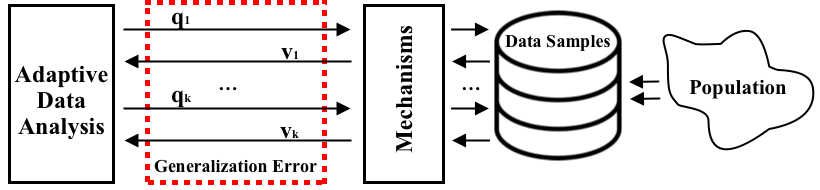
\includegraphics[width=0.7\columnwidth]{overview.png}
    \caption{Overview of our Adaptive Data Analysis model.
    We have a population that we are interested in studying, and a dataset containing individual samples from this population. 
    The adaptive data analysis we are interested in running has access to the dataset through queries of some pre-determined family (e.g., statistical or linear queries) mediated by a mechanism. 
    This mechanism uses randomization to reduce the generalization error of the queries issued to the data.}
    \label{fig:adaptivity-model-overview}
\vspace{-0.5cm}
\end{figure}

A line of work initiated by \cite{DworkFHPRR15}, \cite{HardtU14} posed the question: Can we design \emph{general-purpose} methods that ensure generalization in the presence of adaptivity, together with guarantees on their accuracy?  
The idea that has emerged in these works is to use randomization to help ensure generalization. 
Specifically, these works have proposed to mediate the access of an adaptive data analysis to the data by means of queries from some pre-determined family (we will consider here a specific family of queries often called "statistical" or "linear" queries) that are sent to a  \emph{mechanism} which uses some randomized process to guarantee that the result of the query does not depend too much on the specific
sampled dataset. 
This guarantees that the result of the queries generalizes well. This approach is described in Fig.~\ref{fig:adaptivity-model-overview}.  
This line of work has identified many new algorithmic techniques for ensuring generalization in adaptive data analysis, leading to algorithms with greater statistical power than all previous approaches. Common methods proposed by these works include, the addition of noise to the result of a query, data splitting, etc. Moreover, these works have also identified problematic strategies for adaptive analysis, showing limitations on the statistical power one can hope to achieve. Subsequent works have then further extended the methods and techniques in this approach and further extended the theoretical underpinning of this approach, e.g.~\cite{dwork2015reusable,dwork2015generalization,BassilyNSSSU16,UllmanSNSS18,FeldmanS17,jung2019new,SteinkeZ20,RogersRSSTW20}.

A key development in this line of work is that the best method for ensuring generalization in an adaptive data analysis depends to a large extent on the number of \emph{rounds of adaptivity}, the depth of the chain of queries. 
As an informal example, the program $x \leftarrow q_1(D);y \leftarrow q_2(D,x);z \leftarrow q_3(D,y)$ has three rounds of adaptivity, since $q_2$  depends on $D$ not only directly because it is one of its input but also via the result of $q_1$, which is also run on $D$, and similarly,  $q_3$ depends on $D$ directly but also via the result of $q_2$, which in turn depends on the result of $q_1$.
The works we discussed above showed that, not only does the analysis of the generalization error depend on the number of rounds, but knowing the number of rounds actually allows one to choose methods that lead to the smallest possible generalization error - we will discuss this further in Section~\ref{sec:overview}. 

For example, these works showed that when an adaptive data analysis uses a large number of rounds of adaptivity then a low generalization error can be achieved by a mechanism  
adding to the result of each query Gaussian noise scaled to the number of rounds. When instead  an adaptive data analysis uses a small number of rounds of adaptivity then a low generalization error can be achieved by using more specialized methods, such as data splitting mechanism or the reusable holdout technique from~\cite{DworkFHPRR15}.
To better understand this idea, we show in Fig.~\ref{fig:generalization_errors} three experiments showcasing these situations.
More precisely, in Fig.~\ref{fig:generalization_errors}(a) we show the results of a specific analysis\footnote{We will use formally a program implementing this analysis (Fig.~\ref{fig:overview-example}) as a running example in the rest of the paper.} with two rounds of adaptivity.
This analysis can be seen as a classifier which first runs 400 non-adaptive queries on the first 400 attributes of the data, looking for correlations between the attributes and a label, and then runs one last query which depends on all these correlations.
Without any mechanism the generalization error of the last query is pretty large, and the lower generalization error is achieved when the data-splitting method is used.
Fig.~\ref{fig:generalization_errors}(c) shows how this situation also change with the number of queries. Specifically, it shows the root mean square error of the last \emph{adaptive} query when the numbers queries varies. This also highlight the fact that different mechanisms, for the same analysis, produce results with very different generalization error.
In Fig.~\ref{fig:generalization_errors}(b), we show the results of a specific analysis\footnote{We will present this analysis formally in Section~\ref{sec:examples}.} with four hundreds rounds of adaptivity.
At each step, this analysis runs an adaptive query based on the results of the previous ones. Without any mechanism, the generalization error of most of the queries is pretty large, and this error can be lowered by using Gaussian noise. 
{\small
\begin{figure}
\centering
\begin{subfigure}{.32\textwidth}
\begin{centering}
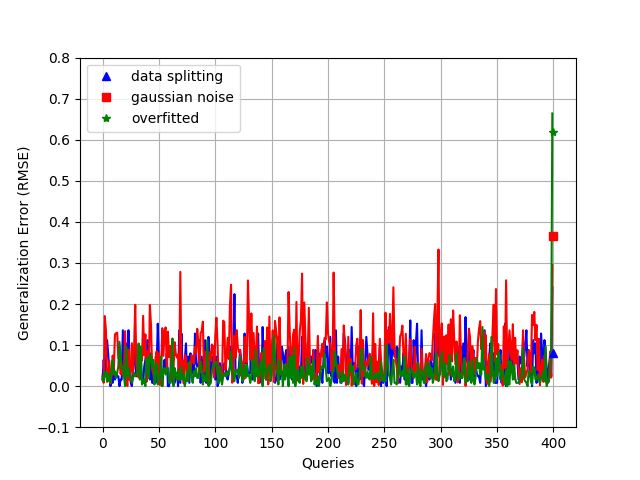
\includegraphics[width=1.0\textwidth]{tworound.png}
\caption{}
\end{centering}
\end{subfigure}
\quad
\begin{subfigure}{.32\textwidth}
\begin{centering}
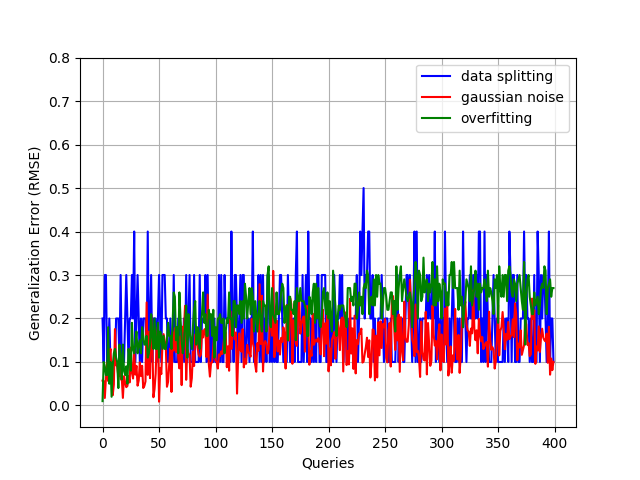
\includegraphics[width=1.0\textwidth]{multipleround.png}
\caption{}
\end{centering}
\end{subfigure}
\begin{subfigure}{.32\textwidth}
\begin{centering}
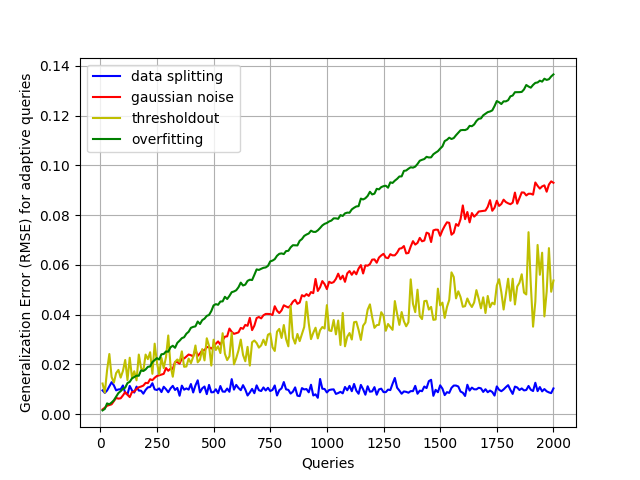
\includegraphics[width=1.0\textwidth]{twoRounds-rmse-fourmechs.png}
\caption{}
\end{centering}
\end{subfigure}
\vspace{-0.5cm}
 \caption{
 The generalization errors of two adaptive data analysis examples, under different choices of mechanisms.
 (a) Data analysis with 2 rounds adaptivity, 
 (b) Data analysis with 400 rounds adaptivity.
 (c) Same Data analysis as (a) with different query numbers.
}
\label{fig:generalization_errors}
\vspace{-0.6cm}
\end{figure}
}
%gap

This scenario motivates us to explore the design of program analysis techniques that can be used to estimate the number of \emph{rounds of adaptivity} that a program implementing a data analysis can perform. These techniques could be used to help a data analyst in the choice of the mechanism to use,
and they
could ultimately be integrated into a tool for adaptive data analysis such as the \emph{Guess and Check} framework by~\cite{RogersRSSTW20}. 

The first problem we face is \emph{how to formally define} a model for adaptive data analysis which is general enough to support the methods we discussed above and which would permit to formulate the notion of adaptivity these methods use. We take the approach of designing a programming framework for submitting queries to some \emph{mechanism} giving access to the data mediated by one of the techniques we mentioned before, e.g., adding Gaussian noise, randomly selecting a subset of the data, using the reusable holdout technique, etc. In this approach, a program models an \emph{analyst} asking a sequence of queries to the mechanism. The mechanism runs the queries on the data applying one of the methods above and returns the result to the program. The program can then use this result to decide which query to run next. Overall, we are interested in controlling the generalization of the query results returned by the mechanism, by means of the adaptivity. 

The second problem we face is \emph{how to define the adaptivity of a given program}.
Intuitively, a query $Q$ may depend on another query $P$, if there are two values that $P$ can return which affect in different ways the execution of $Q$. 
For example, as shown in \cite{dwork2015reusable}, and as we did in our example in Fig.~\ref{fig:generalization_errors}(a), one can design a machine learning algorithm for constructing a classifier which first computes each feature's correlation with the label via a sequence of queries, and then constructs the classifier based on the correlation values. If one feature's correlation changes, the classifier depending on features is also affected.  
This notion of dependency builds on the execution trace as a \emph{causal history}. In particular, we are interested in the history or provenance of a query up until this is executed, we are not then concerned about how the result is used --- except for tracking whether the result of the query may further cause some other query. This is because we focus on the generalization error of queries and not their post-processing. % 
To formalize this intuition as a quantitative program property,
we use a trace semantics recording the execution history of programs on some given input --- and we create a dependency graph, where the dependency between different variables (queries are also assigned to variables) is explicit and track which variable is associated with a query request. We then enrich this graph with weights describing the number of times each variable is evaluated in a program evaluation starting with an initial state. The adaptivity is then defined as the length of the walk visiting most query-related variables on this graph\footnote{Formally, graphs will be well-defined only for terminating programs, this will guarantee that the longest walk is finite}. In other words, we define adaptivity as a \emph{quantitative form of program dependency}.

% \jl{ 
% To define adaptivity in our programming framework, we consider a weighted dependency graph over variables assigned in the program, where each edge is built by a semantics dependency relation between these variables. The dependency relation relies on the trace semantics of our programming framework which records the execution history of programs implementing adaptive data analysis. 
% %The novelty comes from the definition of relation of dependency between nodes, which consists of the edge in the graph. For now, we can think of each node is associated with a variable, storing the value assigned to its variable 
% }
% \jl{The general idea beneath this dependency relation is that modifying the value of some variable in an execution trace will later affect the following execution trace.
% By tracking if a variable is assigned by a query or not, we are able to distinguish whether one query may depend on the other.}

The third problem we face is \emph{how to estimate the adaptivity of a given program}. 
The adaptive data analysis model we consider and our definition of adaptivity suggest that for this task we can use a  program analysis that is based on some form of dependency analysis. This analysis needs to take into consideration:
1) the fact that, in general, a query $Q$ is not a monolithic block but rather it may depend, through the use of variables and values, on other parts of the program. Hence, it needs to consider some form of data flow analysis. 
2) the fact that, in general, the decision on whether to run a query or not may depend on some other value. Hence, 
 it needs to consider some form of control flow analysis.
 3) the fact that, in general, we are not only interested in whether there is a dependency or not, but in the length of the chain of dependencies. Hence, it needs to consider some quantitative information about the program dependencies. 
 
To address these considerations and be able to estimate a sound upper bound on the adaptivity of a program, 
we develop a static program analysis algorithm, named {\THESYSTEM}, which combines data flow and control flow analysis with reachability bound analysis~\cite{GulwaniZ10}. This combination gives tighter bounds on the adaptivity of a program than the ones one would achieve by directly using the data and control flow analyses or the ones that one would achieve by directly using reachability bound analysis techniques alone. We evaluate {\THESYSTEM} on a number of examples showing that it is able to efficiently estimate precise upper bounds on the adaptivity of different programs. 
All the proofs and extended definitions can be found in the supplementary material.

To summarize, our work aims at the design of a static analysis for programs implementing adaptive analysis that can estimate their rounds of adaptivity. Specifically, our contributions are:
\begin{enumerate}
    \item A programming framework for adaptive data analyses where programs represent analysts that can query generalization-preserving mechanisms mediating the access to some data. 
    \item 
    A formal definition of the notion of adaptivity under the analyst-mechanism model. 
    This definition is built on a variable-based dependency graph that is constructed using sets of program execution traces.
    \item 
    A static program analysis algorithm {\THESYSTEM} combining data flow, control flow and  reachability bound analysis in order to provide tight bounds on the adaptivity of a program.
    \item A soundness proof of the program analysis showing that the adaptivity estimated by {\THESYSTEM} bounds the true adaptivity of the program. 
    \item An implementation of {\THESYSTEM} and an experimental evaluation of the bounds this implementation provides on several examples.
\end{enumerate}

\section{Overview}
\label{sec:overview}
\subsection{Some results in Adaptive Data Analysis}
%\wq{I think we can move this subsection into appendix. Maybe just leave theorm 1.2 and 1.3}
%\jl{I don't agree}
In Adaptive Data Analysis an \emph{analyst} is interested in studying some distribution $\dist$ over some domain $\univ$.  Following previous works~\cite{DworkFHPRR15,HardtU14,BassilyNSSSU16}, we focus on the setting where the analyst is interested in answers to \emph{statistical queries} (also known as \emph{linear queries}) over the distribution.  A statistical query is usually defined by some function $\qquery \from \univ \to [-1,1]$ (often other codomains such as $[0,1]$ or $[-R,+R]$, for some $R$, are considered).  The analyst wants to learn the \emph{population mean}, which is defined as 
$\qquery(\dist) = \ex{\sample \sim \dist}{\qquery(\sample)}$. 
%
We assume that the distribution $\dist$ can only be accessed via a set of \emph{samples} $\sample_1,\dots,\sample_n$ drawn independently and identically distributed (i.i.d.) from $\dist$.  These samples are held by a mechanism $\mech(\sample_1,\dots,\sample_n)$ who receives the query $\query$ and computes an answer 
$\answer \approx \qquery(\dist)$.
%
The na\"ive way to approximate the population mean is to use the \emph{empirical mean}, which (abusing notation) is defined as 
$\qquery(\sample_1,\dots,\sample_n) = \frac{1}{n} \sum_{i=1}^{n} \qquery(X_i)$.
However, the mechanism $M$ can adopt some methods for improving the generalization error $| a- \qquery(\dist)|$.

In this work we consider analysts that ask a sequence of $k$ queries $\qquery_1,\dots,\qquery_k$.  If the queries are all chosen in advance, independently of the answers \highlight{$a_1,\dots,a_k$} of each other, then we say they are \emph{non-adaptive}.  If the choice of each query $\qquery_j$ depends on the prefix $\qquery_1,\answer_1,\dots,\qquery_{j-1},\answer_{j-1}$ then they are \emph{fully adaptive}.  An important intermediate notion is \emph{$\qrounds$-round adaptive}, where the sequence can be partitioned into $\qrounds$ batches of non-adaptive queries.  Note that non-adaptive queries are $1$-round and fully adaptive queries are $k$-round adaptive.

We now review what is known about the problem of answering $r$-round adaptive queries.  
\begin{thm}[\cite{BassilyNSSSU16}] 
\label{thm:nonadapt-adapt}
\begin{enumerate}

\item For any distribution $\dist$, and any $k$ \emph{non-adaptive} statistical queries, \highlight{with high probablity,} 
% $$
$
\max_{j=1,\dots,k} | \answer_j - \qquery_j(\dist) | = O\left( \sqrt{\frac{\log k}{n}}  \right)
% $$
$.
%
\item For any distribution $\dist$, and  any $k$  \emph{$\qrounds$-round adaptive} statistical queries, with $\qrounds \geq 2$, \highlight{with high probablity,} the empirical mean (rounded to an appropriate number of bits of precision)\footnote{With infinite precision even two queries may give unbounded error, when the first query's result encodes the whole data.} satisfies:\\
% $$
$
\max_{j=1,\dots,k} | \answer_j - \qquery_j(\dist) | = O\left( \sqrt{\frac{k}{n}}  \right)
% $$
$
\end{enumerate}
\end{thm}
In fact, these bounds are tight (up to constant factors) which means that even allowing one extra round of adaptivity leads to an exponential increase in the generalization error, from $\log k$ to $k$.

\citet{DworkFHPRR15} and \citet{BassilyNSSSU16} showed that by using carefully calibrated Gaussian noise in order to limit the dependency of a single query on the specific data instance, one 
can actually achieve much stronger generalization error as a function of the number of queries, specifically.
\begin{thm}[\cite{DworkFHPRR15, BassilyNSSSU16}] \label{thm:gaussiannoise} For any distribution $\dist$, any $k$, any $\qrounds \geq 2$ and any \emph{$\qrounds$-round adaptive} statistical queries, if we answer queries with carefully calibrated Gaussian noise, \highlight{with high probablity,}  we have:
\begin{center}
  $
\max_{j=1,\dots,k} | \answer_j - \qquery_j(\dist) | = O\left( \frac{\sqrt[4]{k}}{\sqrt{n}}  \right)
$  
\end{center}
\end{thm}
% Notice that in order to Theorem~\ref{thm:gaussiannoise} has different quantification in that the optimal choice of mechanism depends on the number of queries.  Thus, we need to know the number of queries \emph{a priori} to choose the best mechanism.
More interestingly, \citet{DworkFHPRR15}
also gave a refined bounds that can be achieved with different mechanisms depending on the number of rounds of adaptivity.   \begin{thm}[\cite{DworkFHPRR15}] \label{thm:gaussiannoise2} For any $r$ and $k$, there exists a mechanism such that for any distribution $\dist$, and any $\qrounds \geq 2$ any \emph{$\qrounds$-round adaptive} statistical queries, \highlight{with high probablity,} it satisfies
\begin{center}
  $
\max_{j=1,\dots,k} | \answer_j - \qquery_j(\dist) | = O\left( \frac{r \sqrt{\log k}}{\sqrt{n}}  \right)
$  
\end{center}
\end{thm}
Notice that Theorem~\ref{thm:gaussiannoise2} has different quantification in that the optimal choice of mechanism depends on the number of queries {and number of rounds of adaptivity}.  This suggests that if one knows a good \emph{a priori upper bound on the number of rounds of adaptivity}, one can choose the appropriate mechanism and get a much better guarantee in terms of the generalization error.
As an example, as we can see in Fig.~\ref{fig:generalization_errors}, if we know that an algorithm is 2-rounds adaptive, we can choose data splitting as {the} mechanism, while if we know that an algorithm has many rounds of adaptivity we can choose Gaussian noise. It is worth to stress that by knowing the number of rounds of adaptivity one can also compute a concrete upper bound on the generalization error of a data analysis. This information allows one to have a quantitative, a priori, estimation of the effectiveness of a data analysis. 
This motivates us to design a static program analysis aimed at giving good \emph{a priori} upper bounds on the number of rounds of adaptivity of a program. 

{\small
\begin{figure}
\centering
\begin{subfigure}{.2\textwidth}
\begin{centering}
$
    \begin{array}{l}
    \kw{towRounds(k)} \triangleq \\
           \clabel{ \assign{a}{0}}^{0} ;
            \clabel{\assign{j}{k} }^{1} ; \\
            \ewhile ~ \clabel{j > 0}^{2} ~ \edo ~ \\
            \Big(
             \clabel{\assign{x}{\query(\chi[j] \cdot \chi[k])} }^{3}  ; \\
             \clabel{\assign{j}{j-1}}^{4} ;\\
            \clabel{\assign{a}{x + a}}^{5}       \Big);\\
            \clabel{\assign{l}{\query(\chi[k]*a)} }^{6}\\
        \end{array}
$
\caption{}
\end{centering}
\end{subfigure}
\begin{subfigure}{.4\textwidth}
%}
\qquad
\begin{centering}
\begin{tikzpicture}[scale=\textwidth/16cm,samples=250]
\draw[] (0, 10) circle (0pt) node
{{ $a^0: {}^{\lambda \trace_0. 1}_{0}$}};
\draw[] (0, 7) circle (0pt) node
{\textbf{$x^3: {}^{\lambda \trace_0. \env(\trace_0) k}_{1}$}};
\draw[] (0, 4) circle (0pt) node {{ $a^5: {}^{\lambda \trace_0. \env(\trace_0) k}_{0}$}};
\draw[] (0, 1) circle (0pt) node
{{ $l^6: {}^{\lambda \trace_0. 1}_{1}$}};
% Counter Variables
\draw[] (8, 9) circle (0pt) node {\textbf{$j^1: {}^{\lambda \trace_0. 1}_{0}$}};
\draw[] (8, 6) circle (0pt) node {{ $j^4: {}^{\lambda \trace_0. \env(\trace_0) k}_{0}$}};
%
% Value Dependency Edges:
\draw[ ultra thick, -latex, densely dotted,] (0, 1.5)  -- (0, 3.5) ;
\draw[ ultra thick, -latex, densely dotted,] (0, 4.5)  -- (0, 6.5) ;
\draw[ thick, -latex] (0, 4.5)  to  [out=-230,in=230]  (0, 9.5) ;
\draw[ thick, -Straight Barb] (1.5, 3.8) arc (120:-200:1);
\draw[ thick, -Straight Barb] (9, 6.5) arc (150:-150:1);
\draw[ thick, -latex] (8, 6.5)  -- (8, 8.5) ;
\draw[ thick, -latex] (0, 1.5)  to  [out=-230,in=230]  (0, 9.5) ;
% Control Dependency
\draw[ thick,-latex] (2, 7)  -- (6, 9) ;
\draw[ thick,-latex] (2, 4.5)  -- (6, 9) ;
\draw[ thick,-latex] (2, 7)  -- (6, 6) ;
\draw[ thick,-latex] (2, 4.5)  -- (6, 6) ;
\end{tikzpicture}
\caption{}
\end{centering}
\end{subfigure}
   \begin{subfigure}{.36\textwidth}
   \begin{centering}
   \begin{tikzpicture}[scale=\textwidth/18cm,samples=200]
\draw[] (0, 10) circle (0pt) node
{{ $a^0: {}^1_{0}$}};
\draw[] (0, 7) circle (0pt) node
{\textbf{$x^3: {}^{k}_{1}$}};
\draw[] (0, 4) circle (0pt) node
{{ $a^5: {}^{k}_{0}$}};
\draw[] (0, 1) circle (0pt) node
{{ $l^6: {}^{1}_{1}$}};
% Counter Variables
\draw[] (5, 9) circle (0pt) node {\textbf{$j^1: {}^{1}_{0}$}};
\draw[] (5, 6) circle (0pt) node {{ $j^4: {}^{k}_{0}$}};
%
% Value Dependency Edges:
\draw[ ultra thick, -latex, densely dotted,] (0, 1.5)  -- (0, 3.5) ;
\draw[ ultra thick, -latex, densely dotted,] (0, 4.5)  -- 
% node [left] {\highlight{$\trace_0 \to \env(\trace_0) k $}}
(0, 6.5) ;
\draw[ thick, -latex] (0, 4.5)  to  [out=-230,in=230]  
% node [left] {\highlight{$\trace_0 \to \env(\trace_0) k $}}
(0, 9.5) ;
\draw[ thick, -Straight Barb] (1.5, 3.5) arc (120:-200:1);
\draw[ thick, -Straight Barb] (6.5, 6.5) arc (150:-150:1);
    % The Weight for this edge
    % \draw[](9, 6) node [] {\highlight{$\trace_0 \to \env(\trace_0) k  $}};
\draw[ thick, -latex] (5, 6.5)  -- (5, 8.5) ;
% Control Dependency
\draw[ thick,-latex] (1.5, 7)  -- (4, 9) ;
\draw[ thick,-latex] (1.5, 4)  -- (4, 9) ;
\draw[ thick,-latex] (1.5, 7)  -- (4, 6) ;
\draw[ thick,-latex] (1.5, 4)  -- (4, 6) ;
\draw[ thick, -latex] (0, 1.5)  to  [out=-230,in=230]  (0, 9.5) ;
\end{tikzpicture}
\caption{}
   \end{centering}
   \end{subfigure}
\vspace{-0.4cm}
 \caption{(a) The program $\kw{towRounds(k)}$, an example 
%  of a program 
with two rounds of adaptivity (b) The corresponding execution-based dependency graph (c) The program-based dependency graph from $\THESYSTEM$.
}
\label{fig:overview-example}
% \vspace{-0.8cm}
\end{figure}
}


\subsection{ {\THESYSTEM} formally through an example.}
We illustrate the key technical components of our framework through a simple adaptive data analysis with two rounds of adaptivity.
% They are 1. the query while language for expressing a data analysis formally, 2. the definition of \emph{adaptivity} (\emph{adaptivity} is the short for \emph{rounds of adaptivity} used in the rest of the paper) based on the language semantics, and 3. the static analysis algorithm providing a sound upper bound on a data analysis' adaptivity.
% }
% \detailed{
% In "two rounds strategy" analysis, the analyst asks in total $k+1$ queries to the mechanism in two phases, the symbol $k$ is an input from the data analyst of this strategy and has no limit on the kind, which can be a constant, or a symbol or even an expression such as $(k+3)*2$.
% } 
%
In this analysis, an analyst asks $k+1$ queries to a mechanism in two phases.
In the first phase, the analyst asks $k$ queries and stores the answers that are provided by the mechanism. In the second phase, the analyst constructs a new query based on the results of the previous $k$ queries and sends this query to the mechanism. 
The mechanism is abstract here and our goal is to use static analysis to provide an upper bound on adaptivity to help choose the mechanism.
This data analysis assumes that the data domain $\univ$ 
contains at least $k$ numeric attributes 
(every query in the first phase focuses on one), which we index just by natural numbers.
The implementation of this data analysis in the language of {\THESYSTEM} is presented in Fig.~\ref{fig:overview-example}(a).

The {\THESYSTEM} language extends a standard while language\footnote{Programs components are labeled, so that we can uniquely identify every component.} with a query request constructor denoted $\query$.
 Queries have the form $\query(\qexpr)$, where $\qexpr$ is a special expression (see syntax in Section~\ref{sec:loop_language}) 
representing a function $\from \univ \to U$ on rows \highlight{of the hidden database the corresponding query will ask}.
We use $U$ to denote the codomain of queries and it could be $[-1,1]$, $[0,1]$ or $[-R,+R]$, for some $R$ we consider. This function characterizes the linear query we are interested in running. Indeed, as we discussed in the previous section, linear queries compute the empirical mean of a function on rows 
--- we use $\chi$ to abstract a possible row in the database \highlight{which distinguishes $\univ$ for a domain of a row}.
 As an example, $x \leftarrow \query(\chi[j] \cdot \chi[k])$ computes an approximation, according to the used mechanism, of the empirical mean of the product of the $j^{th}$ attribute and $k^{th}$ attribute, identified by $\chi[j] \cdot \chi[k]$. Notice that we don't materialize the mechanism but we assume that it is implicitly run when we execute the query. 
 In Fig.~\ref{fig:overview-example}(a), the queries inside the while loop correspond to the first phase of the data analysis and compute \highlight{the sum of the empirical mean of
the product of the $j$th attribute with the $k$th attribute}. 
The query outside the loop corresponds to the second phase and computes an approximation of the empirical mean where each record is weighted by the sum of the empirical mean of the first $k$ attributes.


This example is intuitively 2-rounds adaptive since we have two clearly distinguished phases, and the queries that we ask in the first phase do not depend on each other (the query $\chi[j] \cdot \chi[k]$ at line $3$ only relies on the counter $j$ and input $k$), while the last query 
(at line 6) depends on the results of all the previous queries. 
However, capturing this concept formally is surprisingly difficult. The difficulty comes from the fact that a query can depend on the result of another query in multiple ways, by means of data dependency or control dependency.
% \mg{this is weaker than it was in the previous submission.}

%%%%%%%%%%%%%%%%%%%%%%%%%%%%%%%%%%%Some details that might be useful when make passes %%%%%%%%%%%%%%%%%
% \jl{ The $\bullet$ stands for no query, for instance, the second event in the trace $(j, 1, \env(\trace)k , \bullet) $ tells us the assignment at line $1$ does not request a query.} \jl{The third event is a testing event corresponding to the guard of the while loop at line $2$. The evaluation of the query request in the second phase is tracked in }
% % \jl{ 
% The $\bullet$ is a default value for non-query event, 
% for instance, the second event in the trace $(j, 1, K , \bullet) $ tells us the assignment at line $1$ does not request a query.
% The third event is a testing event corresponding to the guard of the while loop at line $2$. The evaluation of the query request in the second phase is tracked in 
% % }
\subsubsection{Adaptivity definition}
\label{sec:adaptivity-informal}
%%%%%%%%%%%%%%%%%%%%%%%%%%%%%%%%%%% Details Below that might be useful when make passes %%%%%%%%%%%%%%%%%
% \detailed{To formally define the adaptivity, we build a directed graph representing the possible dependencies between queries of a program and we call this graph: execution-based dependency graph. The vertices represent the assigned program variables and the edges satisfy the dependency relations between vertices.   Fig.~\ref{fig:overview-example}(b) is the execution dependency graph we build based on the "two rounds strategy program" in Fig.~\ref{fig:overview-example}(a). In brief, the graph is built by collecting the assigned variables with labels of the target program as vertices, which are $a^0$, $j^1$,...$a^5$,$l^6$. We check if there is an edge between two vertices by our dependency relation over two labeled variables (defined in Section~\ref{sec:dep_adaptivity} ). This dependency relation relies on the execution of the program recorded by a trace generated by our trace semantics, which is the reason we call this graph "execution-based". 
% Intuitively from Fig.~\ref{fig:overview-example}(a), the query in the second phase (at line 6) depends on the query results in the first phase stored in $a$ at line 5, and the variable $a$ also relies on the queries at line 3. Correspondingly, we have two edges $(l^6, a^5)$ and $(a^5, x^3)$ in our execution-based dependency graph in Fig.~\ref{fig:overview-example}(b). Besides, we also have special edge which is a circle, to track any variable being updated with its previous value recursively. For instance, the counter $j$ and the variable $a$ are updated based on previous values $k$ times in the first phase and we see two circle edges on $a^5$ and $j^4$.}

The central property we are after in this work is the \emph{adaptivity of a program}. We define formally this notion in three steps, which we will describe in details in Section~\ref{sec:adaptivity}. First, we define a notion of dependency, or better \emph{may-dependency}, between variables. To do this we take inspiration from previous works on dependency analysis and information flow control and we say that a variable \emph{may depend} on another one if changing the execution of the latter can affect the execution of the former. 
We can see in Fig.~\ref{fig:overview-example}(a) that the value of the variable $l$, which corresponds to the result of the execution of the query in the second phase (in the command with label 6), is affected by the value of the variable $x$, which corresponds to the result of the execution of the query at line 3 in the first phase, via the variable $a$.
To formally define this notion of dependency, as in information flow control, we use the execution history of programs recorded by a trace semantics (see Definition~\ref{def:var_dep}).
% \mg{Please, double check that I refer to the right definition. }  

Second, we build an annotated weighted directed graph representing the possible dependencies between labeled variables. We call this graph \emph{semantics-based dependency graph} to stress that this graph summarizes the dependencies we could see if we knew the overall behavior of the program. 
The vertices of the graph are the assigned program variables with the label of their assignments, edges are pairs of labeled variables which satisfy the dependency relations, weights are functions associated with vertices and describe the number of times the assignment corresponding to the vertex is executed when the program is run in a given starting state\footnote{In our trace semantics the state is recorded in the trace, so an initial state is actually represented by an initial trace. We will use this terminology in later sections.}, and the annotations, which we call \emph{query annotations}, are bits associated with vertices and describe if the corresponding assignment comes from a query (1) or not (0).
The \emph{semantics-based dependency graph} of the $\kw{twoRounds(k)}$ program
we gave in Fig.~\ref{fig:overview-example}(a) is described in Fig.~\ref{fig:overview-example}(b) (we use dashed arrows for two edges that will be highlighted in the next step, for the moment these can be considered similar to the other edges---i.e. solid arrows). We have all the variables that are assigned in the program with their labels, and edges representing dependency relations between them. 
For example, we have two edges $(l^6, a^5)$ and $(a^5, x^3)$ describing the dependency between the variables assigned by queries. The vertices $l^6$ and $x^3$ are the only ones with query annotation $1$ (the subscript), since they are the only two variables that are in assignments involving  queries. Notice that the graph contains cycles---in this example it contains two self-loops. These cycles capture the fact that the variables $a^5$ and $j^4$ are updated at every iteration of the loop using their previous values. Cycles are essential to capture mutual dependencies like the ones that are generated in loops. Adaptivity is a quantitative notion, so capturing this form of dependencies is not enough. This is why we also use weights. The weight of a vertex is a function that given an initial state returns a natural number representing 
the number of times the assignment corresponding to a vertex is visited during the program execution starting in this initial state.  
For example, the vertex $l^{6}$ has weight {$\lambda \trace.1$} since for every initial state {$\trace$} the corresponding assignment will be executed one time, the vertex $a^5$ on the other hand has weight {$\lambda \trace. \env(\trace) k$ since the corresponding assignment will be executed a number of times that correspond to the value of $k$ in the initial state $\trace$, and $\env$ is the operator reading value of $k$ from $\trace$.
}

% It is a function which takes an initial state, $\trace_0$ as input,
% then executes the program, and counts the evaluation times of the query request $\clabel{\assign{l}{\query(\chi[k]*a)} }^{6}$ during the execution.
% % returns $1$ for every starting state, since 
% Since this query at line $6$ is outside of any loop, we are expecting this function always return the count $1$ given any initial state.
% The query annotation of this vertex is $1$, which  indicates that 
% $\clabel{\assign{l}{\query(\chi[k] * a)}}^6$ is a query request.
% For another vertex, $a^{5}:{}^{w_{a^{5}}}_0$ in the while loop, we expect its weight function
% returns different counts if the input initial traces have different initial value for $k$.
% Because $\clabel{\assign{a}{x + a}}^{5}$ will be executed different times if the input $k$  is different.
% Its subscript $0$ representing this is a non-query assignment.



% Besides, we also have special edge which is a circle, to track any variable being updated with its previous value recursively. 
% For instance, the loop counter $j$ and the variable $a$ are updated based on previous values $k$ times in the first phase and we see two circle edges on $a^5$ and $j^4$.

%%%%%%%%%%%%%%%%%%%%%%%%%%%%%%%%%%% Details Below that might be useful when make passes %%%%%%%%%%%%%%%%%
% \detailed{The existence of circle edge \jl{(there isn't a name 'circle edge', the terminology is cycle)}
%  allows our graph to express situation when a variable relies on its previous value recursively inside a while loop, but not show how many times of this reliance, which is necessary to define adaptivity. For instance, if we modify our two round example a little bit to make the query $query(\chi[j]\dot \chi[k])$ at line $3$ relies on its previous result to $query(\chi[j]\dot\chi[k] + x)$, then intuitively its adaptivity becomes $k+1$. To this end, we add quantitative information to our graph: weight on every vertex.
% The weight of a vertex is a function that given a starting state returns a natural number representing 
% the number of times the vertex is visited when the program is executed starting from this state.}
% \jl{The existence of cycle
%  allows our graph to handle the while loop.
% When the variable in a while loop relies on its value in the previous iterations, the cycle expresses this reliance.
% But it cannot express the times of this reliance.
% For instance, if we modify the command $3$
% of the $\kw{twoRounds(k)}$ example
% into $\clabel{\assign{x}{\query(\chi[j] \cdot \chi[k] + x)}}^3$. 
% Then $x$ in every iteration relies on the result in the previous iteration
% and the intuitive adaptivity becomes $k+1$. But we don't know the number $k$ by only constructing the edge $x^3 \to x^3$.
% To this end, we add quantitative information to our graph: weight on every vertex.
% The weight of a vertex is a function that given a starting state returns a natural number representing 
% the number of times the vertex is visited during the program execution.
% }
% Each vertex in this graph has a superscript representing its weight, and a subscript $1$ or $0$ telling if the vertex corresponds to a query or not. We will call this subscript a query annotation. 
% For example, in Fig.~\ref{fig:overview-example}(b), the vertex $l^{6}:{}^{w_1}_1$, 
% has weight $w_1$, a constant function which returns $1$ for every starting state, since 
% this query at line $6$ is at most executed once regardless of the initial trace.
% The query annotation of this vertex is $1$, which  indicates that 
% $\clabel{\assign{l}{\query(\chi[k] * a)}}^6$ is a query request.
% Another vertex, $x^{3}:{}^{w_k}_1$, appears in the while loop. 
% It has as weight a function $w_k$ that for every initial state returns the value that $k$ has in this state, since this is also the number the while loop will be iterated. 
% The node $j^{4}:{}^{w_k}_0$ has as a subscript $0$ representing a non-query assignment.
% \jl{
% For example, in Fig.~\ref{fig:overview-example}(b), the vertex $l^{6}:{}^{w_{l^{6}}}_1$, 
% has weight ${w_{l^{6}}}$. It is a function which takes an initial state, $\trace_0$ as input,
% then executes the program, and counts the evaluation times of the query request $\clabel{\assign{l}{\query(\chi[k]*a)} }^{6}$ during the execution.
% % returns $1$ for every starting state, since 
% Since this query at line $6$ is outside of any loop, we are expecting this function always return the count $1$ given any initial state.
% The query annotation of this vertex is $1$, which  indicates that 
% $\clabel{\assign{l}{\query(\chi[k] * a)}}^6$ is a query request.
% For another vertex, $a^{5}:{}^{w_{a^{5}}}_0$ in the while loop, we expect its weight function
% returns different counts if the input initial traces have different initial value for $k$.
% Because $\clabel{\assign{a}{x + a}}^{5}$ will be executed different times if the input $k$  is different.
% Its subscript $0$ representing this is a non-query assignment.
%
%It has as weight a function $w_k$ that for every initial state returns the value that $k$ has in this state, since this is also the number the while loop will be iterated. 
% The node $j^{4}:{}^{w_k}_0$ has as a subscript $0$ representing a non-query assignment.
% }
%%%%%%%%%%%%%%%%%%%%%%%%%%%%%%%%%%% Details Below that might be useful when make passes %%%%%%%%%%%%%%%%%
% \detailed{Since the edges between two vertices represent the fact that one program variable may depend on the other,
% we can define the program adaptivity with respect to a initial trace by means of a walk traversing the graph, visiting each vertex no more than its weight with respect to the initial trace, and visiting as many query nodes as possible.
% Still, look again at our example, we can see that
% in the walk along the dotted arrows,  $l^{6} \to a^5 \to x^3 $, there are $2$ vertices with query annotation $1$ and that this number is maximal, i.e. we cannot find another walk having more than $2$ vertices with query annotation $1$, under the assumption that $k \geq 1$. So the adaptivity of the program in Fig.~\ref{fig:overview-example}(a)  is $2$,
% as expected.
% }
Third, we can finally define adaptivity using the semantics-based dependency graph. We actually define this notion with respect to an initial state $\tau$, since different states can give very different adaptivities.  
We consider 
% the longest walk  that visits each vertex $v$ of the semantics-based dependency graph no more than the value that the weight $w_v$ assign to $\tau$, and visits as many query nodes as possible. 
\highlight{any} \remove{the} walk  that visits each vertex $v$ of the semantics-based dependency graph no more than the value that the weight $w_v$ applying to the initial state $\tau$, and visits the \highlight{maximal} number of query vertices.
The number of query vertices visited is the adaptivity of the program with respect to $\tau$.
Looking again at Fig.~\ref{fig:overview-example}(b), and assuming that $\tau(k) \geq 1$, we can see that the 
walk along the dashed arrows,  $l^{6} \to a^5 \to x^3 $ has two vertices with query annotation $1$, and we cannot find another walk having more than $2$ query vertices,\highlight{ ( $l^{6} \to x^3 $  with $2$ query vertices as well)}. So the adaptivity of the program in Fig.~\ref{fig:overview-example}(a) with respect to $\tau$ is $2$. If we consider an initial state $\tau$ such that $\tau(k)=0$ we have that the adaptivity with respect to $\tau$ is instead $1$. 
%%%%%%Gap: %%%%%%%%%%%%%%%%%%%%%%%%%%%%%%%%%%%%%%%%%%%%%%%%%%%%%%%%%%%%%%%%%%%%%%%%%%%%%%%%%%%%%%%%%%%%%%%%%%%%%%%%%%%%%%%%%%%%%%%%%%%%%%%%%%%%%%%
% \begin{figure}
%     \centering   
%     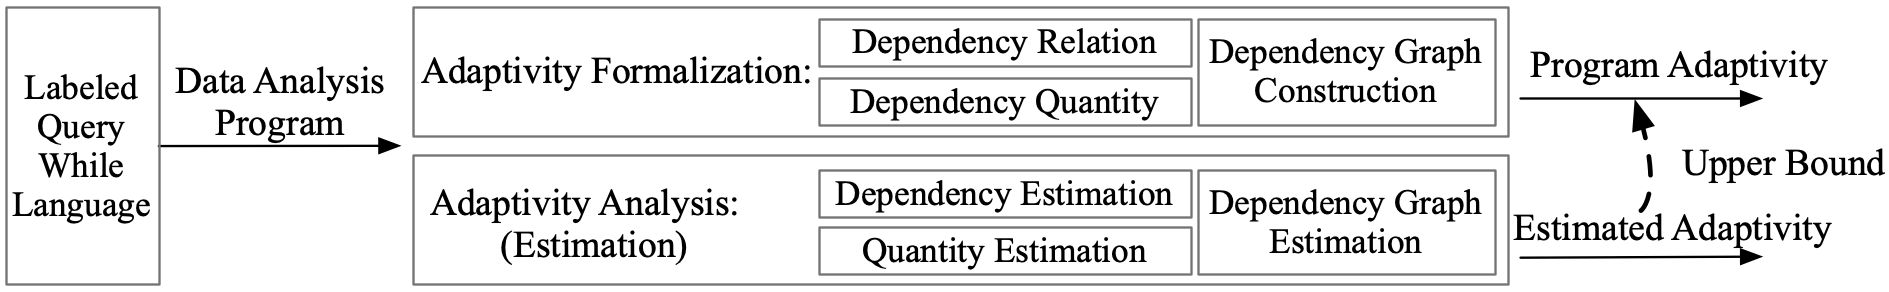
\includegraphics[width=1.0\textwidth]{architecture.png}
%     \vspace{-0.8cm}
%   \caption{High level architecture}
%     \label{fig:structure}
%     \vspace{-0.6cm}
% \end{figure}

\subsubsection{Static analysis}
%%%%%%%%%%%%%%%%%%%%%%%%%%%%%%% Previous Version Below that might be useful when make passes %%%%%%%%%%%%%%%%%
%  \detailed{The definition of adaptivity comes from the aforementioned execution-based dependency graph, 
%  our static analysis statically provides a sound upper bound on this adaptivity, via constructing another weighted graph, we call it estimated dependency graph. The upper bound is then found by searching a sound path with respect to our adaptivity in the generated graph. Different from the execution-based dependency which needs the trace from the execution, estimated one is built by our static analysis algorithm which takes the program itself as input. In brief, our algorithm is consist of a graph-generation algorithm, a weight computation algorithm and finally a path searching algorithm in the generated weighted graph.
%  }
%%%%%%%%%%%%%%%%%%%%%%%%%%%%%%% Previous Version Below that might be useful when make passes %%%%%%%%%%%%%%%%%
% \todo{In order to have a sound and accurate upper bound on the  adaptivity of a program $c$,
% we design a program analysis framework named {\THESYSTEM}.
% This framework composes two algorithms as shown in the double-stroke box and the dashed box in Fig.~\ref{fig:adaptfun}.
% The first algorithm in the double-stroke box combines the quantitative and dependency analysis techniques.
% It produces an estimated \emph{dependency graph} for a program.
% The second algorithm in the dashed box is a walk length estimation algorithm.
% It computes the upper bound on the program's \emph{adaptivity} over the estimated graph.}
% \jl{Since the definition of adaptivity comes from the aforementioned execution-based dependency graph, 
%  our static analysis statically provides a sound upper bound on this adaptivity via approximating this graph. The estimated graph is called \emph{estimated dependency graph}. 
%  The upper bound is then computed by searching the walk in this graph such that it can give a sound bound on the adaptivity.
%  Different from the execution-based dependency graph, the estimated one is produced by our static anlaysis algorithm, which only takes the program as input and does not rely on the execution history.
%  In brief, our algorithm is consist of a weighted graph-generation algorithm and a adaptivity computation algorithm over the graph.
%  }
 
 %%%%%%%%%%%%%%%%%%%%%%%%%%%%%%% Previous Version Above for Reference  %%%%%%%%%%%%%%%%%
To compute statically a sound and accurate upper bound on the \emph{adaptivity} of a program $c$,
we design a program analysis framework named {\THESYSTEM} which we will describe formally in Section \ref{sec:algorithm}. 
The structure of {\THESYSTEM} (Fig.~\ref{fig:adaptfun}) reflects in part the definition of adaptivity we discussed in the previous section. Specifically, {\THESYSTEM} is composed by two algorithms (the ones in dashed boxes in the figure), one for building a dependency graph, which we call \emph{estimated dependency graph}, and the other to estimate the adaptivity from this graph.  
The first algorithm generates the \emph{estimated dependency graph} using several program analysis techniques. Specifically,
 {\THESYSTEM} extracts the vertices and the query annotations by looking at the assigned variables of the program, it estimates the edges by using control flow and data flow analysis, and it estimates the weights by using symbolic reachability-bound analysis---weights in this graph are symbolic expressions over input variables. 
% This combined analysis allow us to obtain more accurate upper bounds than what we would obtain by using any of these single analysis technique in isolation.
The second algorithm estimates the
% longest 
walk which respects the weights and which visits the maximal number of query vertices.
%  as possible. 
The two algorithms together gives us an  upper bound on the program's \emph{adaptivity}.

 \begin{figure}
  \centering    
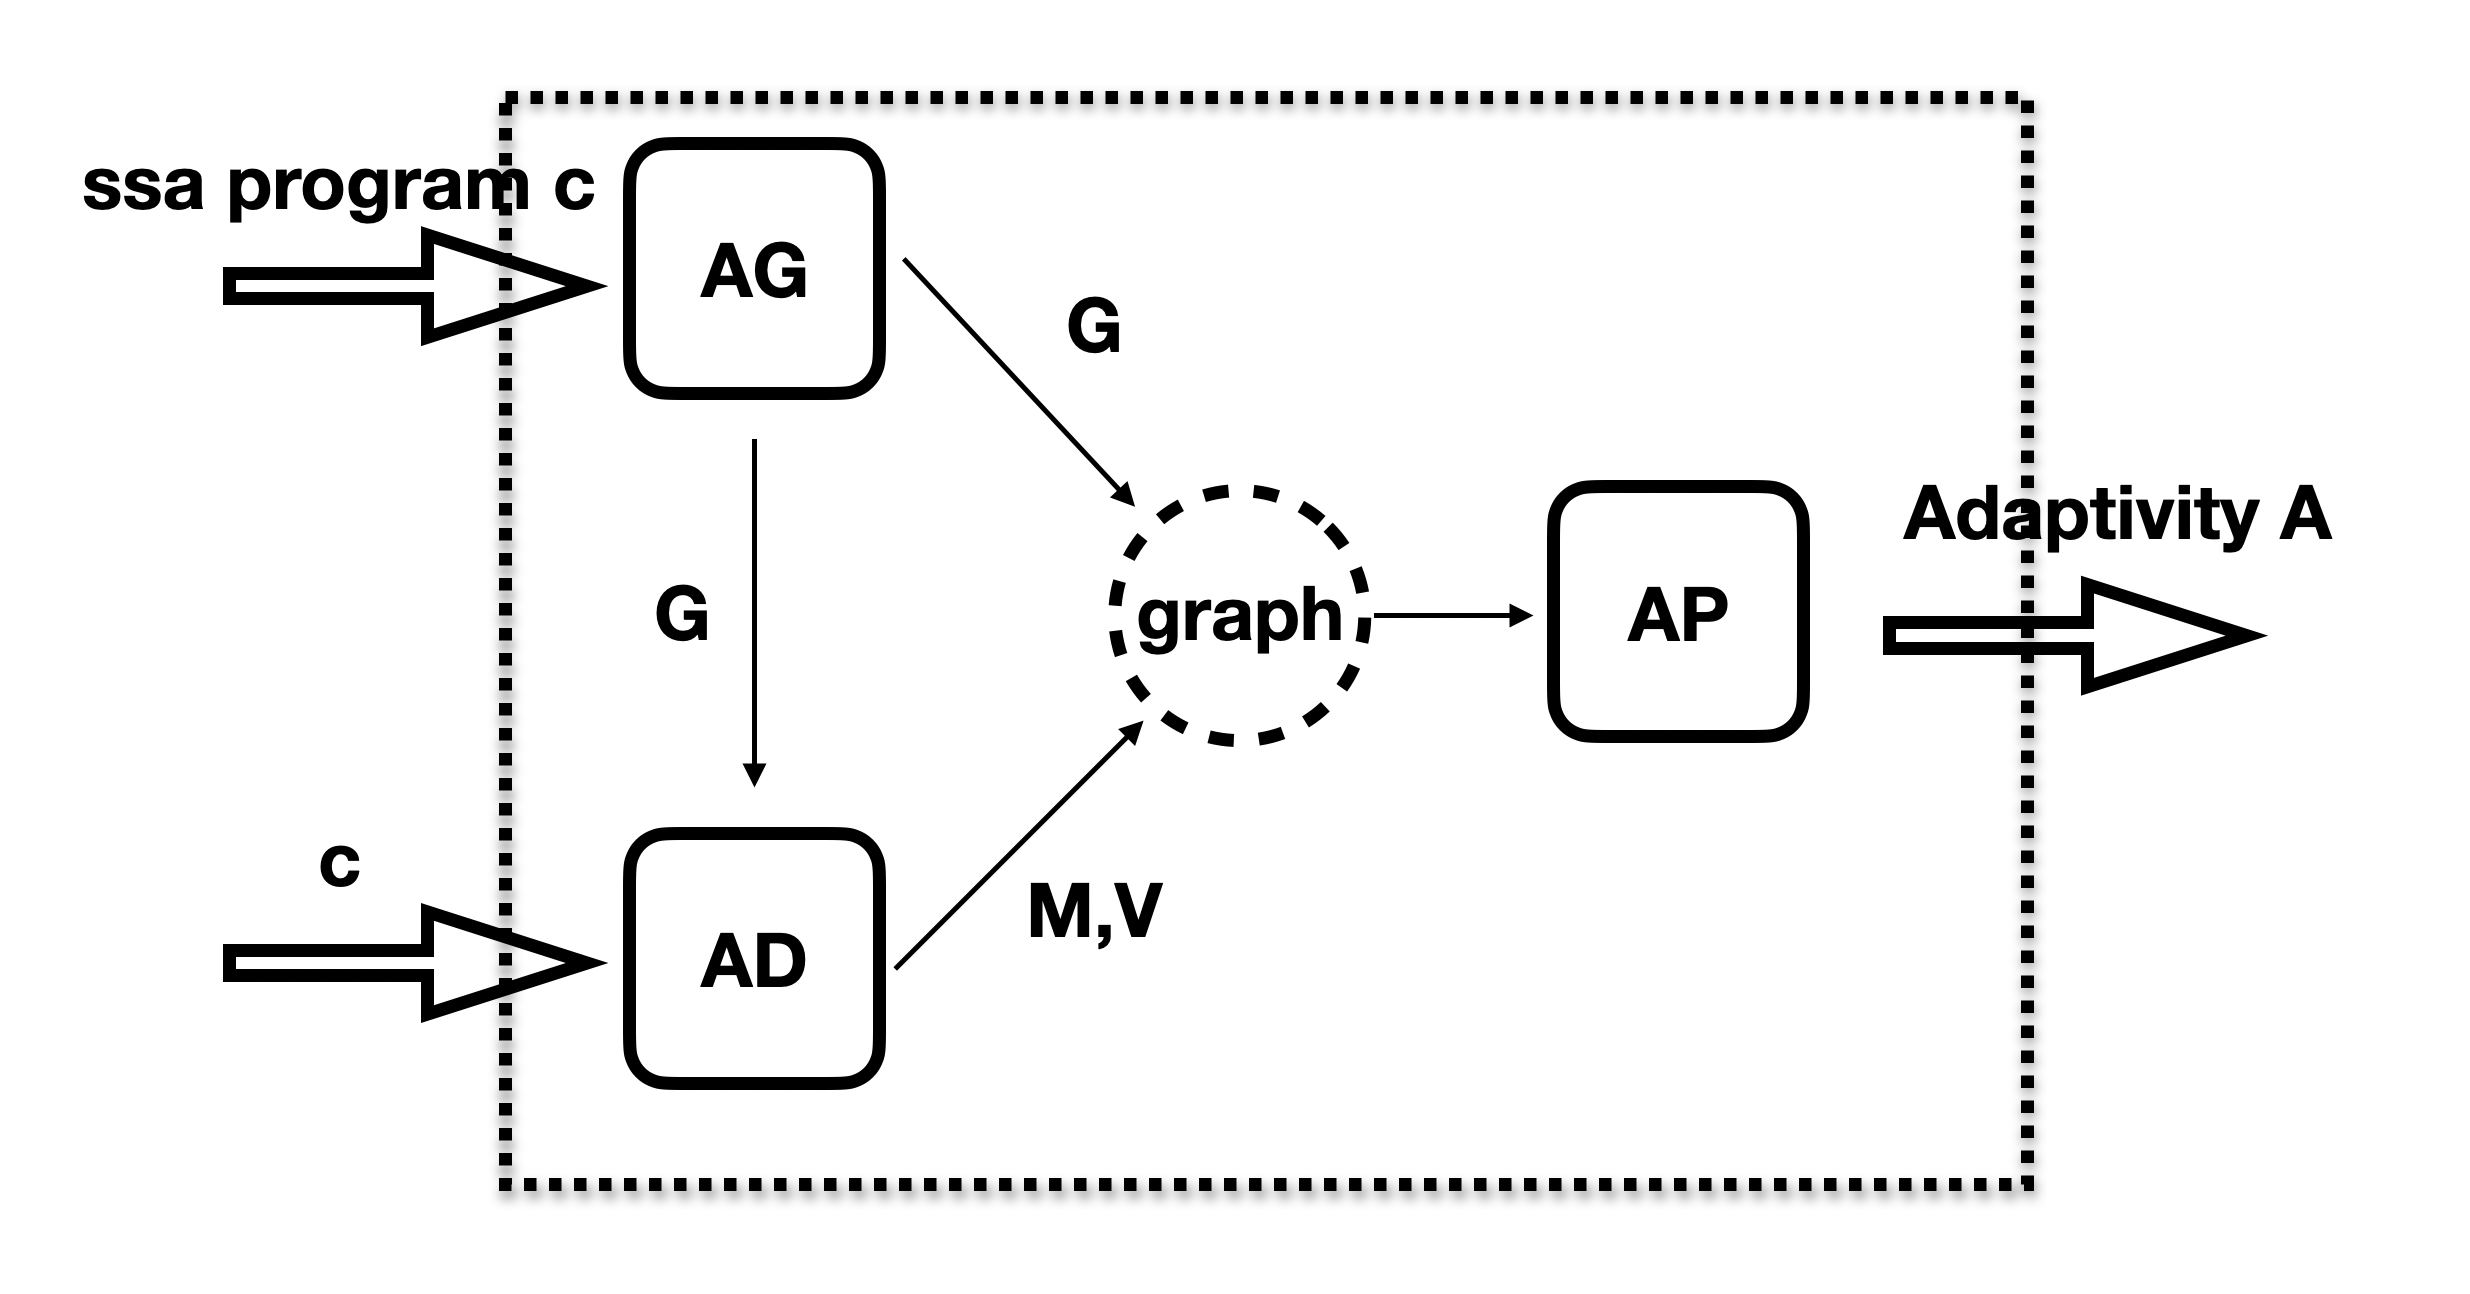
\includegraphics[width=1.0\columnwidth]{adapfun.png}
  \vspace{-0.8cm}
  \caption{The overview of {\THESYSTEM}}
  \label{fig:adaptfun}
  \vspace{-0.5cm}
\end{figure}

 
%%%%%%%%%%%%%%%%%%%%%%%%%%%%%%%%%%% Details Below that might be useful when others are making passes %%%%%%%%%%%%%%%%%
%   \detailed{Fig.~\ref{fig:overview-example}(c) is the resulting estimated graph of our static analysis algorithm which consumes the program in Fig.~\ref{fig:overview-example}(a).The edges are generated by our graph generation algorithm which combines control flow analysis and data flow analysis, presented in Section~\ref{sec:alg_edgegen}). We can easily see the generated graph in Fig.~\ref{fig:overview-example}(c) is a safe approximation of its execution-based counterpart in Fig.~\ref{fig:overview-example}(b), in the way that we can find a corresponding edge in Fig.~\ref{fig:overview-example}(c) for all the edges in Fig.~\ref{fig:overview-example}(b). We call the weight of every vertex computed by our algorithm as estimated weight,  }
%   estimated by using a reachability-bound estimation algorithm (presented in Section~\ref{sec:alg_weightgen}). \detailed{Different from the execution-based weight $w_1$ or $w_k$ in Fig.~\ref{fig:overview-example}(b) which is a function whose output relies on the initial trace, our estimated weight} can be symbolic and provide a sound upper bound on its execution-based weight of the corresponding vertex in the execution-based dependency graph. For instance, 
%   the estimated weight $k$ of the vertex $x^{3}$ in Fig.~\ref{fig:overview-example}(c) is a sound upper bound on the execution-based weight $w_k$ of vertex $x^{3}$ in Fig.~\ref{fig:overview-example}(b), with the same starting trace $\trace$, $w_k(\trace) \leq\trace(k)$. $\trace(k)$ means getting the value of variable $k$ in the trace $\trace$. The soundness of this step is proved in Theorem~\ref{thm:addweight_soundness}.   
%
We show in Fig.~\ref{fig:overview-example}(c) the estimated dependency graph that our static analysis algorithm returns for the program $\kw{twoRounds(k)}$ in Fig.~\ref{fig:overview-example}(a).
Vertices and query annotations are the same as the ones in Fig.~\ref{fig:overview-example}(b) and they are simply inferred by scanning the program.
As we said before, the edges are estimated using control flow and data flow analysis.
For the $\kw{twoRounds(k)}$ example, every edge in Fig.~\ref{fig:overview-example}(b) is precisely inferred by our combined analysis, this is why Fig.~\ref{fig:overview-example}(c) contains exactly the same edges.
The weight of every vertex is computed using a reachability-bound estimation algorithm which outputs a symbolic expression over the input variables, in the example only $k$, representing an upper bound on the number of times each assignment is executed.
% \wq{symbolic and provide a sound upper bound on its execution-based weight of the corresponding vertex in the execution-based dependency graph.
% $w_k(\trace) \leq \trace(k)$. $\trace(k)$ means getting the value of variable $k$ in the trace $\trace$. The soundness of this step is proved in Theorem~\ref{thm:addweight_soundness}.}
For example, consider the vertex $x^{3}$, its weight is $k$ and this provides an upper bound on the value returned by the weight function $\lambda \trace. \rho(\trace)k$ associated with vertex $x^{3}$ in Fig.~\ref{fig:overview-example}(b) for any initial state. 
% Indeed, 
% for any initial trace $\trace_0$, when $w_{x^{3}}(\trace_0)$ executes the program and counts the
% execution times of command $3$,
% we expect that this counts is at most the the loop iterations, i.e. $k$'s initial value from $\trace_0$.

The algorithm searching for the walk first finds a path $l^6:{}^1_1 \to a^5: {}^k_0 \to x^3: {}^k_1$, and then constructs a walk based on this path. Every vertex on this walk is visited once, and the number of vertices with query annotation $1$ in this walk is $2$, which is the upper bound we expect.
{It is worth noting here that $x^3$ and $a^5$ can only be visited once because there isn't an edge to go back to them, even though they both have the weight $k$}.
In this sense, instead of simply computing the weighted length of this path ($2k+1$) as adaptivity, the algorithm $\pathsearch$ computes the upper bound $2$. Note that $2$ is not always tight, for example when $k = 0$.
% \todo{Can you double check if this is clear?}
% \mg{I think we should add a sentence to say that this bound is actually not always tight.}


\section{Loop language }
\label{sec:loop_language}
%
%
\subsection{Labeled Language}
\[
\begin{array}{llll}
\mbox{Arithmetic Operators} 
& \oplus_a & ::= & + ~|~ - ~|~ \times 
%
~|~ \div \\  
\mbox{Boolean Operators} 
& \oplus_b & ::= & \lor ~|~ \land
\\
%
\mbox{Relational Operators} 
& \sim & ::= & < ~|~ \leq ~|~ == 
\\  
%
\mbox{Label} 
& l & := & \mathbb{N} 
\\ 
%
\mbox{Arithmetic Expression} 
& \aexpr & ::= & 
n ~|~ {x} ~|~ \aexpr \oplus_a \aexpr  
\\
%
\mbox{Boolean Expression} & \bexpr & ::= & 
%
\etrue ~|~ \efalse  ~|~ \neg \bexpr
 ~|~ \bexpr \oplus_b \bexpr
%
~|~ \aexpr \sim \aexpr 
\\
%
\mbox{Expression} & \expr & ::= & v ~|~ \aexpr \sep \bexpr ~|~ [\expr, \dots, \expr]
\\  
%
\mbox{Value} 
& v & ::= & { n \sep \etrue \sep \efalse ~|~ [] ~|~ [v, \dots, v]}  
\\
%
\mbox{Query Expression} 
& {\qexpr} & ::= 
& { \qval ~|~ \aexpr ~|~ \qexpr \oplus_a \qexpr ~|~ \chi[\aexpr]} 
\\
%
\mbox{Query Value} & \qval & ::= 
& {n ~|~ \chi[n] ~|~ \chi[n] \oplus_a  \chi[n] ~|~ n \oplus_a  \chi[n]
~|~ \chi[n] \oplus_a  n}
\\
%
\mbox{Labeled Command} 
& {c} & ::= &   [\assign {{x}}{ {\expr}}]^{l} ~|~  [\assign {{x} } {{\query(\qexpr)}}]^{l}
~|~ {\ewhile [ \bexpr ]^{l} \edo {c} }
\\
&&&
~|~ {c};{c}  
~|~ \eif([\bexpr]{}^l , {c}, {c}) 
~|~ [\eskip] 
\\
%
\mbox{Event} 
& \event & ::= & 
    ({x}, l, v) ~|~ ({x}, l, \qval, v)  ~~~~~~~~~~~ \mbox{Assignment Event} \\
&&& ~|~(\bexpr, l, v)   ~~~~~~~~~~~~~~~~~~~~~~~~~~~~~~~~~~ \mbox{Testing Event}
\\
%
% \mbox{Trace} & \trace
% & ::= & \cdot | \trace \cdot \event | \trace \tracecat \trace 
% \\
%
\mbox{Trace} & \trace
& ::= & [] ~|~ \event:: \trace ~|~ \trace \tracecat \trace  % \\
% %
% \mbox{Event Signature} & \sig
% & ::= & (x, l, n) | (x, l, n, \query) | (b, l, n)
% \\
% %
\end{array}
\]
% \todo{change trace notation into list, and update corresponding operator nations}
% \\
% \wqside{"$\cdot$" has two meanings? empty, delimit. Trace is list of event?}
We use following notations to represent the set of corresponding terms:
\[
\begin{array}{lll}
\mathcal{SVAR} & : & \mbox{Set of Variables}  
\\ 
%
\mathcal{VAL} & : & \mbox{Set of Values} 
\\ 
%
\mathcal{QVAL} & : & \mbox{Set of Query Values} 
\\ 
%
\cdom & : & \mbox{Set of Commands} 
\\ 
%
\eventset  & : & \mbox{Set of Events}  
\\
%
\eventset^{\asn}  & : & \mbox{Set of Assignment Events}  
\\
%
\eventset^{\test}  & : & \mbox{Set of Testing Events}  
\\
%
%%
\dbdom  & : & \mbox{{Set of Databases}} 
\\
%
{\mathcal{T}} & : & \mbox{Set of Traces}
\\
%
\qdom = {[-1,1]} & : & \mbox{{Domain of Query Results}}
\end{array}
\]
%
%
%
Environment $ \env : {\mathcal{T}}  \to \mathcal{SVAR} \to \mathcal{VAL} \cup \{\bot\}$
\[
\begin{array}{lll}
\env(\trace  \tracecat [(x, l, v)]) x \triangleq v
&
\env(\trace \tracecat [(x, l, \qval, v)]) x \triangleq v
&
\env(\trace \tracecat [(y, l, v)]) x \triangleq \env(\trace) x
\\
\env(\trace \tracecat [(b, l, v)]) x \triangleq \env(\trace) x
&
\env({[]} ) x \triangleq \bot
&
\end{array}
\]
%
%
% Query Environment $\qenv: \mathcal{T}  \to \mathcal{SVAR} \to \mathcal{QVAL} \cup \{\bot\}$
% \[
% \begin{array}{lll}
% \qenv(\trace \cdot (x, l, n, v) ) x \triangleq \qenv(\trace) x
% &
% \qenv(\trace \cdot (x, l, n, \qval, v) ) x \triangleq \qval
% &
% \qenv(\trace \cdot (y, l, n, v)) x \triangleq \env(\trace) x
% \\
% \qenv(\trace \cdot (b, l, n, v)) x \triangleq \env(\trace) x
% &
% \qenv(\cdot ) x \triangleq \bot
% &
% \end{array}
% \]
%

%
\subsection{Trace-based Operational Semantics for Language}
%
%
%
{
\begin{mathpar}
\boxed{ \config{\trace,\aexpr} \aarrow v \, : \, \mbox{Trace  $\times$ Arithmetic Expr $\Rightarrow$ Arithmetic Value} }
\\
\boxed{ \config{\trace, \bexpr} \barrow v \, : \, \mbox{Trace $\times$ Boolean Expr $\Rightarrow$ Boolean Value} }
\\
\boxed{ \config{\trace, \expr} \earrow v \, : \, \mbox{Trace $\times$ Expression $\Rightarrow$ Value} }
\\
\inferrule{ 
  \config{\trace, \aexpr} \aarrow v
}{
 \config{\trace,  \aexpr} 
 \earrow v
}
\and
\inferrule{ 
  \config{\trace, \bexpr} \barrow v
}{
 \config{\trace,  \bexpr} 
 \earrow v
}
\and
\inferrule{ 
  \config{\trace, \expr_1} \earrow v_1
  \cdots
  \config{\trace, \expr_n} \earrow v_n
}{
 \config{\trace,  [\expr_1, \cdots, \expr_n]} 
 \earrow [v_1, \cdots, v_n]
}
\and
\inferrule{ 
  \empty
}{
 \config{\trace,  v} 
 \earrow v
}
\\
\boxed{ \config{\trace, \qexpr} \qarrow \qval \, : \, \mbox{Trace  $\times$ Query Expr $\Rightarrow$ Query Value} }
\\
\inferrule{ 
  \config{\trace, \aexpr} \aarrow n
}{
 \config{\trace,  \aexpr} 
 \qarrow n
}
\and
\inferrule{ 
  \config{\trace, \qexpr_1} \qarrow \qval_1
  \and
  \config{\trace, \qexpr_2} \qarrow \qval_2
}{
 \config{\trace,  \qexpr_1 \oplus_a \qexpr_2} 
 \qarrow \qval_1 \oplus_a \qval_2
}
\and
\inferrule{ 
  \config{\trace, \aexpr} \aarrow n
}{
 \config{\trace, \chi[\aexpr]} \qarrow \chi[n]
}
\and
\inferrule{ 
  \empty
}{
 \config{\trace,  \qval} 
 \qarrow \qval
}
 \end{mathpar}
%
The trace based operational semantics are defined in Figure \ref{fig:os_ssa}.
%
\begin{figure}
{
\begin{mathpar}
\boxed{
\mbox{Command $\times$ Trace}
\xrightarrow{}
\mbox{Command $\times$ Trace}
}
\and
\boxed{\config{{c, \trace}}
\xrightarrow{} 
\config{{c',  \trace'}}
}
\\
%
\inferrule
{
\event = ({x}, l, v)
}
{
\config{[\assign{{x}}{\aexpr}]^{l},  \trace } 
\xrightarrow{} 
\config{\eskip, \trace \tracecat [\event ]}
}
~\textbf{assn}
%
\and
%
{
\inferrule
{
 \trace, \qexpr \qarrow \qval
 \and 
\query(\qval) = v
\and 
\event = ({x}, l, \qval, v)
}
{
\config{{[\assign{x}{\query(\qexpr)}]^l, \trace}}
\xrightarrow{} 
\config{{\eskip,  \trace \tracecat[ \event]} }
}
~\textbf{query}
}
%
\and
%
\inferrule
{
 \trace, b \barrow \etrue
 \and 
 \event = (b, l, \etrue)
}
{
\config{{\ewhile [b]^{l} \edo c, \trace}}
\xrightarrow{} 
\config{{
c; \ewhile [b]^{l} \edo c,  \eskip),
\trace \tracecat [\event]}}
}
~\textbf{while-t}
%
%
\and
%
\inferrule
{
 \trace, b \barrow \efalse
 \and 
 \event = (b, l, \efalse)
}
{
\config{{\ewhile [b]^{l}, \edo c, \trace}}
\xrightarrow{} 
\config{{
[\eskip]^l ,
\trace \tracecat [\event]}}
}
~\textbf{while-f}
%
%
\and
%
%
\inferrule
{
\config{{c_1, \trace}}
\xrightarrow{}
\config{{c_1',  \trace'}}
}
{
\config{{c_1; c_2, \trace}} 
\xrightarrow{} 
\config{{c_1'; c_2, \trace'}}
}
~\textbf{seq1}
%
\and
%
\inferrule
{
  \config{{c_2, \trace}}
  \xrightarrow{}
  \config{{c_2',  \trace'}}
}
{
\config{{\eskip ; c_2, \trace}} \xrightarrow{} \config{{ c_2', \trace'}}
}
~\textbf{seq2}
%
\and
%
%
\inferrule
{
   \trace, b \barrow \etrue
 \and 
 \event = (b, l, \etrue)
}
{
 \config{{
\eif([b]^{l}, c_1, c_2), 
\trace}}
\xrightarrow{} 
\config{{c_1, \trace \tracecat [\event]}}
}
~\textbf{if-t}
%
\and
%
\inferrule
{
 \trace, b \barrow \efalse
 \and 
 \event = (b, l, \efalse)
}
{
\config{{\eif([b]^{l}, c_1, c_2), \trace}}
\xrightarrow{} 
\config{{c_2, \trace \tracecat [\event]}}
}
~\textbf{if-f}
% %
%
%
\end{mathpar}
}
% \end{subfigure}
    \caption{Trace-based Operational Semantics for Language.}
    \label{fig:os_ssa}
\end{figure}
%
%
%
%
%
%
%
\clearpage
In this section, we formally introduce the language we will focus on for writing data analyses.  This is a simple loop language with some primitives for calling queries. After defining the syntax of the language and showing an example, we will define its trace-based operational semantics. This is the main technical ingredient we will use to define the program's adaptivity. We will conclude this section by discussing the limitation of this language with respect to static analysis for adaptivity.

\subsection{Syntax}
\label{subsec:loop-syntax}
{\small
\begin{figure}
\[
\begin{array}{llll}
%  \mbox{Arithmatic Operators} & \oplus_a & ::= & + ~|~ - ~|~ \times 
% %
% ~|~ \div \\  
%   \mbox{Boolean Operators} & \oplus_b & ::= & \lor ~|~ \land ~|~ \neg\\
%   %
%   \mbox{Relational Operators} & \sim & ::= & < ~|~ \leq ~|~ == \\  
%  \mbox{Label} & l & := & \mathbb{N} \\ 
%  \mbox{While Map} & w & \in & \mbox{Label} \times \mathbb{N} \\
\mbox{Arithmetic Expressions} & \aexpr & ::= & 
	%
	n ~|~ x ~|~ \aexpr \oplus_a \aexpr ~|~ \\
% \sep \pi (l , \aexpr, \aexpr) \\
    %
\mbox{Boolean Expressions} & \bexpr & ::= & 
	%
	\etrue ~|~ \efalse  ~|~ \neg \bexpr
	 ~|~ \bexpr \oplus_b \bexpr
	%
	~|~ \aexpr \sim \aexpr \\
\mbox{Expressions } & \expr & ::= & \aexpr \sep \bexpr \sep \chi\sep [] ~|~ [\expr, \dots, \expr] ~|~ \chi[\aexpr] ~|~ x[\aexpr]\\
\mbox{Values } & v & ::= & n \sep \etrue \sep \efalse \sep \chi \sep [] ~|~ [v, \dots, v] ~|~ \chi[v] \\
\mbox{Commands} & c & ::= &  \eskip  ~|~  \assign x \expr ~|~  \assign{x}{ q(e)}
%
~|~ \eloop ~ \aexpr  ~ \edo ~ c  ~|~ c;c  ~|~ \eif(\bexpr, c, c) 	 
	\\
%\mbox{Variables} & \mathcal{VAR}  & ::= & \{ {x} \} \\
%
% \mbox{Trace} & t & ::= & [] ~|~ [(q, v)^{(l, w) }] ~|~ t ++ t
\end{array}
\]
    \vspace{-0.3cm}
 \caption{Syntax of Loop language}
    \label{fig:syntax_highlevel}
    \vspace{-0.5cm}
\end{figure}
}
%
We introduce the syntax of the {\tt Loop} language we use to write our data analyses.
%expression
It is standard that expressions can be either arithmetic expressions or boolean expressions.
An arithmetic expression can be a  constant $n$ denoting integer, a variable $x$ from some countable set $\tt Var$, a combination of arithmetic expressions by means of the symbol $\oplus_a$, denoting basic operations including addition, product, subtraction, etc.
%
A boolean expression can be {\tt true} or {\tt false}, the negation of
a boolean expression, or a combination of boolean expressions by means of $\oplus_b$, denoting basic boolean connectives, or the result of some basic comparison $sym$ between arithmetic expressions, e.g., $\leq,=,<,$ etc. 
Besides, the expression also includes the special variable $\chi$ representing a row of the database, and access to values at a certain index in $\chi$, as $\chi[\aexpr]$. Additionally, list over expressions is supported and $[]$ stands for the empty list. The access to elements in the list can be achieved through $x[\aexpr]$ when variable $x$ is referred to a list. The value $v$ now contains the natural number $n$, the boolean primitives $\etrue$ and $\efalse$, the special row $\chi$ and access to it $\chi[v]$, the empty list $[]$ and non-empty list $[v, \dots, v]$.
% 
%

  A command $c$ can either be $\eskip$, an assignment command $\assign{x}{\expr}$, the composition of two commands $c;c$, an if statement $\eif(\bexpr, c, c)$, a loop statement  $\eloop ~ \aexpr ~ \edo ~ c $.
 The main novelty of the syntax is the query request command $\assign{x}{q(\expr)}$. As a reminder, the aforementioned tight bound of adaptive data analysis in Section~\ref{sec:overview} focuses on linear queries, specified by a function from rows to $[0,1]$ or $[-1,+1]$. To express these functions, we introduce the special variable $\chi$ to represent the rows of the database in the arithmetic expressions. In this sense, a simple linear query which returns the first element of the row is written as $q(\chi[1)])$, representing a query $q(\chi) = \chi(1)$. The query can also take variables as input, the aforementioned two round example in Figure~\ref{fig:simpl-two-round-graph}.(a) uses the loop counter $i$ to construct the query $q(\chi[i])$, and a more complicated one $q(\chi[4]+a)$ at the end.  
 
 
% The query $q(\expr)$ in this command is abstract, and the expression $\expr$ inside the query stores the information of the elements used during the construction of the query. This kind of abstraction of query helps in our analysis and still remain expressive enough for adaptive analysis algorithms. 


% \mg{I don't think that this corresponds exactly to our approach. I think that we want to focus on linear queries, these are the ones for which we have the bounds. A linear query is specified by a function from rows to [0,1] or [-1,+1]. So, in some sense, we want to have a language that describes these functions. Cannot we use $q(r)=e$ where $r$ is a special variable denoting the given row, and $e$ is an expression as we have right now? Example: $q_j(x)=x(i)\cdot x(j)$ can be written as $q(\chi (i)\cdot \chi (j))$ which is a notation for
% $q=\lambda \chi \chi (i)\cdot \chi (j)$.}

%   We have seen a simplified version of the two round algorithm in Section~\ref{sec:overview}. We show its complete version $TRC$ expressed in our {\tt Loop} language on the left hand side in Figure~\ref{fig:tworound_complete}.
 
 
 
 
%  \subsection{An example}
%  \mg{I will not change this section because I think we need to think more about what our language of queries is. As I said above, I think we should be more explicit. For example, I would write $q_1$ as $q(x[j]\cdot x[i])$ or something similar. I also don't think it is a good idea to present Algorithm~\ref{alg:two_round} first, and then show how to write this in our language. We can use two-rounds to introduce our language but I would present it directly in our language without the algorithm. I see several issues in using the algorithm: first, you need to present the example twice, first for the algorithm and then the program; second, the algorithms is not much more real world than other examples - we took it from a research paper which actually now put it in the appendix. I suggest we present the example but only as an example, withouth the algorithm.}

%  We go through a real-world adaptive data analysis algorithm in Algorithm~\ref{alg:two_round}, and see how our high level loop language expresses it. 
 

 
%  \begin{algorithm}
% \caption{A two-round analyst strategy for random data}
%  \label{alg:two_round}
% \begin{algorithmic}
% \REQUIRE Mechanism $\mathcal{M}$ with a hidden state $X\in \{-1,+1\}^{n\times (k+1)}$.
% \STATE  {\bf for}\ $j\in [k]$\ {\bf do}.  
% \STATE \qquad {\bf define} $q_j(x)=x(j)\cdot x(k)$ where $x\in \{-1,+1\}^{k+1}$.
% \STATE \qquad {\bf let} $a_j=\mathcal{M}(q_j)$ 
% \STATE \qquad \COMMENT{In the line above, $\mathcal{M}$ computes approx. the exp. value  of $q_j$ over $X$. So, $a_j\in [-1,+1]$.}
% \STATE {\bf define} $q_{k+1}(x)=\mathrm{sign}\big (\sum_{i\in [k]} x(i)\times\ln\frac{1+a_i}{1-a_i} \big )$ where $x\in \{-1,+1\}^{k+1}$.
% \STATE\COMMENT{In the line above,  $\mathrm{sign}(y)=\left \{ \begin{array}{lr} +1 & \mathrm{if}\ y\geq 0\\ -1 &\mathrm{otherwise} \end{array} \right . $.}
% \STATE {\bf let} $a_{k+1}=\mathcal{M}(q_{k+1})$
% \STATE\COMMENT{In the line above,  $\mathcal{M}$ computes approx. the exp. value  of $q_{k+1}$ over $X$. So, $a_{k+1}\in [-1,+1]$.}
% \RETURN $a_{k+1}$.
% \ENSURE $a_{k+1}\in [-1,+1]$
% \end{algorithmic}
% \end{algorithm}

% As described before, the complete version still has two steps. The query asked in the first step now depends on the iteration number so that the query ask at the $j$ iteration is ($q_j(x) = x(j)\cdot x(k)$), expressed as $q(\chi(j)\cdot \chi(k))$. The iteration counter is initialized to 0, $j = 0$. In the second step, the final query is more complicated. It uses an auxiliary function   $\mathrm{sign}(y)=\left \{ \begin{array}{lr} +1 & \mathrm{if}\ y\geq 0\\ -1 &\mathrm{otherwise} \end{array} \right . $ The input of this function is $\sum_{i\in [k]} \chi(i)\times\ln\frac{1+a[i]}{1-a[i]}$, which sums the product of $\chi(i)$ and $\ln\frac{1+a[i]}{1-a[i]}$ that uses the value at index $i$ of the list $a$.
% \begin{figure}
% \[
% {
% \begin{array}{l}
% \bf{TRC}(k) \\
%     % \left[j \leftarrow 0 \right]^1 ; \\
%     \\
%   \clabel{ a \leftarrow []}^{1} ; \\
%     \clabel{\assign{j}{0} }^{2} ; \\
%     \eloop ~ \clabel{k}^{3} ~ \edo ~ \\
%     \Big(
%      \clabel{x \leftarrow q(\chi(j)\cdot \chi(k)) }^{4}  ; \\
%      \clabel{\assign{j}{j+1}}^{5} ;\\
%     \clabel{a \leftarrow x :: a}^{6}       \Big);\\
%     \clabel{l \leftarrow q(\mathrm{sign}\big (\sum_{i\in [k]} \chi(i)\times\ln\frac{1+a[i]}{1-a[i]} \big ))}^{7}\\
% \end{array} ~~
% {
% \begin{array}{l}
% \bf{TRC^{ssa}}(k) \\
%     % \left[j \leftarrow 0 \right]^1 ; \\ 
%     \\
%     \clabel{a_1 \leftarrow []}^{1} ; \\
%     \clabel{\assign{j_1}{0} }^{2} ; \\
%     \eloop ~ \clabel{k}^{3}, 0, ~ \edo [(j_3, j_1,j_2),(a_3, a_1,a_2)]~ \\
%     \Big(
%     \clabel{ x_1 \leftarrow q(\chi(j_3)\cdot \chi(k))}^{4}  ; \\
%     \clabel{ \assign{j_2}{j_3+1} }^{5} ;\\
%     \clabel{a_2 \leftarrow x_1 :: a_3}^{6}       \Big);\\
%     \clabel{l_1 \leftarrow q(\mathrm{sign}\big (\sum_{i\in [k]} \chi(i)\times\ln\frac{1+a_3[i]}{1-a_3[i]} \big ))}^{7}\\
% \end{array}
% }
% }
% \]  
%     \caption{Two round algorithm complete version}
%     \label{fig:tworound_complete}
% \end{figure}
% The second step of the Algorithm~\ref{alg:two_round} is to use the previous results $a_j$ from mechanism $\mathcal{M}$ for $j \in [k]$ to construct a complicated query $q_{k+1}$. In the high level language, we abstract this complex query as $q_2(a)$, $q_2$ representing queries of this complex kind of form and the argument $a$ is what we need for our analysis.

% In a word, we go through a two-round adaptive analysis algorithm and shows how we can represent it in the {\tt Loop} language. It reveals the expressiveness of this language for most of adaptive data analysis algorithms. 

\subsection{ Trace-based Operational Semantics}
 We evaluate programs in our {\tt Loop} language by means of a trace-based operational semantics, to capture the dependency between queries. For distinguishing elements in the the trace, we add a label to commands in the {\tt Loop} language as follow:
% syntax
% \mg{Change "while map" to "Loop maps" everywhere.}
% \dg{Are you sure that a label map is really of type $\mbox{Label} \times \mathbb{N}$ and not $\mbox{Label} \to \mathbb{N}$? I fail to understand how a single pair of label and $\mathbb{N}$ can represent nested loops. } \wq{It is a map}
%
\[
\begin{array}{llll}
     \mbox{Labeled commands} & c & ::= &   [\assign x \expr]^{l} ~|~  [\assign x q(e)]^{l}
 ~|~  \eloop ~ [\aexpr]^{l} ~ \edo ~ c  ~|~ c;c  ~|~ \eif([\bexpr]^l, c, c) 	 ~|~ [\eskip]^{l} \\
\end{array}
\]

Each command is now labeled with a label $l$, a natural number standing for the line of code where the command appears. Notice that we associate the label $l$ to the conditional predicate $\bexpr$ in the if statement, and to the loop counter $\aexpr$ in the loop statement. We will also use  Loop Maps $w$ as defined below.  
% implicitly this gives us a control flow graph representation for the program,
% which is useful when we define adaptivity in the later section. 
% t, m, w, explanation
\[
\begin{array}{llll}
 \mbox{Loop Maps} & w & \in & \mbox{Label} \to \mathbb{N} \\
% \mbox{Labelled commands} & c & ::= &   [\assign x \expr]^{l} ~|~  [\assign x q(e)]^{l}
%  ~|~  \eloop ~ [\aexpr]^{l} ~ \edo ~ c  ~|~ c;c  ~|~ \eif([\bexpr]^l, c, c) 	 ~|~ [\eskip]^{l} \\
% 	\\ ~|~ [\eswitch( \expr, x, v_i \to  q_i)]^{l}
	%
% \mbox{Binary Operation} & \bop & ::= & + ~|~ - ~|~ \times %
% %
% ~|~ \div ~|~ < ~|~ \leq ~|~ = \\
% %
% \mbox{Unary Operation} & \uop & ::= & \ln ~|~ - \\
% %
% \mbox{Memory} & m & ::= & \emptyset ~|~ (x \to v) :: t \\
%
\mbox{Annotated Query} & \mathcal{AQ}  & ::= & \{ q(v)^{(l,w)}  \} \\
\end{array}
\begin{array}{llll}
    \mbox{Memory} & m & ::= & [] ~|~ m[x \to v] \\
\mbox{Trace} & t & ::= & [] ~|~ q(v)^{(l, w) } :: t \\
\end{array}
\]

% \mg{I suggest to move the definitions of memories to the section on semantics.}
  Loop maps are map from labels $l$ to iteration number $n$.
%   Because statements in the loop share the same line number,  varied iterations , the label $l$ is not enough to distinguish statements.
  A  mapping $[k \to n]$ gives accurate information on which loop a statement is in by its key $k$ (label at loop counter), and which iteration $n$ the statement belongs to. For example, the loop maps $w=[3:1, 4:2]$ indicates that the statement is currently in a nested loop, the outer loop starting from label $3$ and in its first iteration, the statement is now in the inner loop starting from label $4$ and in the second iteration. We use $\emptyset$ to represent an empty map, indicating the statement is not in any loop. We define operations on $w$ as follows.
%  We can understand the annotation in such a way. The label $l$ locates arbitrary query request when we look at the execution path of a program with no loop. However, when loop repeats queries in its body, these query requests from varied iterations share the same line number. Hence, the label $l$ is not enough to distinguish queries in loops. For this purpose, another symbol is needed to represent the iteration number of a loop.
% A simplified approach is to use natural number $n$ for the iteration number so that a pair $(l, n)$ can help, but it fails to support nested loop. This accounts for the appearance of loop maps $w$ into the annotation $(l,w)$. As a map from label $l$ to the iteration number n (a natural number), $w$ gives accurate information on which loop specified by its label and which iteration $n$ the query belongs to. 
\[
\begin{array}{lll}
w \setminus l     & = w  & l \not\in Keys(w)   \\
     & = w_l & Otherwise \\
\end{array}
\begin{array}{llll}
   w + l & = w[l \to 1] & l \not \in Keys(w) \\   
     & = w [l \to w(l)+1] & Otherwise
\end{array}
\]
We use $w \setminus l$ to remove the mapping of the key $l$ from the loop maps $w$. This is used when exiting the loop at line $l$. The special loop maps $w_l$ expresses a map identical to $w$, but without the mapping of label $l$. We record in $w$ the first iteration of a loop marked by label $l$ by assigning $l$ with the iteration $1$. The mapped number increase when going into another iteration of the same loop. We use $Keys(w)$ to return all the keys of the loop maps $w$.

%%% trace, queries
 A memory is standard, a map from variables to values. Queries can be uniquely annotated as $\mathcal{AQ}$, and the annotation $(l,w)$ considers the location of the query by line number $l$ and which iteration the query is at when it appears in a loop statement, specified by $w$. A trace $t$ is a list of annotated queries accumulated along the execution of the program. 
 
 %% trace
A trace can be regarded as the program history, where this history consists of the queries asked by the analyst during the execution of the program. We collect the trace with a trace-based small-step operational semantics based on transitions of the form $ \config{m,c, t, w} \to \config{m', \eskip, t', w'} $. It states that a configuration $\config{m, c, t,w}$ evaluates to another configuration with the trace and loop maps updated along with the evaluation of the command $c$ to the normal form of the command $\eskip$.  A configuration contains four elements: a memory $m$, the command $c$ to be evaluated, a starting trace $t$, a starting loop maps $w$. Most of the time, the loop maps remains empty until the evaluation goes into loops.  We also have the evaluation of arithmetic expressions of the form $\config{m,\aexpr} \aarrow \aexpr' $, evaluating an arithmetic expression $\aexpr$ in the memory $m$, and similar for the boolean expressions $\config{m, \bexpr} \barrow \bexpr'$.   

%
% figure, evaluation rules.
{\footnotesize
\begin{figure}
\begin{mathpar}
\boxed{ \config{m, c, t,w} \xrightarrow{} \config{m', c',  t', w'} \; }
\and
%
{\inferrule
{
 \valr_N > 0
}
{
\config{m, \eloop ~ [\valr_N]^{l}  ~ \edo ~ c ,  t, w }
\xrightarrow{} \config{m, c ;  \eloop ~ [(\valr_N-1)]^{l} ~ \edo ~ c ,  t, (w + l) }
}
~\textbf{low-loop}
}
%
\and
%
\inferrule
{
}
{
\config{m, [\eskip]^{l} ; c_2,  t,w} \xrightarrow{} \config{m, c_2,  t,w}
}
~\textbf{low-seq2}
%
\quad
%
{
\inferrule
{
 \valr_N = 0
}
{
\config{m,  \eloop ~ [\valr_N]^{l} ~ \edo ~ c  ,  t, w }
\xrightarrow{} \config{m, [\eskip]^{l} ,  t, (w \setminus l) }
}
~\textbf{low-loop-exit}
}
\and
%
\inferrule
{
}
{
\config{m,  \eif([\efalse]^{l}, c_1, c_2),  t,w} 
\xrightarrow{} \config{m, c_2,  t,w}
}
~\textbf{low-if-f}
%
~~
% {  Memory \times Com  \times Trace \times WhileMap \Rightarrow^{} Memory \times Com  \times Trace \times WhileMap}
\inferrule
{
\config{m,\expr} \to \expr'
}
{
\config{m, [\assign{x}{q(\expr)}]^l, t, w} \xrightarrow{}  \config{m, [\assign{x}{q(\expr')}]^l, t, w}
}
~\textbf{low-query-e}
%
\and
%
%
\inferrule
{
\config{m, c_1,  t,w} \xrightarrow{} \config{m', c_1',  t',w'}
}
{
\config{m, c_1; c_2,  t,w} \xrightarrow{} \config{m', c_1'; c_2, t',w'}
}
~\textbf{low-seq1}
~~
\inferrule
{
q(v) = v_q
}
{
\config{m, [\assign{x}{q(v)}]^l, t, w} \xrightarrow{} \config{m[ v_q/ x], \eskip,  t \mathrel{++} [q(v)^{(l,w )}],w }
}
~\textbf{low-query-v}
%
% \inferrule
% {
% }
% {
% \config{m, [\assign x v]^{l},  t,w} \xrightarrow{} \config{m[v/x], [\eskip]^{l}, t,w}
% }
% ~\textbf{low-assn}
%
%
%
\and
%
\inferrule
{
\config{ m, \bexpr} \barrow \bexpr'
}
{
\config{m, \eif([\bexpr]^{l}, c_1, c_2),  t,w} 
\xrightarrow{} \config{m,  \eif([\bexpr']^{l}, c_1, c_2),  t,w}
}
~\textbf{low-if}
%
~~~~
%
\inferrule
{
}
{
\config{m, \eif([\etrue]^{l}, c_1, c_2),t,w} 
\xrightarrow{} \config{m, c_1,  t,w}
}
~\textbf{low-if-t}
%
% %
%
\end{mathpar}
    \vspace{-0.3cm}
    \caption{Trace-based operational semantics}
    \label{fig:evaluation}
    \vspace{-0.5cm}
\end{figure}
}
%
% explanation of rules
We give a selection of rules of the trace-based operational semantics in Figure~\ref{fig:evaluation}.
The rule $\textbf{low-query-e}$ evaluates the argument of a query request. When the argument is in normal form, this query will be answered. The rule $\textbf{low-query-v}$ modifies the starting memory $m$ to $m[v_q/x]$ using the answer $v_q$ of the query $q(v)$ from the mechanism, with the trace expanded by appending the query $q(v)$ with the current annotation $(l,w)$. The rule for assignment is standard and the trace remains unchanged. The sequence rule keeps tracking the modification of the trace, and the evaluation rule for if conditional goes into one branch based on the result of the conditional predicate $\bexpr$. The rules for loop modify the loop maps $w$. In the rule $\textbf{low-loop}$, the loop maps $w$ is updated by $w + l$ because the execution goes into another iteration when the condition $v_N >0$ is satisfied. When $v_N$ reaches $0$, the loop exits and the loop maps $w$ eliminates the label $l$ of this loop statement by $w \setminus l$ in the rule $\textbf{low-loop-exit}$.     
%
\subsection{ Query-based Dependency Graph}
%
We define adaptivity through a query-based dependency graph. In our model, an \emph{analyst} asks a sequence of queries to the mechanism, and the analyst receives the answers to these queries from the mechanism. A query is adaptively chosen by the analyst when the choice of this query is affected by answers from previous queries. In this model, the adaptivity we are interested in is the length of the longest sequence of such adaptively chosen queries, among all the queries the data analyst asks to the mechanism.  Also, when the analyst asks a query, the only information the analyst will have will be the answers to previous queries and the state of the program. It means that when we want to know if this query is adaptively chosen, we only need to check whether the choice of this query will be affected by changes of answers to previous queries. There are two possible situations that can  affect the choice of a query,  
either the query argument directly uses the results of previous queries (data dependency), or the control flow of the program with respect to a query (whether to ask this query or not) depends on the results of previous queries (control flow dependency).

As a first step, we give a definition of when one query may depend on a previous query, which is supposed to consider both control dependency and data dependency. We first look at two possible candidates:
\begin{enumerate}
    \item One query may depend on a previous query if and only if a change of the answer to the previous query may also change the result of the query.
    \item One query may depend on a previous query if and only if a change of the answer to the previous query may also change the appearance of the query.
\end{enumerate}

   The first candidate works well by witnessing the result of one query according to the change of the answer of another query. We can easily find that the two queries have nothing to do with each other in a simple example   
%   but vulnerable to queries request protected by differential privacy mechanisms. In our loop language, a query $q(e)$ represents a query request to the database through a mechanism, which add random noise to protect the return results. In this setting, the results of one query will be randomized due to the noise attached by the mechanism which fails the first candidate because witnessing the results of one query can no longer tells whether the change of the results comes from another query or the change of noise of the differential privacy mechanism. For example, suppose we have a program $p$ which requests two simple queries $q_1()$ and $q_2()$ with no arguments as follows.
     $ p = \assign{x}{q(\chi(1))} ; \assign{y}{q(\chi(2))}$. This candidate definition works well with respect to data dependency. However, if fails to handle control dependency since it just monitors the changes to the answer of a query when the answer of previous queries returned change. The key point is that this query may also not be asked because of an analyst decision which depend on the answers of previous queries. An example of this situation is shown in program $p_1$ as follows.
      \[
      p_1 = \assign{x}{q(\chi(1))} ; \eif( x > 2 ,\assign{y}{q(\chi(2))}, \eskip )
   \]
%   Follow the first definition, we may conclude that $q_2()$ depends on $q_1()$ because the query $q_2()$ may return a different result. Nevertheless, we know that this change of return result of $q_2()$ when we change the value returned by $q_1()$ comes from the hidden mechanism(the noise). So $q_1$ and $q_2$ are independent. 
   We choose the second candidate, which performs well by witnessing the appearance of one query $q(\chi(2))$ upon the change of the result of one previous query $q(\chi(1))$ in $p_1$. It considers the control dependency, and at the same, does not miss the data dependency. In particular, the arguments of a query characterizes it. In this sense, if the data used in the arguments changes due to a different answer to a certain previous query, the appearance of the query may change as well. This situation is also captured by our definition. Let us look at another variant of program $p$, $p_2$, in which the queries equipped with functions using previously assigned variables storing answer of its previous query.
    \[
      p_2 = \assign{x}{q(\chi(2))} ; \assign{y}{q(x+\chi(3))}
   \]
    As a reminder, in the {\tt Loop} language, the query request is composed by two components: a symbol $q$ representing a linear query type and the argument $\expr$, which represents the function specifying what the query asks. So we do think $q(\chi(1))$ is different from $q(\chi(2))$. Informally, we think $q(x+\chi(3))$ may depend on the query $q(\chi(2))$, because equipped function of the former $x+\chi(3)$ depend on the data assigned with $q(\chi(2))$. We can see the appearance definition catches data dependency in such a way, since $q(x+\chi(2))$ will not be the same query if the value of $x$ is changed.    
   
   We give a formal definition of query may dependency based on the trace-based operational semantics as follows.
  % formal definition of IND
  \begin{defn}[Query may dependency ]
One query $q(v_2)$ may depend on its previous query $q(v_1)$ in a program $c$, with a starting loop maps $w$, denoted as
$\mathsf{DEP}(q(v_1)^{(l_1, w_1)}, q(v_2)^{(l_2, w_2)}, c,w,m,D)$ if: 
% \dg{I think the following definition describes when $q(v_2)$ depends on $q(v_1)$, not the other way around as stated in the previous sentence. Also, couldn't we look for $q(v_2)^{(l_2,w_2)}$ in $(t_3-t_1)$ instead of $(t_3-t)$ and then get rid of the "To" relation in the next definition?}
\[
  \begin{array}{l}
     \forall  t. \exists m_1,m_3,t_1,t_3.
\config{m, c,  t,w} \rightarrow^{*} \config{m_1, [\assign{x}{q(v_1)}]^{l_1} ; c_2,
  t_1,w_1} \rightarrow \\ \config{m_1[q(v_1)(D)/x], c_2,
  t_1++[q(v_1)^{(l_1, w_1)}], w_1} \rightarrow^{*} \config{m_3, \eskip,
  t_3,w_3} \\  
  \land 
\Big( q(v_1)^{(l_1,w_1)} \in (t_3-t) \land q(v_2)^{(l_2,w_2)} \in (t_3-t_1) \implies  \exists v \in \codom(q(v_1)), m_3', t_3', w_3'.  \\
 \config{m_1[v/x], {c_2}, t_1++[q(v_1)^{(l_1,w_1)}], w_1} \rightarrow^{*} \config{m_3', \eskip, t_3', w_3'} \land (q(v_2)^{(l_2,w_2)}) \not \in (t_3'-t_1)
\Big)\\
\land 
\Big(q(v_1)^{(l_1,w_1)} \in (t_3-t) \land q(v_2)^{(l_2,w_2)} \not\in (t_3-t_1) \implies  \exists v \in \codom(q(v_1)),  m_3', t_3', w_3'. \\
 \config{m_1[v/x], {c_2}, t_1++[q(v_1)^{(l_1,w_1)}], w_1} \rightarrow^{*} \config{m_3', \eskip, t_3', w_3'} \land (q(v_2)^{(l_2,w_2)})  \in (t_3'-t_1)
\Big)
\end{array}
\]
\end{defn}
 %TODO: some more explanation on def 1
%
% \dg{I have a feeling that something is very off here. Consider the program $p_1$ above. For this program, the definition above will say that there is a dependency between $q(\chi(1))$ and $q(\chi(2))$. Now consider the program $p_1' ~=~ \assign{x}{q(\chi(1))} ; \assign{z}{q(\chi(2))} ; \eif( x > 2 ,\assign{y}{z}, \eskip )$. This new program $p_1'$ is semantically equal to $p_1$, yet the definition above will say that in $p_1'$ there is no dependency between $q(\chi(1))$ and $q(\chi(2))$. So, the notion of dependency defined here does not respect semantic equivalence of programs, which is weird because adaptivity is fundamentally a semantic property.}
% \jl{I put doubt on the semantic equivalence here. If out output of the semantics is memory, I don't think they are semantically equivalent.}
%
We give a formal definition of the query-based dependency graph with the formal definition of may dependency between the two queries above.  
% graph definition
\begin{defn}[Query-based Dependency Graph]
Given a program $c$, a database $D$, a starting memory $m$, an initial loop maps $w$, the query-based dependency graph $G(c,D,m,w) = (V, E)$ is defined as: \\
$V =\{q(v)^{l,w} \in \mathcal{AQ} \mid \forall t. \exists m',  w', t'.  \config{m ,c, t, w}  \to^{*}  \config{m' , \eskip, t', w' }  \land q(v)^{l,w} \in {(t'-t)}  \}$.
\\
$E = \left\{(q(v)^{(l,w)},q(v')^{(l',w')}) \in \mathcal{AQ} \times \mathcal{AQ} 
~ \left \vert ~ \mathsf{DEP}(q(v')^{(l',w')},q(v)^{(l,w)}, c,w,m,D)
 \right.\right\}$.
\end{defn}
%
% The function $\mathsf{To}(q(v')^{(l',w')}, q(v)^{(l,w)}$ tells that the query request $q(v')^{(l',w')}$ appears after the query request $q(v)^{(l,w)}$ in the trace, by comparing the annotation $(l',w')$ and $(l,w)$. It helps to decide on the direction of one edge.
The edge is directed, when an annotated query $q(v)^{(l,w)}$ may depend on its previous query $q(v')^{(l',w')}$, we have the directed
edge $(q(v)^{(l,w)}, q(v')^{(l'.w')})$, from $q(v)^{(l,w)} $ to $q(v')^{(l'.w')}$.

The query-based dependency graph only considers the newly generated annotated queries during the execution of the program $c$, so we see the nodes coming from the trace $t'-t$. The previous trace before the execution of $c$ is excluded when constructing the graph. To summary, for every execution of a program $c$ staring with different configurations, we can construct a corresponding dependency graph. 

% adaptivity definition - longest path
Finally, we reach the definition of adaptivity, by means of the query-based dependency graph. 

\begin{defn}[Adaptivity in {\tt Loop} language]
Given a program $c$, and a memory $m$, a database $D$, a starting loop maps $w$, the adaptivity of the dependency graph $G(c, D,m,w) = (V, E)$ is the length of the longest path in this graph. We denote the path from $q(v)^{(l,w)}$ to $q(v')^{(l',w')}$ as $p(q(v)^{(l,w)}, q(v')^{(l',w')} )$. The adaptivity denoted as $A(c, D, m, w)$.
%
$$A(c, D, m, w) = \max\limits_{q(v)^{(l,w)},q(v')^{(l',w')} \in V }\{ |p(q(v)^{(l,w)}, q(v')^{(l',w')} )| \}$$
\end{defn}

% \subsection{ Adaptivity through an example }

%  We still use the two round example in Figure~\ref{fig:simpl-two-round-graph} to illustrate the process of collecting the trace, building the dependency graph and reaching the adaptivity. 

% \[
% TRC(k) \triangleq
% {
% \begin{array}{l}
%     % \left[j \leftarrow 0 \right]^1 ; \\
%   \clabel{ a \leftarrow []}^{1} ; \\
%     \clabel{\assign{j}{0} }^{2} ; \\
%     \eloop ~ \clabel{k}^{3} ~ \edo ~ \\
%     \Big(
%      \clabel{x \leftarrow q(\chi(j)\cdot \chi(k)) }^{4}  ; \\
%      \clabel{\assign{j}{j+1}}^{5} ;\\
%     \clabel{a \leftarrow x :: a}^{6}       \Big);\\
%     \clabel{l \leftarrow q(\mathrm{sign}\big (\sum_{i\in [k]} \chi(i)\times\ln\frac{1+a[i]}{1-a[i]} \big ))}^{7}\\
% \end{array} 
% }
% \]
% \\
% Given a specific database $D = [[1, 1], [0, 0], [1, 1], [1, 1]]$, supposing $a= q_1(\chi[0])(D) +q_1(\chi[1])(D) +q_1(\chi[2])(D) = n$, $n$ is a constant variable $a$ stores in the resulting memory, then the execution trace $t$ is generated along with the operational semantics as follows:
% \\
% $\config{[], TRC(3), D, []>} \to^{*}
% \config{[j \to 3, a \to [1, 0, 1], l \to 1], D, \eskip, t>}$\\
% \[t = \left\{
% q_1(\chi(0))^{(4, [3:1])}, \
% q_1(\chi(1))^{(4, [3:2])}, \ 
% q_1(\chi(2))^{(4, [3:3])}, \ 
% q_2(\chi[4]+n)^{(7, \emptyset)}
% \right \}\]
% For the sake of brevity, we use $q_1(0), q_1(1), q_1(2)$ to represent 
% $ q_1(\chi(0)), 
% q_1(\chi(1)),
% q_1(\chi(2))$. The graph is also shown in Figure~\ref{fig:simpl-two-round-graph}.  


% Then we have the graph as:
% \\
% $V = \left\{
% q_2^6, q_1^{(3,1)}, q_1^{(3,2)}, q_1^{(3,3)}
% \right\}$
% \\
% $E = \left \{
% (q_2^6, q_1^{(3,1)}),
% (q_2^6, q_1^{(3,2)}),
% (q_2^6, q_1^{(3,3)})
% \right\}$
% Then we have the dependency graph generated in Figure \ref{fig:two-round-graph}. 
% \\
% $V = \left\{
% q_{1}(0, 3)^{(3, [1])}, \
% q_{1}(1, 3)^{(3, [2])}, \ 
% q_{1}(2, 3)^{(3, [3])}, \ 
% q_{2}([1, 0, 1])^{(6, [])}
% \right \}$

% Todo: A graph for two round algorithm
% \begin{figure}
% %\begin{figure}
% \begin{tikzpicture}[scale=\textwidth/30cm,samples=200]
% %%% The nodes represents the k query in the first round
% \filldraw[black] (0, 4) circle (5pt) node [anchor=south]{$q_0^{(3,[3:1])}$};
% \filldraw[black] (6, 4) circle (5pt) node [anchor=south]{$q_1^{(3,[3:2])}$};
% \filldraw[black] (12, 4) circle (5pt) node [anchor=south]{$q_2^{(3,[3:3])}$};
% \filldraw[black] (6, 0) circle (5pt) node [anchor=north]{$q(v)^{(7,\emptyset)}$};
% \draw[very thick,->, blue] (6, 0)  -- (6, 3.9) ;
% \draw[very thick,->, red] (6, 0)  -- (12, 3.9) ;
% \draw[very thick,->, blue] (6, 0)  -- (0, 3.9) ;
% \end{tikzpicture}
% \caption{A query-based dependency graph for two round algorithm complete version}
% \label{fig:two-round-graph}
% \end{figure}
%\end{figure}
% Even though the high level loop language provides necessary information for static analysis on most real-world data analysis algorithms, it is not suitable to conduct a static analysis directly on. To be specific, it is challenging to achieve a formal definition of the number of rounds of adaptivity for algorithms using the high level language due to the characteristics depicted in its syntax: the execution of one query $q(e)$ in a program $p$ is decided not only by its explicit control flow (e.g. if statement), but also by its argument $e$. 
%
% Then we have the adaptivity calculated from the graph as:
% \[
% \begin{array}{ll}
% A^*(TR, D, m, w) & = \max\limits_{q(v)^{(l,w)},q'(v')^{(l',w')} \in V }\{ |p(q(v)^{(l,w)}, q'(v')^{(l',w')} )| \}\\
% & = |p(q_2^6, q_1^{(3,3)})| = |p(q_2^6, q_1^{(3,1)})| = |p(q_2^6, q_1^{(3,2)})|\\
% & = 1
% \end{array}
% \]
% We can notice the complete version generates the similar query-based dependency graph as its simplified version in Figure~\ref{fig:simpl-two-round-graph}.



\section{Towards single-static-assignment}
\label{sec:ssa}
In this section, we first present the limitations of the {\tt Loop} languages for static analysis, followed by our solution -- towards the static single assignment form~\cite{alpern1988detecting, rosen1988global}. The introduction of a language supports SSA and the adaptivity in this language follows. At last, we show a transformation of the two languages and give the soundness of the transformation. 

\subsection{The Limit of { Loop} Language for Static Analysis}
\label{subsec:limit_of_loop}
 The labeled {\tt Loop} language supports the notion of adaptivity semantically, through a query-based dependency graph. However, syntactically, it is not good enough for program analysis. The reason is it allows variables to be reassigned, making the decision on where used variables come from tricky, especially there are controlled branches. We use three examples in {\tt Loop} language to show the dilemma, assuming $q_1,q_2,q_3$ are three linear queries.
%
\[
 s_1 = \begin{array}{l}
      \clabel{ \assign{x}{q_1}}^{1} ; \\
      \eif  [(x < 0 )]^{2} \\
      \ethen \clabel{\assign{x}{q_2}}^{3}\\
      \eelse \clabel{\eskip}^{4} ; \\
      \clabel{\assign{y}{q(x+\chi(3))}}^{5}
 \end{array}
 ~~~~~
  s_2 = \begin{array}{l}
      \clabel{ \assign{x}{q_1}}^{1} ; \\
      \eif  [(x < 0 )]^{2} \\
      \ethen \clabel{\assign{x}{q_2}}^{3}\\
      \eelse \clabel{\assign{x}{q_3}}^{4} ; \\
      \clabel{\assign{y}{q(x+\chi(3))}}^{5}
 \end{array}
 ~~~~~~~~
  s_3 = \begin{array}{l}
      \clabel{ \assign{x}{q_1}}^{1} ; \\
      \eif  [(x < 0 )]^{2} \\
      \ethen \clabel{\assign{z}{q_2}}^{3}\\
      \eelse \clabel{\eskip}^{4} ; \\
      \clabel{\assign{y}{q(x+\chi(3)}}^{5}
 \end{array}
\]
In these three examples, the variable $x$ used in the query $q(x+\chi[3])$ at line $5$ is implicit, when we statically analyze the statement $\clabel{\assign{y}{q(x+\chi(3)}}^{5}$. In program $s_1$, it refers to the either $x$ at line $1$, or $x$ at line $3$.  When we have a look at the other two programs $s_2$ and $s_3$, the query $q(x+\chi(3))$ may depend on either $q_2$($x$ at line $3$) or $q_3$($x$ at line $4$) in $s_2$, while it only depends on $q_1$ at line $1$ in program $s_3$. These structural similar three examples, however, have quite dissimilar dependencies between variables. It increases the challenge to track dependency in static analysis. Still look at the analysis on the statement $\clabel{\assign{y}{q(x+\chi(3)}}^{5}$, extra information is needed such as value of $x$ used in the statement may come from the result of $q_1$ or the answer to $q_2$ when this statement lies in $s_1$. Similarly, when in program $s_2$, the extra information that the value of $x$ used in the same statement relies on answers to queries $q_2$ or $q_3$ in both branches of the if statement starting from line $2$ is necessary for static analysis on dependency. Additionally, in program $s_2$, we also need to update the information that $x$ assigned at line $1$ is overwritten by both branches when analyzing the statement at line $5$.   To simplify the program analysis, we choose to conduct the static analysis on the static single assignment form of our target programs.   
%
%
%
%  \dg{I am failing to see the problem here. Definition 1 seems to work perfectly well on the above programs and it gives the intuitively correct dependencies. Why do we need SSA?}\wq{The reason to use ssa is to simplify the static analysis in section 5. in $s_2$, when we analyze the command $\assign{y}{q(x+\chi(3))}$, we want to track the information $y$ may depend on $x$, but on which $x$,  at line $3$ or $4$, or even at line $1$? ssa gives us a explicit variable $x_4$ here. }
\[
 s_1^{s} = \begin{array}{l}
      \clabel{ \assign{{\ssa{x_1}}}{q_1}}^{1} ; \\
      \eif  [({\ssa{x_1} }< 0 )]^{2}\\
      ([], [{ \ssa{x_3, x_1,x_2} }], []) \\
      \ethen \clabel{\assign{{\ssa{x_2}}}{q_2}}^{3}\\
      \eelse \clabel{\eskip}^{4} ; \\
      \clabel{\assign{{\ssa{y_1}}}{q({\ssa{x_3} + \chi(3)})}}^{5}
 \end{array}
 ~~~~~
  s_2^{s} = \begin{array}{l}
      \clabel{ \assign{{\ssa{x_1}}}{q_1}}^{1} ; \\
      \eif  [({\ssa{x_1}} < 0 )]^{2}, \\
      ( [{\ssa{x_4, x_2,x_3}}], [], [] ) \\
      \ethen \clabel{\assign{{\ssa{x_2}}}{q_2}}^{3}\\
      \eelse \clabel{\assign{{\ssa{x_3}}}{q_3}}^{4} ; \\
      \clabel{\assign{{\ssa{y_1}}}{q({\ssa{x_4}}+\chi(3))}}^{5}
 \end{array}
 ~~~~~~~~
  s_3^{s} = \begin{array}{l}
      \clabel{ \assign{{\ssa{x_1}}}{q_1}}^{1} ; \\
      \eif  [({\ssa{x_1}} < 0 )]^{2} \\
       ( [], [], [] ) \\
      \ethen \clabel{\assign{{\ssa{z_1}}}{q_2}}^{3}\\
      \eelse \clabel{\eskip}^{4} ; \\
      \clabel{\assign{{\ssa{y_1}}}{q({\ssa{x_1}}+\chi(3))}}^{5}
 \end{array}
\]
%
To distinguish between the {\tt Loop} language and in SSA form, we denote the SSA variable ${\ssa{x}}$ in bold. As we can see, the reachability of assigned variables becomes explicit in the SSA form. In the SSA version $s_1^s$ of $s_1$, still looking at the statement at line $5$, which becomes $\clabel{\assign{{\ssa{y_1}}}{q({\ssa{x_1}}+\chi(3))}}^{5} $, we can syntactically figure out that the query may depend on the variable $\ssa{x_3}$, which may come from $\ssa{x_1}$ or $\ssa{x_2}$, without extra information like in $s_1$. This benefit also applies to the analysis over the same statement at line $5$ in $s_2^s$ and $s_3^s$.  
%
% Considering this advantage, we aim to estimate the adaptivity through an analysis on program in ssa form. 
%
%
% \begin{enumerate}
%     \item Variable may be overwritten. Suppose $p = [\assign{x}{q_1()}]^{1}; [\assign{x}{q_2()}]^{2}; [\assign{y}{q_3(x)}]^{3} $. It increases the difficulty of static analysis to figure out the variable $x$ used at line $3$ inside $q_3(x)$ refers to the one at line $1$ or $2$.
%     \item Dependency of queries inside the loop body is hard to estimate.  
% \end{enumerate}
%
\subsection{ The SSA Loop Language }
We present the syntax of the SSA loop language, a language based on the {\tt Loop} language, representing programs in the static single assignment form.
% We omit the standard parts inherited from the {\tt Loop} language and only present the syntax relevant to ssa. 
% \dg{In the earlier (non-SSA) language, lists were at the level of expressions; now they are at the level of arithmetic expressions. Is this intentional?}\wq{We just decide to change the syntax in the {\tt Loop} language, the ssa langauge will be the same, will modify it.}

The expression inherits from the {\tt Loop} language, except that the SSA arithmetic expressions $\ssa{\aexpr}$ now contain SSA variable $\ssa{x} \in \mathcal{SV}$, and the boolean expression as $\ssa{\bexpr}$. The SSA expression mimics its counterpart in {\tt Loop} language. In the language, variables can also be annotated, denoted as $\mathcal{LV}$, in a similar way as the annotated queries in the {\tt Loop} language. For instance, $\ssa{x}^{(l,w)} \in  \mathcal{LV}$. The SSA memory now is map from SSA variables to values.
%

The SSA labeled command $\ssa{c}$ inherits from the {\tt Loop} language, except that the expressions and variables in these commands are now in its SSA version as shown below. 
\[
\begin{array}{llll}
%  \mbox{Arithmatic Operators} & \oplus_a & ::= & + ~|~ - ~|~ \times 
% %
% ~|~ \div \\  
%   \mbox{Boolean Operators} & \oplus_b & ::= & \lor ~|~ \land ~|~ \neg\\
%   %
%   \mbox{Relational Operators} & \sim & ::= & < ~|~ \leq ~|~ == \\  
%  \mbox{Label} & l & := & \mathbb{N} \\ 
%  \mbox{While Map} & w & \in & \mbox{Label} \times \mathbb{N} \\
% \mbox{SSA Arithmetic Expressions} & \ssa{\aexpr} & ::= & 
% 	%
% 	{n} ~|~ {\ssa{x}}  ~|~ \ssa{\aexpr} \oplus_a \ssa{\aexpr}  \\
% % 	\sep \pi (l , \aexpr, \aexpr) \\
%     %
% \mbox{SSA Boolean Expressions} & \ssa{\bexpr} & ::= & 
% 	%
% 	\textrm{true} ~|~ \textrm{false}  ~|~ \neg \ssa{\bexpr}
% 	 ~|~ \ssa{\bexpr} \oplus_b \ssa{\bexpr}
% 	%
% 	~|~ \ssa{\aexpr} \sim \ssa{\aexpr} \\
% \mbox{SSA Expressions} & \ssa{\expr} & ::= & \ssa{\aexpr} \sep \ssa{\bexpr} \sep \chi\sep [] ~|~ [\ssa{\expr}, \dots, \ssa{\expr}] ~|~ \chi[\ssa{\aexpr}] ~|~ x[\ssa{\aexpr}]\\	
 & \ssa{c} & ::= &   [\assign {\ssa{x}}{ \ssa{\expr}}]^{l} ~|~  [\assign {{\ssa{x}} } {q({\ssa{e}})}]^{l}
%
% ~|~ [\eswitch( \ssa{\expr}, \ssa{x}, \ssa{v_i} \to \ssa{ q_i})]^{l} 
~|~  {{ifvar(\bar{\ssa{x}}, \bar{\ssa{x}}')}}  ~|~ [\eskip]^{l}  ~|~
 \eloop ~ [{\ssa{\aexpr}}]^{l}, {n},  [\bar{\ssa{x}}, \bar{\ssa{x_1}}, \bar{\ssa{x_2}}] ~ \edo ~ {\ssa{c}}  ~|~ \\ &&& \ssa{c};\ssa{c}  ~|~  \eif([\ssa{\bexpr}]^{l}, ([\bar{\ssa{x}}, \bar{\ssa{x_1}}, \bar{\ssa{x_2}}] , [\bar{\ssa{y}}, \bar{\ssa{y_1}}, \bar{\ssa{y_2}}],[\bar{\ssa{z}}, \bar{\ssa{z_1}}, \bar{\ssa{z_2}}] ) , \ssa{c}, \ssa{c}) 	
	\\
% \mbox{SSA Memory} & \ssa{m} & ::= & \emptyset ~|~ { (\ssa{x} \to v) :: \ssa{m} } \\
%
% \mbox{Trace} & t & ::= & [] ~|~ \ssa{({q(v)^{(l, w) }) :: t}} \\
% \mbox{Annotated Query} & \mathcal{AQ}  & ::= & \{ q(v)^{(l,w)}  \} \\
% \mbox{SSA Variables} & \mathcal{SV}  & ::= & \{ \ssa{x} \} \\
% \mbox{Annotated SSA Variables} & \mathcal{LV}  & ::= & \{ \ssa{x}^{(l,w)}  \}
\end{array}
\]
% In the assignment $[\assign {\ssa{x}}{ \ssa{\expr}}]^{l}$,  query request $[\assign {{\ssa{x}} } {q({\ssa{e}})}]^{l}$, the expression ${\ssa{\expr}}$ contain ssa variables, similar for the $\ssa{\aexpr}$ in the loop and conditional $\ssa{\bexpr}$ in the if command. 
The if command now contains the extra part $([\bar{\ssa{x}}, \bar{\ssa{x_1}}, \bar{\ssa{x_2}}] , [\bar{\ssa{y}}, \bar{\ssa{y_1}}, \bar{\ssa{y_2}}],[\bar{\ssa{z}}, \bar{\ssa{z_1}}, \bar{\ssa{z_2}}] )$, which helps to track the dependency of new assigned variables in both branches($[\bar{\ssa{x}}, \bar{\ssa{x_1}}, \bar{\ssa{x_2}}]$), then branch $[\bar{\ssa{y}}, \bar{\ssa{y_1}}, \bar{\ssa{y_2}}]$, and else branch $[\bar{\ssa{z}}, \bar{\ssa{z_1}}, \bar{\ssa{z_2}}] $. 
The $\bar{\ssa{x}}$ is a list of SSA variables, in which every element $\ssa{x}$ may depend on the corresponding element(at same location), $\ssa{x_1}$ from $\bar{\ssa{x_1}}$ collected in the then branch or the corresponding element $\ssa{x_2}$ from $\bar{\ssa{x_2}}$ collected in the else branch. The size of these three lists are required to be the same.

Every tuple $(\ssa{x,x_1,x_2 })$ from $[\bar{\ssa{x}}, \bar{\ssa{x_1}}, \bar{\ssa{x_2}}]$ can be understood as $\ssa{x} = \phi(\ssa{x_1,x_2})$ in the normal SSA form. The previous example $s_2^{s}$ can be used for reference. The second part $[\bar{\ssa{y}}, \bar{\ssa{y_1}}, \bar{\ssa{y_2}}]$ focuses on the then branch. The list of SSA variables $\bar{\ssa{y_1}}$ stores the assigned SSA variables before the if statement, whose non-SSA version (variables in the {\tt Loop} language) will be modified only in the then branch. We can look at program $s_1$ as a reference, in which $x$ at line $1$ may be modified only in the then branch at line $3$. The list $\bar{\ssa{y_2}}$ tracks the SSA variables assigned only in the then branch. If the variables are assigned in both branches such as in the program $s_2$, they go into $[\bar{\ssa{x}}, \bar{\ssa{x_1}}, \bar{\ssa{x_2}}]$. Then we think every SSA variable in $\bar{\ssa{y}}$ may come from the corresponding variable $\ssa{y_1}$ in $\bar{\ssa{y_1}}$ before the if command or $\ssa{y_2}$ in $\bar{\ssa{y_2}}$ in the then branch. In this sense, we can also regard every tuple $(\ssa{y,y_1,y_2 })$ from $[\bar{\ssa{y}}, \bar{\ssa{y_1}}, \bar{\ssa{y_2}}]$ as $\ssa{y} = \phi(\ssa{y_1,y_2})$.  The rest part $[\bar{\ssa{z}}, \bar{\ssa{z_1}}, \bar{\ssa{z_2}}]$ focus on the else branch and can be understood similarly.

Also, the loop command also has similar part $ [\bar{\ssa{x}}, \bar{\ssa{x_1}}, \bar{\ssa{x_2}}]$, focusing on the loop body. The new command ${{ifvar(\bar{\ssa{x}}, \bar{\ssa{x}}')}}$ does not have explicit label because it is only used for evaluation internally, we will discuss more about it when used in the operational semantics for the SSA loop language. 

% We show the example of the complete version of two round algorithm $TRC^{ssa}$ in the ssa language in Figure~\ref{fig:tworound_complete}.

\subsection{Trace-based Operational Semantics of SSA Loop Language}
When switching to the SSA loop language, we show that we are still able to achieve what we can get in Section~\ref{sec:loop_language}. The operational semantics of the SSA loop language mimics its counterpart, of the form $\config{\ssa{m}, \ssa{c}, t, w} \to \config{\ssa{m'}, \eskip, t', w'}$. The SSA memory $\ssa{m}$ is a map from SSA variable $\ssa{x}$ to values. It still uses a trace to track the query requests during the execution, starting from an SSA configuration with SSA memory $\ssa{m}$ and program in its SSA form $\ssa{c}$, which allows a similar construction of the query-based dependency graph in the SSA language as in the {\tt Loop} language.

We show selected evaluation rules in Figure~\ref{fig:ssa_evaluation}.
%
{\footnotesize
\begin{figure}
    \begin{mathpar}
\boxed{ \config{\ssa{ m, c}, t,w} \xrightarrow{} \config{\ssa{ m', c'},  t', w'} \; }
\and
\inferrule
{
{q(v) = v_q} 
}
{
\config{ \ssa{m}, [\assign{{\ssa{x}}}{{q(v)}}]^l, t, w} \xrightarrow{} \config{\ssa{  m}[ v_q / \ssa{ x} ], \eskip,  t \mathrel{++} [q(v)^{(l,w )}],w  }
}
~\textbf{SSA-query}
\and
%
\inferrule
{
}{
 \config{ \ssa{m}, ifvar(\ssa{\bar{x}, \bar{x}'}),{ t,w }} \to \config{ \ssa{m [  m(\bar{x}')/ \bar{x}], \eskip , t,w }  }
}~\textbf{SSA-ifvar}
% %
~~
% \and
\inferrule
{
 \config{\ssa{m, \expr} } \to \ssa{\expr'}
}
{
\config{ \ssa{m}, [\assign{{\ssa{x}}}{{q(\ssa{\expr})}}]^l, t, w} \xrightarrow{} \config{ \ssa{m}, [\assign{{\ssa{x}}}{{q(\ssa{\expr'})}}]^l, t, w}
}
~\textbf{SSA-query-arg}
%
\and
%
%
\inferrule
{
}
{
\config{\ssa{m, \eif([\etrue]^{l}, [\bar{\ssa{x}}, \bar{\ssa{x_1}}, \bar{\ssa{x_2}}] ,[\bar{\ssa{y}}, \bar{\ssa{y_1}}, \bar{\ssa{y_2}}] ,[\bar{\ssa{z}}, \bar{\ssa{z_1}}, \bar{\ssa{z_2}}] , c_1, c_2)},t,w} 
%
\xrightarrow{} \config{\ssa{m, c_1}; { \ ifvar(\bar{\ssa{x}},\bar{\ssa{x_1}}); ifvar(\bar{\ssa{y}},\bar{\ssa{y_2}});ifvar(\bar{\ssa{z}},\bar{\ssa{z_1}}) }  ,  t,w}
}
~\textbf{SSA-if-t}
%
\and
%
\inferrule
{
}
{
\config{\ssa{m, \eif([\efalse]^{l}, [\bar{\ssa{x}}, \bar{\ssa{x_1}}, \bar{\ssa{x_2}}] ,[\bar{\ssa{y}}, \bar{\ssa{y_1}}, \bar{\ssa{y_2}}] ,[\bar{\ssa{z}},\bar{\ssa{z_1}}, \bar{\ssa{z_2}}] , c_1, c_2)},t,w} 
%
\xrightarrow{} \config{\ssa{m, c_2} ; { ifvar(\bar{\ssa{x}},\bar{\ssa{x_2}}); ifvar(\bar{\ssa{y}},\bar{\ssa{y_1}});ifvar(\bar{\ssa{z}},\bar{\ssa{z_2}}) },  t,w}
}
~\textbf{SSA-if-f}
%
\and
%
{\inferrule
{
 {{ \valr_N > 0} }\and 
 { {n} = 0 \implies i =1 } \and
 { {n} > 0 \implies i =2 }
}
{
\config{ \ssa{m},  \eloop ~ [\valr_N]^{l}, n, [\bar{\ssa{x}}, \bar{\ssa{x_1}}, \bar{\ssa{x_2}}] ~ \edo ~ \ssa{c}   ,  t, w }
\xrightarrow{} \config{\ssa{ m, c[\bar{x_i} /  \bar{x}   ]};  \eloop ~ [(\valr_N-1)]^{l}, n+1, [\bar{\ssa{x}}, \bar{\ssa{x_1}}, \bar{\ssa{x_2}}] ~ \edo ~ \ssa{c} ,  t, (w + l)  }
}
~\textbf{SSA-loop}
}
%
\and
%
{
\inferrule
{
 \valr_N = 0 \and
 { {n} = 0 \implies i =1 } \and
 { {n} > 0 \implies i =2 }
}
{
\config{\ssa{m},  \eloop ~ [\valr_N]^{l}, n, [\bar{\ssa{x}}, \bar{\ssa{x_1}}, \bar{\ssa{x_2}}] ~ \edo ~ \ssa{c}   ,  t, w }
\xrightarrow{} \config{\ssa{ m[m(\bar{x_i})/\bar{x} ]}, [\eskip]^{l} ,  t, (w \setminus l)  }
}
~\textbf{SSA-loop-exit}
}
%
\end{mathpar}
    \vspace{-0.4cm}
    \caption{Operational semantics for the ssa loop language}
    \label{fig:ssa_evaluation}
    \vspace{-0.6cm}
\end{figure}
}
%
The key idea underneath the operational semantics is to have the trace and the execution path being constructed in a similar way as in the {\tt Loop} language. Take the query request as an example, the argument $\ssa{e}$ which may contain SSA variables will be evaluated to a value $v$ first before the request is sent to the mechanism in rule $\textbf{SSA-query-arg}$. The trace expands in the rule $\textbf{SSA-query}$ likewise in the {\tt Loop} language. The query $q$, a primitive symbol representing the query , makes no difference in the two languages. 

Since we add the extra part $[\bar{\ssa{x}}, \bar{\ssa{x_1}}, \bar{\ssa{x_2}}] ,[\bar{\ssa{y}}, \bar{\ssa{y_1}}, \bar{\ssa{y_2}}] ,[\bar{\ssa{z}},\bar{\ssa{z_1}}, \bar{\ssa{z_2}}]  $ in the if statement compared to its counterpart in the {\tt Loop} language introduced before, the rules relevant to the if conditional ($\textbf{SSA-if-t}$ and $\textbf{SSA-if-f}$) use the extra command $ifvar(\ssa{\bar{x}, \bar{x}'})$ to update the SSA memory $\ssa{m}$ with the the mapping from all the new generated variable $\ssa{x}$ in the list $\bar{\ssa{x}}$ to the appropriate value $\ssa{m(x')}$. The SSA variable $\ssa{x'}$ is the corresponding variable with respect to $\ssa{x}$ in $\bar{\ssa{x'}}$. There is a one-on-one correspondence between the two SSA variable lists $\bar{\ssa{x}}$ and ${\bar{\ssa{x'}}}$, based on the position in the list, which requires the two lists of the same length.  
The rule $\textbf{SSA-ifvar}$ reflects the usage of $ifvar(\ssa{\bar{x}, \bar{x}'})$. It is easier to understand the usage of $ifvar(\ssa{\bar{x}, \bar{x}'})$ in the rule $\textbf{SSA-if-t}$ when we think about how SSA works: in the SSA form, when a variable to be used may come from two sources (e.g. $\ssa{x_1}$ and $\ssa{x_2}$ in the rule), it generates a new SSA variable $\ssa{x}$, assigning it with $\phi(\ssa{x_1}, \ssa{x_2})$,  and replaces the variable to be used with this newly assigned $\ssa{x}$. We know that in the future program after this if statement, only the variables appeared in $\bar{\ssa{x}}$ will be available, instead of   $\bar{\ssa{x_1}}, \bar{\ssa{x_2}}$ from two branches. For the evaluation of the program after this if statement, we need to tell the memory the exact value of the newly generated variable $\ssa{x}$, which is the value stored in $\ssa{x_1}$ when the conditional predicate $\ssa{b}$ is true, or the value in $\ssa{x_2}$ when $\ssa{b}$ is false. To this end, the internal command $ifvar(\ssa{\bar{x}, \bar{x}'})$ plays its role. For the if rule, we need to instantiate those variables from $\bar{\ssa{x}}$ whose values come from two branches, $\bar{\ssa{y}}$ whose values from then branch or assignment before the if command, and $\bar{\ssa{z}}$ whose values from else branch or before the if command. Correspondingly, we need to have three extra ifvar commands.   

The evaluation of loop depends on the loop counter $\ssa{\aexpr}$ in the rule $\textbf{SSA-loop}$, which will be evaluated to a value $v_N$. When $v_N$ is greater than 0, the loop is still executing, and all the variables $\ssa{x}$ in $\bar{\ssa{x}}$ of the loop body $\ssa{c}$ are replaced as the corresponding variables in $\bar{\ssa{x_1}}$ in the first iteration($n=0$), or $\bar{\ssa{x_2}}$ in other iterations($n > 0$). The loop turns to an exit described in the rule $\textbf{SSA-loop-exist}$ when $v_N > 0$, and the memory $\ssa{m}$ updates the mapping of variables in $\bar{\ssa{x}}$ with $\bar{\ssa{x_1}}$ if the iteration counter goes to zero($n=0$), which means the loop body is not executed once. When the loop enters the exit after executing the body a few times($n$), the variables in $\bar{\ssa{x}}$ is instantiated with the value from the body $\ssa{m}(\bar{\ssa{x_2}})$. 

 The trace-based operational semantics of the SSA loop language allows us to provide our query-based dependency graph in the SSA version.

\begin{defn}[Query may dependency in SSA ]
One query ${q(v_2)}$ \emph{may depend} on another query ${q(v_1)}$ in a program $\ssa{c}$, with a starting loop maps $w$, denoted as
 $\mathsf{DEP_{ssa}}({q(v_1)}^{(l_1, w_1)}, {q(v_2)}^{(l_2, w_2)}, \ssa{c},w, \ssa{m},D)$.
 
%  is defined as below. 
% \[
%   \begin{array}{l}
%      \forall t. \exists \ssa{m_1,m_3},t_1,t_3. 
% \config{\ssa{m, c},  t,w} \rightarrow^{*} \config{\ssa{m_1}, [\assign{\ssa{x}}{q(v_1)}]^{l_1} ; \ssa{c_2},
%   t_1,w_1} \rightarrow \\ \config{\ssa{m_1}[q(v_1)(D)/\ssa{x}], \ssa{c_2},
%   t_1++[q(v_1)^{(l_1, w_1)}], w_1} \rightarrow^{*} \config{\ssa{m_3}, \eskip,
%   t_3,w_3} \\  
%   \land 
% \Big( q(v_1)^{(l_1,w_1)} \in (t_3-t) \land q(v_2)^{(l_2,w_2)} \in (t_3-t_1) \implies  \exists v \in \codom(q(v_1)),\ssa{m_3'}, t_3', w_3'. \\
%  \config{\ssa{m_1}[v/\ssa{x}], \ssa{c_2}, t_1++[(q(v_1)^{(l_1,w_1)})], w_1} \rightarrow^{*} \config{\ssa{m_3'}, \eskip, t_3', w_3'} \land (q(v_2)^{(l_2,w_2)}) \not \in (t_3'-t_1)
% \Big)\\
% \land 
% \Big(q(v_1)^{(l_1,w_1)} \in (t_3-t) \land q(v_2)^{(l_2,w_2)} \not\in (t_3-t_1) \implies  \exists v \in \codom(q(v_1)),\ssa{m_3'}, t_3', w_3'. \\
%  \config{\ssa{m_1}[v/\ssa{x}], {c_2}, t_1++[(q(v_1)^{(l_1,w_1)})], w_1} \rightarrow^{*} \config{\ssa{m_3'}, \eskip, t_3', w_3'} \land (q(v_2)^{(l_2,w_2)})  \in (t_3'-t_1)
% \Big)\\
% \end{array}
% \]
\end{defn}

We omit the formal definition of may dependency in SSA, which mimics its counterpart of the {\tt Loop} language. The query-based dependency graph as well the adaptivity in SSA loop language can be similarly defined.

\begin{defn}
[Dependency Graph in SSA].
\\
Given a program $\ssa{c}$, a database $D$, a starting memory $\ssa{m}$, an initial loop maps $w$, the dependency graph $G_{s}(\ssa{c},D,\ssa{m},w) = (V, E)$ is defined as: \\
$V =\{q(v)^{l,w} \in \mathcal{AQ} \mid \forall t. \exists \ssa{m'},  w', t'.  \config{\ssa{m} ,\ssa{c}, t, w}  \to^{*}  \config{\ssa{m'} , \eskip, t', w' }  \land q(v)^{l,w} \in {(t'-t)}  \}$.
\\
$E = \left\{(q(v)^{(l,w)},q(v')^{(l',w')}) \in \mathcal{AQ} \times \mathcal{AQ} 
~ \left \vert ~ \begin{array}{l}
  \mathsf{DEP_{ssa}}(q(v')^{(l',w')},q(v)^{(l,w)}, \ssa{c},w,\ssa{m},D)     
\end{array} \right. 
\right\}$.
\end{defn}


\begin{defn}[Adaptivity in SSA]
Given a program $\ssa{c}$, and a meory $\ssa{m}$, a database $D$, a starting loop maps $w$, the adaptivity of the dependency graph $G_s(\ssa{c}, D,\ssa{m},w) = (V, E)$ is the length of the longest path in this graph. We denote the path from $q(v)^{(l,w)}$ to $q(v')^{(l',w')}$ as $p_s(q(v)^{(l,w)}, q(v')^{(l',w')} )$. The adaptivity denoted as $A_s(\ssa{c}, D, \ssa{m}, w)$.
%
$$A_s(\ssa{c}, D, \ssa{m}, w) = \max\limits_{q(v)^{(l,w)},q(v')^{(l',w')} \in V }\{ |p_s(q(v)^{(l,w)}, q(v')^{(l',w')} )| \}$$
\end{defn}



\subsection{Transformation }
We build a bridge between the two languages through a transformation in spirit of the work \cite{VekrisCJ16}. The command transformation of the form $ \Sigma; \delta ; c  \hookrightarrow \ssa{c} ; \delta' ; \Sigma'$ translates the labelled command $c$ in the {\tt Loop} language to its counterpart in SSA loop language.  The SSA name environment $\Sigma$, a set of ssa variables already used before the transformation process, is used to generate a fresh SSA variable via a function $fresh(\Sigma)$. Additionally, translating variables read in the program in the {\tt Loop} language to its unique SSA variable requires a translation environment $\delta$, a map from variable $x \in \mathcal{VAR}$ to its SSA form $\ssa{x} \in \mathcal{SV}$. Also, the translation environment $\delta$ and the SSA name environment $\Sigma$ will be updated to $\delta'$ and $\Sigma'$ respectively, along the transformation of the target command. The transformation of the expression is much simpler, of the form $ \delta; \expr \hookrightarrow \ssa{\expr}$, which transforms the variables in $\expr$ to ssa variables stored in the translation environment $\delta$, shown in the rule $\textbf{s-var}$.

We present selected transformation rules in Figure~\ref{fig:trans_rules}. The rules $\textbf{s-assn}$ and $\textbf{s-query}$ both use $fresh(\Sigma)$ to generate a new fresh SSA variable $\ssa{x}$ to guarantee the unique assignment of SSA variables. The translation environment is updated with the mapping from variable $x$ in {\tt Loop} language to the new generated SSA variable $\ssa{x}$ for reference to $x$ used in the future. The SSA name environment is also modified by recording $\ssa{x}$. The transformation of the sequence is standard, with both environments $\delta$ and $\Sigma$ updated during the transformation procedure.   

We look at the rule $\textbf{s-if}$ by first introducing the binary operation $\bowtie$ on two translation environments $\delta_1$ and $\delta_2$. 
\[ \delta_1 \bowtie \delta_2 = \{ ( x, {\ssa{x_1}, \ssa{x_2}} ) \in \mathcal{VAR} \times \mathcal{SV} \times \mathcal{SV} \mid x \mapsto {\ssa{x_1}} \in \delta_1 , x \mapsto {\ssa{x_2} } \in \delta_2, {\ssa{x_1} \not= {\ssa{x_2} }  }  \} \]
\[ \delta_1 \bowtie \delta_2 / \bar{x} = \{ ( x, {\ssa{x_1}, \ssa{x_2}} ) \in \mathcal{VAR} \times \mathcal{SV} \times \mathcal{SV} \mid x \not\in \bar{x} \land x \mapsto {\ssa{x_1}} \in \delta_1 , x \mapsto {\ssa{x_2} } \in \delta_2, {\ssa{x_1} \not= {\ssa{x_2} }   }  \} \]
This operation $\delta_1 \bowtie \delta_2$ combines two translation environments by only keeping the mappings of the same key in both environments. It returns a set of tuples with three elements $(x,\ssa{x_1}, \ssa{x_2})$ to show that a variable $x$ in the {\tt Loop} language may be translated to either $\ssa{x_1}$ or $\ssa{x_2}$, depending on the control flow. We use $\bar{x}$ to represent a list of variables $x$, in this sense, the results of  $\delta_1 \bowtie \delta_2$ is denoted as $ [\bar{x}, \bar{\ssa{x_1}}, \bar{\ssa{x_2}}]$ as follows.
\[
 [\bar{x}, \bar{\ssa{x_1}}, \bar{\ssa{x_2}}] = \{ (x, x_1,x_2)  | \forall 0 \leq i < |\bar{x}|, x = \bar{x }[i] \land x_1 = \bar{x_1}[i] \land x_2 = \bar{x_2 }[i] \land |\bar{x}| = |\bar{x_1}| = |\bar{x_2}|   \}
\]
In the rule $\textbf{s-if}$, a variable $x$ in {\tt Loop} language may be translated to two possible SSA variables in three cases: (1) the variable $x$ is assigned in both two branches, whose mapping of $x$ is stored in $\delta_1$(then branch) and $\delta_2$(else branch). (2) the variable $x$ is assigned before the if statement (in $\delta$) and only assigned in the then branch $\delta_1$ (3) the variable $x$ is assigned before the if statement (in $\delta$) and only assigned in the else branch $\delta_2$. This corresponds to the aforementioned discussion of the if statement in SSA loop language. We leave these mappings explicitly in the if command of the SSA loop language syntactically. We also use the variant of $\delta \bowtie \delta_1$, $\delta \bowtie \delta_1 / \bar{x}$ to guarantee that the variables stored in $ [\bar{y}, \bar{\ssa{y_1}}, \bar{\ssa{y_2}}]$ only appear in the then branch, not in the else branch. Similarly for $ [\bar{z}, \bar{\ssa{z_1}}, \bar{\ssa{z_2}}]$. After the transformation, the variable in $\bar{x}, \bar{y}, \bar{z}$ is replaced with the fresh SSA variables stored in $\bar{\ssa{x}},\bar{\ssa{y}},\bar{\ssa{z}}$ and the translation environment is updated accordingly.    

The loop transformation rule $\textbf{s-loop}$ deserves a deep discussion. Besides the normal transformation of the loop counter $\aexpr$ to $\ssa{\aexpr}$, an additional iteration counter is added to its SSA form to support the evaluation, as we have seen in the rule $\textbf{SSA-loop}$ in Figure~\ref{fig:ssa_evaluation}, and is set to $0$.
For the variables assigned in the loop body $c$, we leave $ [\bar{\ssa{x'}}, \bar{\ssa{x_1}}, \bar{\ssa{x_2}}]$ in the transformed SSA loop command, which tracks variables in the loop body whose value may come from two sources: assignment before the loop($\delta$) or assignment in the loop body $\delta_1$. We have two transformations on the body $c$ using the same SSA name environment $\Sigma$ but different translation environments $\delta$ and $\delta_1$.
The premise $\Sigma; \delta; c \hookrightarrow \ssa{c_1}; \delta_1 ; \Sigma_1 $ corresponds to the transformation of the loop body in the first iteration with the variables assigned before the loop execution. The second premise $\Sigma; \delta; c \hookrightarrow \ssa{c_2}; \delta_1 ; \Sigma_1 $ corresponds to the transformation in the later iteration with the assigned variables updated by previous execution of the body.
Thanks to the extra part $ [\bar{\ssa{x'}}, \bar{\ssa{x_1}}, \bar{\ssa{x_2}}]$ in the SSA loop command, we know that those variables used in the first iteration are stored in $\bar{\ssa{x_1}}$ and those updated by the loop body are stored in $\bar{\ssa{x_2}}$. To finish the SSA transformation, we get the fresh SSA variables $\bar{\ssa{x'}}$ to replace the appearance of $\bar{\ssa{x_1}}$ in  $\ssa{c_1}$ or $\bar{\ssa{x_2}}$ in $\ssa{c_2}$. We use $\ssa{c_1}[\bar{\ssa{x'}}/ \bar{\ssa{x_1}}]$ and $\ssa{c_2}[\bar{\ssa{x'}}/ \bar{\ssa{x_2}}]$ to represent the replacement, and only the read variables(except for the assigned variables) are replaced. 
Finally, we get the loop body $\ssa{c}$ in its SSA form.
% the intuition behind $\delta_1 \bowtie \delta_2 $ is  
% We use a translation environment $\delta$, to map variables $x$ in the low level language to those $\ssa{x}$ in ssa-form language. We use a name environment denoted as $\Sigma$, a set of ssa variables so we can get a fresh variable by $fresh(\Sigma)$. We define $\delta_1 \bowtie \delta_2 $ in a similar way as \cite{VekrisCJ16}.
% \[ \delta_1 \bowtie \delta_2 = \{ ( x, {\ssa{x_1}, \ssa{x_2}} ) \in \mathcal{VAR} \times \mathcal{SV} \times \mathcal{SV} \mid x \mapsto {\ssa{x_1}} \in \delta_1 , x \mapsto {\ssa{x_2} } \in \delta_2, {\ssa{x_1} \not= {\ssa{x_2} }  }  \} \]
% \[ \delta_1 \bowtie \delta_2 / \bar{x} = \{ ( x, {\ssa{x_1}, \ssa{x_2}} ) \in \mathcal{VAR} \times \mathcal{SV} \times \mathcal{SV} \mid x \not\in \bar{x} \land x \mapsto {\ssa{x_1}} \in \delta_1 , x \mapsto {\ssa{x_2} } \in \delta_2, {\ssa{x_1} \not= {\ssa{x_2} }   }  \} \]
% We call a list of variables $\bar{x}$.
%
{\footnotesize
\begin{figure}
\begin{mathpar}
\boxed{ \delta ; e \hookrightarrow \ssa{e} }
\and
\inferrule{
}{
 \delta ; x \hookrightarrow \delta(x)
}~{\textbf{ s-var}}
\and
\boxed{ \Sigma; \delta ; c  \hookrightarrow \ssa{c} ; \delta' ; \Sigma' }
\and
\inferrule{
  { \delta ; \bexpr \hookrightarrow \ssa{\bexpr} }
  \quad
  { \Sigma; \delta ; c_1 \hookrightarrow \ssa{c_1} ; \delta_1;\Sigma_1 }
  \quad
  {\Sigma_1; \delta ; c_2 \hookrightarrow \ssa{c_2} ; \delta_2 ; \Sigma_2 }
  \quad
  {[\bar{x}, \ssa{\bar{{x_1}}, \bar{{x_2}}}] = \delta_1 \bowtie \delta_2  }
  \quad
   {[\bar{y}, \ssa{\bar{{y_1}}, \bar{{y_2}}}] = \delta \bowtie \delta_1 / \bar{x} }
  \\
   {[\bar{z}, \ssa{\bar{{z_1}}, \bar{{z_2}}}] = \delta \bowtie \delta_2 / \bar{x} }
  \quad
  { \delta' =\delta[\bar{x} \mapsto \ssa{\bar{{x}}'} ][\bar{y} \mapsto \ssa{\bar{{y}}'} ][\bar{z} \mapsto \ssa{\bar{{z}}'} ]}
  \quad 
  {\ssa{\bar{{x}}', \bar{y}', \bar{z}'} \ fresh(\Sigma_2)
  }
  \quad{\Sigma' = \Sigma_2 \cup \{ \ssa{ \bar{x}', \bar{y}', \bar{z}' } \} }
}{
 \Sigma; \delta ; [\eif(\bexpr, c_1, c_2)]^l  \hookrightarrow [\ssa{ \eif(\bexpr, [\bar{{x}}', \bar{{x_1}}, \bar{{x_2}}] ,[\bar{{y}}', \bar{{y_1}}, \bar{{y_2}}] ,[\bar{{z}}', \bar{{z_1}}, \bar{{z_2}}] , {c_1}, {c_2})}]^l; \delta';\Sigma'
}~{\textbf{ s-if}}
%
\and
%
\inferrule{
 {\delta ; \expr \hookrightarrow \ssa{\expr} }
 \quad
 {\delta' = \delta[x \mapsto \ssa{{x}} ]}
 \quad
 { \ssa{x} \ fresh(\Sigma) }
 \quad
 { \Sigma' = \Sigma \cup \{ \ssa{x} \} }
}{
 \Sigma;\delta ; [\assign x \expr]^{l} \hookrightarrow [\ssa{\assign {{x}}{ \expr}}]^{l} ; \delta'; \Sigma'
}~{\textbf{ s-assn}}
%
\quad
%
\inferrule{
%  {\delta ; q \hookrightarrow \ssa{q}}
%  \and
 {\delta ; \expr \hookrightarrow \ssa{\expr}}
 \quad
 {\delta' = \delta[x \mapsto \ssa{x} ]}
 \quad
 { \ssa{x} \ fresh(\Sigma) }
  \quad
  { \Sigma' = \Sigma \cup \{ \ssa{x} \} }
}{
 \Sigma;\delta ; [\assign{x}{q(e)}]^{l} \hookrightarrow [\assign {\ssa{x}}{ {q(\ssa{\expr})}}]^{l} ; \delta';\Sigma'
}~{\textbf{ s-query}}
% %
\and
%
\inferrule{
    {\delta ; \aexpr \hookrightarrow \ssa{\aexpr} }
    \and
    { \Sigma; \delta ; c \hookrightarrow \ssa{c_1} ; \delta_1; \Sigma_1 }
    \and 
     { \Sigma; \delta_1 ; c \hookrightarrow \ssa{c_2} ; \delta_1; \Sigma_1 }
     \\
    { [ \bar{x}, \ssa{\bar{{x_1}}}, \ssa{\bar{{x_2}}} ] = \delta \bowtie \delta_1 }
    \and {\delta' = \delta[\bar{x} \mapsto \ssa{\bar{{x}}'}]}
    \and {\ssa{\bar{{x}}'} \ fresh(\Sigma_1 )}
    \and 
    {\ssa{c'= c_1[\bar{x}'/ \bar{x_1}] 
    \and
    c'[ \bar{x_2} / \bar{x}'] = c_2 } }
    % \and{ \delta' ; c \hookrightarrow \ssa{c'} ; \delta'' }
  }{ 
  \Sigma; \delta ;  [\eloop ~ \aexpr ~ \edo ~ c ]^{l} \hookrightarrow [\ssa{\eloop ~ \aexpr, 0, [\bar{{x}}', \bar{{x_1}}, \bar{{x_2}}] ~ \edo ~ {c'} }]^{l} ; \delta_1[\bar{x} \to \ssa{\bar{x}'}]; \Sigma \cup \{\ssa{\bar{x}'}  \}
}~{\textbf{ s-loop}}
%
% \and
% %
% \inferrule{
%  {\Sigma;\delta ; c_1 \hookrightarrow \ssa{c_1} ; \delta_1; \Sigma_1} 
%  \and
%  {\Sigma_1; \delta_1 ; c_2 \hookrightarrow \ssa{c_2} ; \delta'; \Sigma'} 
% }{
% \Sigma;\delta ; c_1 ; c_2 \hookrightarrow \ssa{c_1} ; \ssa{c_2} \ ; \delta';\Sigma'
% }~{\textbf{S-SEQ}}
\end{mathpar}
    \vspace{-0.4cm}
 \caption{Key transformation rules from loop language to ssa language}
    \label{fig:trans_rules}
    \vspace{-0.4cm}
\end{figure}
}
\subsection{The Soundness of Transformation}
In this subsection, we show our transformation from the {\tt Loop} language to its SSA form is sound with respect to adaptivity. To be specific, a transformed program $\ssa{c}$ starting with appropriate configuration, generates the same trace as the program before the transformation $c$, in its corresponding configuration.

We first define a well defined memory in the {\tt Loop} language $m$ or in the SSA loop language $\ssa{m}$ with respect to a translation environment $\delta$, denoted as $m \vDash \delta$ and $\ssa{m} \vDash \delta$ respectively. 

\begin{defn}[Well defined memory] 
\begin{enumerate}
    % \item $m \vDash c \triangleq \forall x \in \fv{c}, \exists v, (x, v) \in m$.
    \item $ m \vDash \delta  \triangleq \forall x \in \dom(\delta), \exists v, (x,v) \in m$.
    % \item $\ssa{m} \vDash_{ssa} \ssa{c} \triangleq \forall \ssa{x} \in \fvssa{\ssa{c}}, \exists v, (\ssa{x}, v) \in \ssa{m}$.
    \item $ \ssa{m} \vDash_{ssa} \delta  \triangleq \forall \ssa{x} \in \codom(\delta), \exists v, (\ssa{x},v) \in \ssa{m}$.
\end{enumerate}
\end{defn}
   Part of the SSA memory $\ssa{m}$ can also be reverted to a corresponding part of the memory $m$ with an inverse of $\delta$.

\begin{defn}[Inverse of trans env]
 $m = \delta^{-1}(\ssa{m}) \triangleq \forall x \in \dom(\delta), (\delta(x), m(x)) \in \ssa{m} $.
\end{defn}

We also show that the expression $\expr$ in the {\tt Loop} language and its translated SSA version $\ssa{\expr}$ through some translation environment $\delta$ evaluates to the same value in Lemma~\ref{same_value}. 
%
\begin{lem}[Value remains during transformation]
\label{same_value}
Given $\delta; e \hookrightarrow \ssa{e}$,  $\forall m. m \vDash \delta. \forall \ssa{m}, \ssa{m} \vDash_{ssa} \delta \land m = \delta^{-1}(\ssa{m})$, then $\config{m, e} \to v $ and $\config{
\ssa{m}, \ssa{e}} \to {v}$.  
\end{lem}

Finally, we show the soundness of the transformation. When a program $c$ is transformed to its SSA form $\ssa{c}$ through a transformation environment $\delta$, when executing these two programs with the corresponding configuration(memories are well-defined w.r.t the transformation environment $\delta$), the newly generated traces in the two languages will be the same and the resulting memory $m'$ and $\ssa{m'}$ will also be related. 

\begin{thm}[Soundness of transformation]
\label{thm:sound_trans}
Given $\Sigma; \delta ; c \hookrightarrow \ssa{c} ; \delta';\Sigma' $, $\forall m. m \vDash \delta. \forall \ssa{m}, \ssa{m} \vDash_{ssa} \delta \land m = \delta^{-1}(\ssa{m})$, if there exist an execution of $c$ in the {\tt Loop} language, starting with a trace $t$ and loop maps $w$, $\config{m, c, t, w} \to^{*} \config{m', \eskip, t', w' } $,  then there also exists a corresponding execution of $\ssa{c}$ in the ssa language so that 
  $\config{  {\ssa{m}}, \ssa{c}, t, w} \to^{*} \config{{  \ssa{m'}}, \eskip, t', w' } $ and $ m' = \delta'^{-1}(\ssa{m'}) $.
\end{thm}

Our dependency graph is constructed based on the trace, we give a lemma that says that the adaptivity remains the same during the transformation.
\begin{lem}
\label{lem:same_adapt}
Given $\Sigma; \delta ; c \hookrightarrow \ssa{c} ; \delta';\Sigma' $, $\forall m. m \vDash \delta. \forall \ssa{m}, \ssa{m} \vDash_{ssa} \delta \land m = \delta^{-1}(\ssa{m})$, starting with a trace $t$ and loop maps $w$, then $A(c,D,m,w) = A_s(\ssa{c},D,\ssa{m},w) $.
\end{lem}




% \subsection{The analysis algorithm on ssa programs}


\section{The analysis algorithm on ssa programs}
In this section, we clarify the algorithm {\THESYSTEM} that analyzes the adpativity of a target program in ssa language, which consists of three auxiliary algorithms: $\mathsf{AG}$ and $\mathsf{AD}$ for generating a weighted variable-based dependency graph and $\mathsf{AP}$ to find the most weighted path in the graph. We do not show details of  $\mathsf{AP}$, it is quite standard path-finding algorithm in a weighted graph. We go through the two round example to illustrate the algorithm. Finally, we show the soundness of our algorithm with respect to the adaptivity.  


\subsection{The ideas behind the algorithm}
In consideration of the definition of adaptivity from the query-based dependency graph, our analysis whose goal is a sound upper bound on the adaptivity, is supposed to take care of paths(possible adaptivity candidates) in all the possible dependency graphs (per configuration). To this end, our algorithm aims to syntactically construct a dependency graph, in which the nodes are annotated ssa variables and the directed edges showing one annotated variable may depend on the other if there exists an edge between them. Intuitively, query requests in the query-based dependency graph is assigned to  variables that appears in the  predicted ssa-variable-based dependency graph. 

The algorithm {\THESYSTEM} estimates the adaptivity from the weighted variable-based dependency graph, whose structure is shown in Figure~\ref{fig:adaptfun}. We have a look at the structure of {\THESYSTEM}. We start with the dependency graph, represented in the form of a matrix $M$. To know which variable is associated with a query request in the matrix, an extra vector $V$ is produced in the algorithm, of the size of all estimated assigned variables in the target program $\ssa{c}$. Naturally, the first question comes to us, what is the size of the matrix $M$ and $V$, or the estimated assigned variables? To solve this,    
the analysis goes through the ssa program $\ssa{c}$ twice, estimating the assigned variables to be tracked and adding the appropriate annotation $(l,w)$, in the first time scan. Those annotated variables are collected in a global list $G$, whose size determines the size of the matrix and vector. This first scan generating $G$ is conducted by the algorithm $\mathsf{AG}$ in Figure~\ref{fig:adaptfun}, which takes the target program $\ssa{c}$ as input. The global list $G$ is fed into the second scan, which decides the size of the matrix and vector.
For example, if $G$ of size $N$, then the matrix used in the second round is of size $N \times N$, and vector of size $N$. It maintains an unique mapping from variables in $G$ to the matrix $M$ and the vector $V$. For example,  the $i$th row, $j$th column of the matrix $M[i][j] =1 $ represents the may-dependency from variable $ G[i]$ to $G[j]$, $M[i][j] =0$ means no dependency. In a similar way, $V[i]=1$ means the variable $G[i]$ is assigned to a query request. The second scan of $\ssa{c}$, implemented by the algorithm $\mathsf{AD}$, then records the may-dependency in $M$, the weight is tracked in $V$. We think variable associated with a query request of weight $1$ in the graph and others of weight $0$. After the analysis of $\mathsf{AG}$ and $\mathsf{AD}$, a ssa-variable-based weighted dependency graph is constructed. We use another auxiliary algorithm $AP$ to find the path with the most weights in the graph. Then the weight is the adaptivity $A$ {\THESYSTEM} estimates.    

\begin{figure}
    \centering
    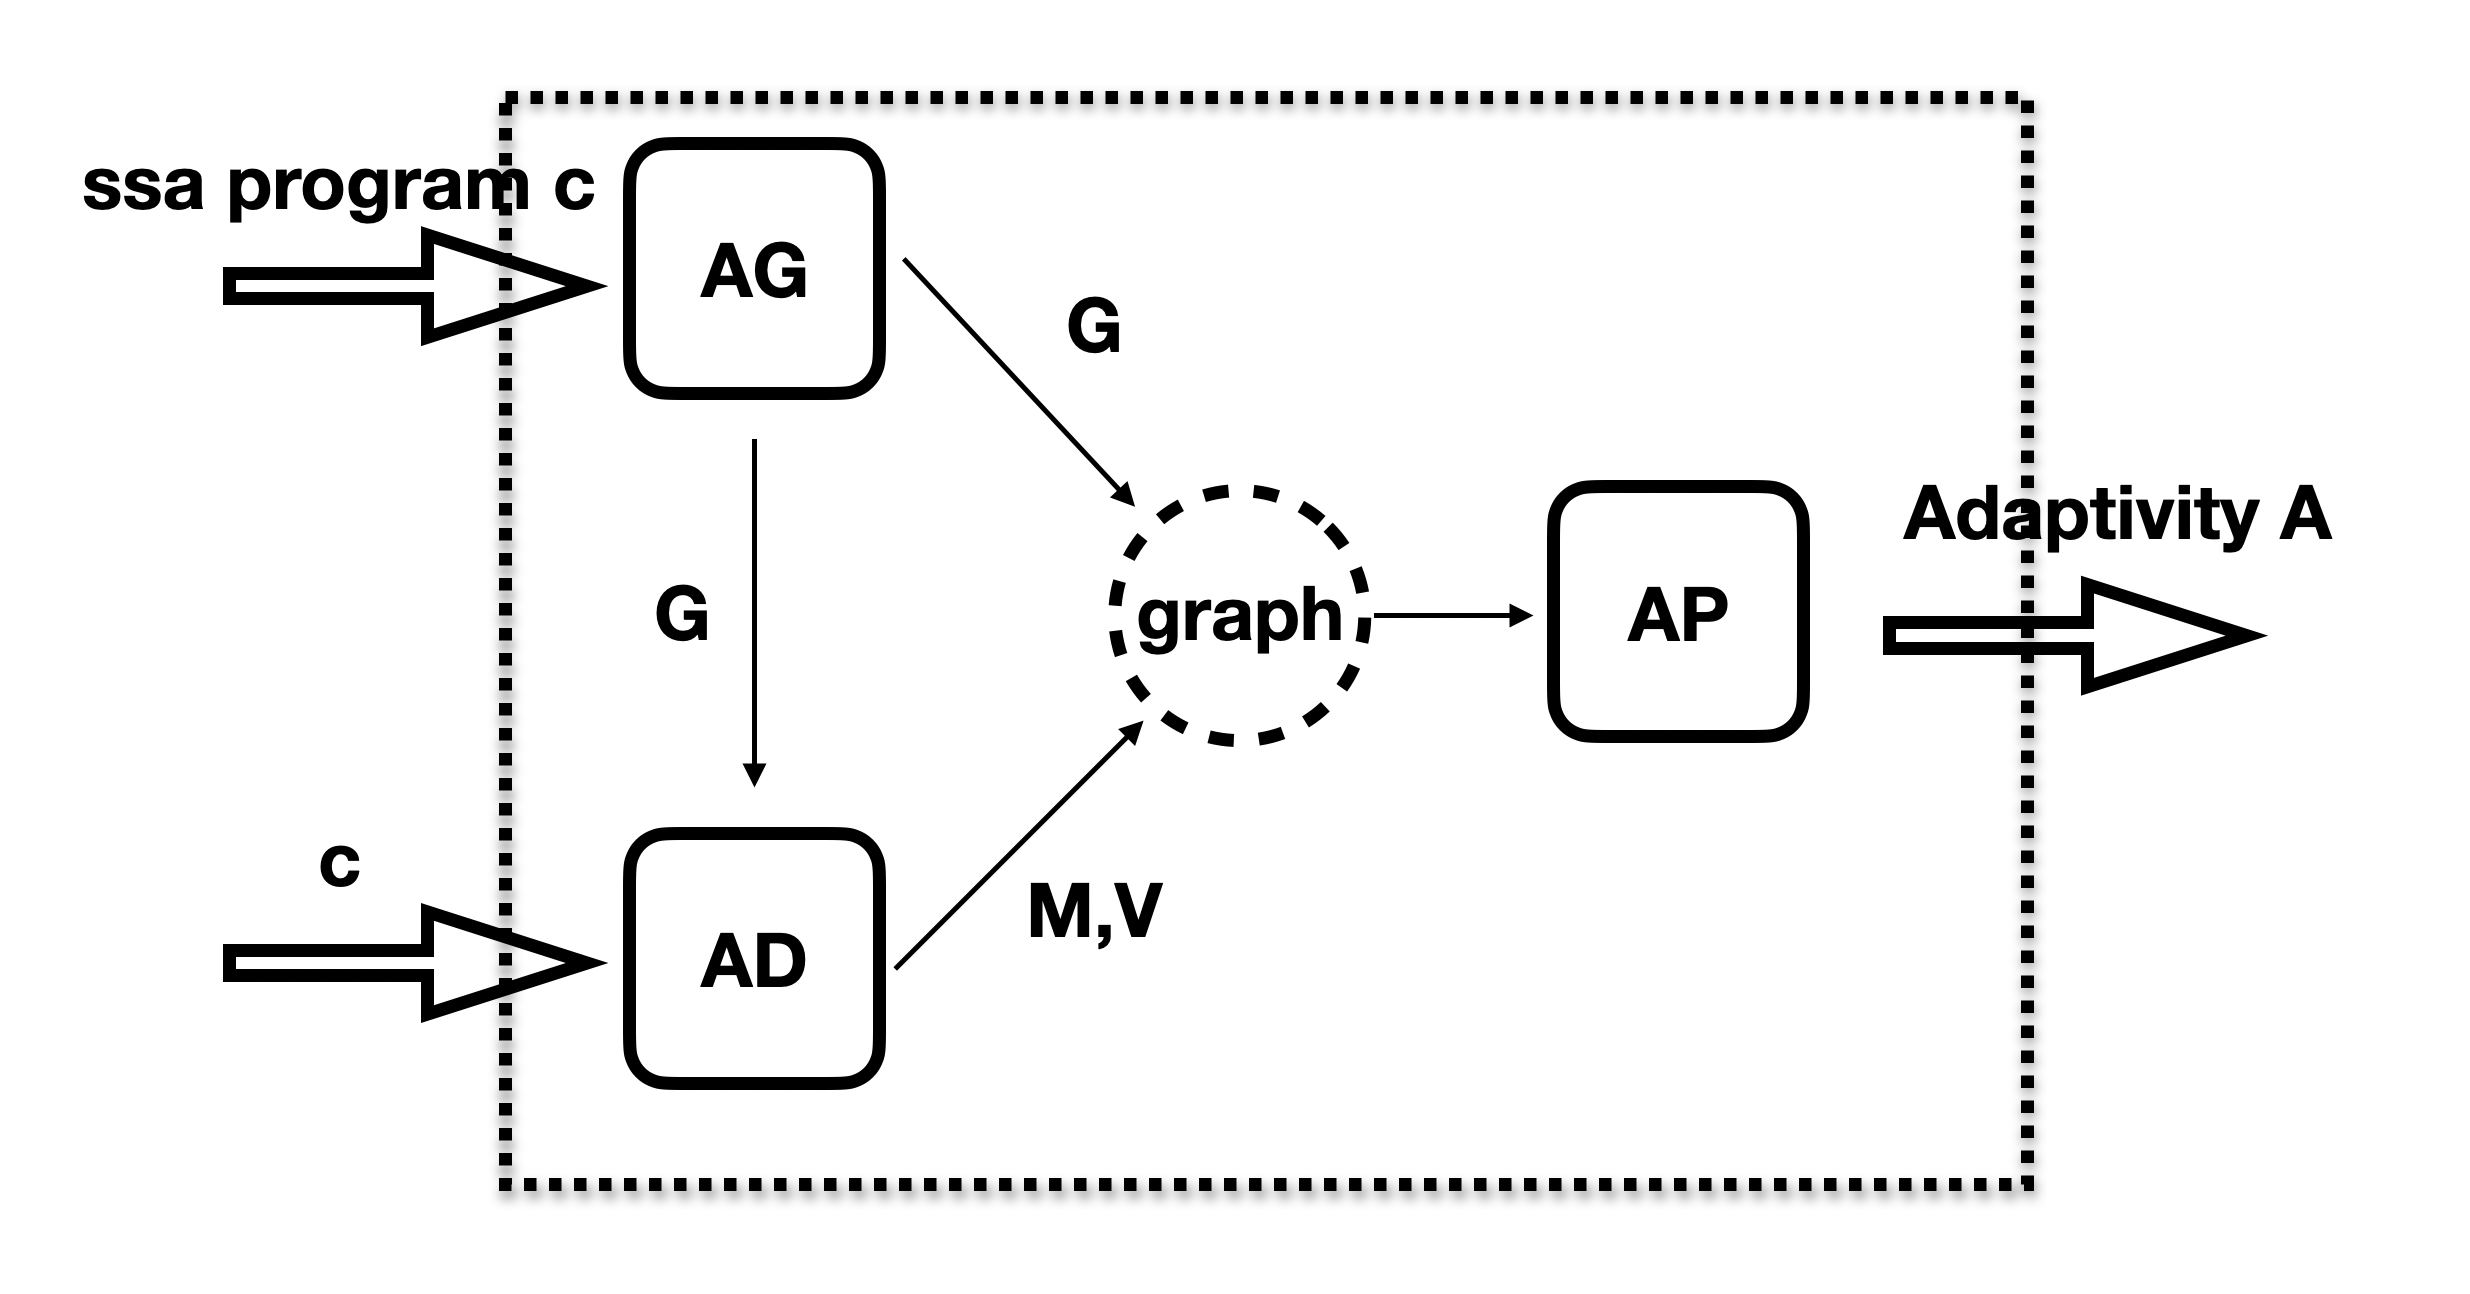
\includegraphics[width=0.7\columnwidth]{adapfun.png}
    \caption{The overview of {\THESYSTEM}}
    \label{fig:adaptfun}
\end{figure}


\subsection{Variable Estimation algorithm}
We first show how $G$ will be collected, through a variable estimating algorithm $\mathsf{AG}$ of the form $\ag{G; w; \ssa{c}}{ G'; w'} $ in Figure~\ref{fig:ag}. The input of $\mathsf{AG}$ is a list of estimated annotated variables $G$ collected before the program $\ssa{c}$, a while map $w$ consistent with previous estimation, a program $\ssa{c}$. The output of the algorithm is the updated global list $G'$, along with the updated while map $w$ for later estimation.   
\begin{figure}
 \begin{mathpar}
\inferrule
{
}
{ \ag{G ;w; \ssa{[\assign {x}{\expr}]^{l}}}{G ++ [\ssa{x}^{(l,w)}];w}
% G ;w; \ssa{[\assign {x}{\expr}]^{l}} \to G ++ [x^{(l,w)}];w 
}
~\textbf{ag-asgn}
\and
\inferrule
{
}
{ \ag{G ;w;  [ \assign{\ssa{x}}{q(\ssa{\expr})}]^{l}}{  G ++ [\ssa{x}^{(l,w)}] ; w} 
}~\textbf{ag-query}
%
\and 
%
\inferrule
{
\ag{G; w; \ssa{c_1}}{  G_1;w_1}
\and 
 \ag{G_1;w ; \ssa{c_2}}{  G_2; w_2}
 \\
 {G_3 = G_2 ++ \ssa{[\bar{x}^{(l,w)}]++ \ssa{[\bar{y}^{(l,w)}]}++ \ssa{[\bar{z}^{(l,w)}]} }}
}
{
\ag{G; w;
[\eif(\ssa{\bexpr},[ \bar{\ssa{x}}, \bar{\ssa{x_1}}, \bar{\ssa{x_2}}] ,[ \bar{\ssa{y}}, \bar{\ssa{y_1}}, \bar{\ssa{y_2}}],[ \bar{\ssa{z}}, \bar{\ssa{z_1}}, \bar{\ssa{z_2}}], \ssa{ c_1, c_2)}]^{l} }{ G_3 ;w}
}~\textbf{ag-if}
%
%
%
\and 
%
\inferrule
{
\ag{G; w; \ssa{c_1}}{ G_1; w_1}
\and 
\ag{G_1;w_1; \ssa{c_2}}{ G_2; w_2}
}
{
\ag{G; w;
\ssa{(c_1 ; c_2)}}{  G_2 ; w_2}
}
~\textbf{ag-seq}
\and 
\inferrule
{
{G_0 = G \quad w_0 =w }
\and
\forall 0 \leq z < N. 
{ \ag{ G_z ++ \ssa{[\bar{x}^{(l, {w_z}+l)}]} ; (w_z+l); \ssa{c}}{ G_{z+1} ; w_{z+1}}  }
\\
{G_f = G_N ++ \ssa{[\bar{x}^{(l, w_N \setminus l)}]} }
\and
{ \ssa{\aexpr} =  {N}  }
}
{\ag{G; w; [\eloop ~ \ssa{\aexpr}, n, [\bar{\ssa{x}}, \bar{\ssa{x_1}}, \bar{\ssa{x_2}}] ~ \edo ~ \ssa{c}]^{l} }{ G_f; w_N\setminus l }
}~\textbf{ag-loop}
% \and 
% \inferrule
% {
% \Gamma \vdash^{(i,i+a )}_{M, V} c 
% }
% {\Gamma \vdash^{(i, i+ N*a)}_{M_{i,a}^N(f), V_{i, a}^N} 
% \ewhile([\bexpr]^l,   c) : \phi \Rightarrow \psi
% }~\textbf{while}
% %
% \and
% %
% \inferrule
% {
% }
% { \ag{ G;w; [ \eswitch(\ssa{\expr}, \ssa{x},(\ssa{v_j} \rightarrow \ssa{q_j} ) )]^{l} } { G ++ [\ssa{x}^{(l, w)}] ; w} }
% ~\textbf{switch}
\end{mathpar}
 \caption{The algorithm $\mathsf{AG}$ }
    \label{fig:ag}
\end{figure}
The assignment is the source of variables $\mathsf{AG}$ estimates, in the case $\textbf{ag-asgn}$ and $\textbf{ag-query}$, the output global list is extended by $\ssa{x}^{(l,w)}$. When it comes to the if command in the rule $\textbf{ag-if}$, variables assigned in the then branch $\ssa{c_1}$, as well as the variables assigned in the else branch $\ssa{c_2}$, and the new generated variables $\bar{\ssa{x}},\bar{\ssa{y}},\bar{\ssa{z}}$ in $ [ \bar{\ssa{x}}, \bar{\ssa{x_1}}, \bar{\ssa{x_2}}] ,[ \bar{\ssa{y}}, \bar{\ssa{y_1}}, \bar{\ssa{y_2}}],[ \bar{\ssa{z}}, \bar{\ssa{z_1}}, \bar{\ssa{z_2}}]$. The sequence is standard by accumulating the predicted variables in the two commands $\ssa{c_1}$ and $\ssa{c_2}$ in a sequence $\ssa{c_1;c_2}$. The loop considers the loop iterations as well by assuming the loop counter $\ssa{\aexpr}$ to be certain natural number $N$ in the rule $\textbf{ag-loop}$. The algorithm counts the assigned variables in every iteration, including those new assigned variables in $\bar{\ssa{x}}$, those variables assigned in the body $\ssa{c}$, with the appropriate annotation showing the iteration number of the variables.      


\subsection{Matrix and Vector based algorithm}
We have a global list $G$ after the first scan of the ssa programs $\ssa{c}$. We develop a matrix and vector based approach based on the global list $G$ to get an estimated upper bound on the adaptivity of the program.  In this approach, a matrix is constructed according to those estimated annotated variables from the global list, in which every row and every column corresponds to the unique variable in $G$ by position. To be precise, in this matrix, $0$ means no dependency while non-zero value in the matrix shows may-dependency between corresponding variables. If the value of $M[i][j]$ in the matrix $M$ is greater than zero, we know annotated variable $G[i]$ may depend on $G[j]$. A vector $V$ has the same size as $G$ and it records whether the corresponding variable $G[i]$ is assigned with a query request. $V[i] =1$ means assigned with a query request and  otherwise $V[i]=0$. We call this algorithm which tracks may-dependency in the ssa programs and query information, $\mathsf{AD}$. The algorithm of the form $ \ad{\Gamma; \ssa{c} ;i }{ M; V;  i' } $, the input is a tuple consisting of three elements: (1) a one-row-N-column matrix $\Gamma$ storing the dependency from previous program, it is used when handling the if command. (2) the ssa program $\ssa{c}$ to be analyzed (3) an index $i$ specifying the location of the first assigned variable of the program $\ssa{c}$ in the global list $G$. The output of $\mathsf{AD}$ also consists of three elements ; (1) A matrix $M$ showing the may-dependency in $\ssa{c}$ (2) A vector $V$ records the query requests in $\ssa{c}$ (3) the index $i'$ that refers to the next position of the last assigned variable in $\ssa{c}$, if exists. The existence of the index $i'$ helps to locate the first assigned variable if we need to analyze programs after $\ssa{c}$.  

We first define some functions which use the indices in $G$. 
The function $\mathsf{L(i)}$ generates one-column-N-rows  matrix, where only the $i-th$ row is $1$ and all the other rows are $0$. This function is used to locate the right row when calculate the matrix when analyzing assignment and query. 

The function $\mathsf{R(e, i)}$ generates a one-row-N-column matrix. For every variable used in $e$, it finds the corresponding index $i$ in $G$ so that $G[i]$ maps to the variable and mark the $i$th column as $1$. If it is not found, we do not mark. When we say $G[i]$ maps to a target variable, we take off the annotation of $G[i]$ and check if the left variable is the same as the target variable. To handle loop, for instance, a variable $y$ appears many times in $G$, but with different annotations(iteration numbers), the argument $i$ helps to find most recent assignment variable $y$ before the index $i$ in $G$. It is still used when analyzing assignment and query. Thanks to our ssa language, our choice of the most recent assigned variable is reasonable because the variable used in the loop refers to the most recent assignment and every variable is uniquely assigned in its ssa form. 

We define $M_1;M_2$ to combine two matrix, where $M_1 + M_2$ is the standard sum of two matrix.
\[
M_1 ; M_2  :=  M_2 \cdot M_1 + M_1 + M_2 
\]
And define the operator $\uplus$ to combine two vectors.
\[
V_1 \uplus V_2  :=  \left\{
\begin{array}{ll}
1 & (V_1[i] = 1 \lor V_2[i] = 1) \land i = 1, \cdots, N \land |V_1| = |V_2|\\
0 & o.w.
\end{array}\right.
\]
For the sake of brevity, we also define some annotations as follows. We show how the algorithm $\mathsf{AD}$ handles the extra part $[ \bar{\ssa{x}}, \bar{\ssa{x_1}},\bar{\ssa{x_2}} ] $ in the if and loop commands. First, we give a unique name for variables in lists $\bar{\ssa{x}}, \bar{\ssa{x_1}}, \bar{\ssa{x_2}}$ respectively, as follows: {$ \forall 0 \leq z < |\bar{\ssa{x}}|. \bar{\ssa{x}}(z) = \ssa{x_z}, \bar{\ssa{x_1}}(z) = \ssa{x_{1z}}, \bar{\ssa{x_2}}(z) = \ssa{x_{2z}} $ }. And then we treat every tuple $(\ssa{x_z},\ssa{x_{1z}},\ssa{x_{2z}} )$ in $[\bar{\ssa{x}}, \bar{\ssa{x_1}}, \bar{\ssa{x_2}} ]$ as the simple may dependency case : $\ssa{x_z}$ may depend on both $ \ssa{x_{1z}}$ and $\ssa{x_{2z}}$, just like $ \assign{\ssa{x_z} }{\ssa{x_{1z}} + \ssa{x_{2z}} }$, defined as follows. 
$
 \ad{\Gamma; [\bar{\ssa{x}}, \bar{\ssa{x_1}}, \bar{\ssa{x_2}} ] ; i }{ M; V_{\emptyset}; i + |\bar{\ssa{x}}| } 
  \triangleq { \forall 0 \leq z < |\bar{\ssa{x}}|.
  \ad{\Gamma;\assign{\ssa{x_z} }{\ssa{x_{1z}} + \ssa{x_{2z}} }; i+z }{ M_{x_z};  V_{\emptyset}; i+z+1} }$
   where $M = \sum_{o \leq z < |\bar{\ssa{x}}| }M_{x_z} $.
% \framebox{$ \ad{\Gamma; \ssa{c} ; i_1){M;V;i_2} $}
%
\begin{figure}
\begin{mathpar}
\inferrule
{M = \mathsf{L}(i) * ( \mathsf{R}(\ssa{\expr},i) + \Gamma )
}
{
 \ad{\Gamma;[\assign {\ssa{x}}{\ssa{\expr}} ]^{l}; i }{M; V_{\emptyset}; i+1 }
% \Gamma \vdash_{M, V_{\emptyset}}^{(i, i+1)} [\assign {\ssa{x}}{\ssa{\expr}} ]^{l}
}
~\textbf{ad-asgn}
\and
\inferrule
{M = \mathsf{L}(i) * ( \mathsf{R}(\ssa{\expr},i) + \Gamma )
\\
V= \mathsf{L}(i)
}
{ 
\ad{\Gamma;[ \assign{\ssa{x}}{q(\ssa{\expr})} ]^{l} ; i }{M;V;i+1}
%  \vdash^{(i, i+1)}_{M, V} [ \assign{\ssa{x}}{q(\ssa{\expr})} ]^{l} 
}~\textbf{ad-query}
%
\and 
%
\inferrule
{
{\ad{\Gamma + \mathsf{R}(\ssa{\bexpr}, i_1); \ssa{c_1} ; i_1 }{ M_1;V_1;i_2 }}
% \Gamma + \mathsf{R}(\bexpr, i_1) \vdash^{(i_1, i_2)}_{M_1, V_1} \ssa{c_1} 
% : \Phi \land \bexpr \Rightarrow \Psi
\and 
{\ad{\Gamma + \mathsf{R}(\ssa{\bexpr}, i_1);\ssa{c_2} ; i_2 }{ M_2; V_2 ;i_3}}
% \Gamma + \mathsf{R}(\ssa{\bexpr}, i_1) \vdash^{(i_2, i_3)}_{M_2, V_2} \ssa{c_2} 
% : \Phi \land \neg \bexpr \Rightarrow \Psi
\\
% { \forall 0 \leq j < |\bar{x}|. \bar{x}(j) = x_j, \bar{x_1}(j) = x_{1j}, \bar{x_2}(j) = x_{2j}  }
{\ad{\Gamma; [ \bar{\ssa{x}}, \bar{\ssa{x_1}}, \bar{\ssa{x_2}}]; i_3 }{ M_x; V_{\emptyset}; i_3+|\bar{\ssa{x}}| }}
%
\and
%
{\ad{\Gamma; [ \bar{\ssa{y}}, \bar{\ssa{y_1}}, \bar{\ssa{y_2}}]; i_3+|\bar{\ssa{x}}| }{ M_y; V_{\emptyset}; i_3+|\bar{\ssa{x}}|+|\bar{\ssa{y}}| }}
%
\\
%
{\ad{\Gamma; [ \bar{\ssa{z}}, \bar{\ssa{z_1}}, \bar{\ssa{z_2}}]; i_3+|\bar{\ssa{x}}|+ |\bar{\ssa{y}}|}{ M_y; V_{\emptyset}; i_3+|\bar{\ssa{x}}|+|\bar{\ssa{y}}| + |\bar{\ssa{z}}| }}
% { \forall 0 \leq j < |\bar{x}|.  \Gamma \vdash_{M_{x_j}, V_{\emptyset}}^{i_3+j, i_3+j+1 } x_j \leftarrow x_{1j} + x_{2j} }
% \and
% { \forall 0 \leq j < |\bar{y}|.  \Gamma \vdash_{M_{y_j}, V_{\emptyset}}^{i_3+|\bar{x}|+j, i_3+|\bar{x}|+j+1 } y_j \leftarrow y_{1j} + y_{2j} }
% \\
% { \forall 0 \leq j < |\bar{z}|.  \Gamma \vdash_{M_{z_j}, V_{\emptyset}}^{i_3+|\bar{x}|+|\bar{y}|+j, i_3+|\bar{x}|+|\bar{y}|+j+1 } z_j \leftarrow z_{1j} + z_{2j} }
\\
{M = (M_1+M_2)+ M_x+M_y +M_z }
}
{
\Gamma \vdash^{(i_1, i_3+|\bar{x}|+|\bar{y}|+|\bar{z}|)}_{M, V_1 \uplus V_2 } 
[\eif(\ssa{\bexpr},[ \bar{\ssa{x}}, \bar{\ssa{x_1}}, \bar{\ssa{x_2}}] ,[ \bar{\ssa{y}}, \bar{\ssa{y_1}}, \bar{\ssa{y_2}}] , [ \bar{\ssa{z}}, \bar{\ssa{z_1}}, \bar{\ssa{z_2}}] , \ssa{ c_1, c_2)}]^{l}
}~\textbf{ad-if}
%
%
%
\and 
%
\inferrule
{
{\ad{\Gamma; \ssa{c_1} ; i_1 }{ M_1 ; V_1; i_2 }  }
% \Gamma \vdash^{(i_1, i_2)}_{M_1, V_1} \ssa{c_1} 
% : \Phi \Rightarrow \Phi_1
\and 
{\ad{\Gamma;\ssa{c_2}; i_2}{M_2; V_2 ;i_3 }}
% \Gamma \vdash^{(i_2, i_3)}_{M_2, V_2} \ssa{c_2} 
% : \Phi_1 \Rightarrow \Psi 
}
{
\ad{\Gamma ; (\ssa{c_1 ; c_2} ) ; i_1}{(M_1 {;} M_2) ; V_1 \uplus V_2 ; i_3  }
% \Gamma \vdash^{(i_1, i_3)}_{M_1 {;} M_2, V_1 \uplus V_2}
% \ssa{c_1 ; c_2} 
% : \Phi \Rightarrow \Psi
}
~\textbf{ad-seq}
\and 
\inferrule
{
B= |\ssa{\bar{x}}| \and {A = |\ssa{c}|}
% \and
% {\Gamma \vdash^{(i, i+B)}_{M_{10}, V_{10}} [\bar{\ssa{x}}, \bar{\ssa{x_1}}, \bar{\ssa{x_2}}] }
% \and
% {\Gamma \vdash^{(i+B,i+B+A )}_{M_{20}, V_{20}} \ssa{c} 
% }
\\
\forall 0 \leq j < N. 
{\ad{\Gamma;[\bar{\ssa{x}}, \bar{\ssa{x_1}}, \bar{\ssa{x_2}}]; i+ j*(B+A) }{M_{1j};V_{1j}; i+B+j*(B+A) }}
% {\Gamma \vdash^{(i+j*(B+A), i+B+j*(B+A))}_{M_{1j}, V_{1j}}  } [\bar{\ssa{x}}, \bar{\ssa{x_1}}, \bar{\ssa{x_2}}]
\\
{
\ad{\Gamma;\ssa{c} ; i+B+j*(B+A)  }{M_{2j}; V_{2j}; i+B+A+j*(B+A) }
% \Gamma \vdash^{(i+B+j*(B+A),i+B+A+j*(B+A) )}_{M_{2j}, V_{2j}} \ssa{c} 
% : \Phi \land e_n = \lceil{z+1}\rceil \Rightarrow \Psi 
}
\\
{
\ad{\Gamma ; [\bar{\ssa{x}}, \bar{\ssa{x_1}}, \bar{\ssa{x_2}}] ; i+N*(B+A) }{M; V ;i+N*(B+A)+B}
% \Gamma \vdash^{(i+N*(B+A) ,i+N*(B+A)+B )}_{M, V} [\bar{\ssa{x}}, \bar{\ssa{x_1}}, \bar{\ssa{x_2}}]
% : \Psi \Rightarrow \Phi \land e_N = \lceil{z}\rceil 
}
\\
{ \ssa{\aexpr} =  {N}  }
\and
{M' = M+ \sum_{0 \leq j <N}( M_{1j}+M_{2j})  }
\and
{V' = V \uplus \sum_{0 \leq j <N}( V_{1j} \uplus V_{2j})  }
}
{\Gamma \vdash^{(i, i+N*(B+A)+B   )}_{M', V'} 
[\eloop ~ \ssa{\aexpr}, 0, [\bar{\ssa{x}}, \bar{\ssa{x_1}}, \bar{\ssa{x_2}}] ~ \edo ~ \ssa{c}]^{l}
% : \Phi \land \expr_N = \lceil { N} \rceil \Rightarrow \Phi \land \expr_N = \lceil{0}\rceil
}~\textbf{ad-loop}
% \and 
% \inferrule
% {
% \Gamma \vdash^{(i,i+a )}_{M, V} c 
% }
% {\Gamma \vdash^{(i, i+ N*a)}_{M_{i,a}^N(f), V_{i, a}^N} 
% \ewhile([\bexpr]^l,   c) : \phi \Rightarrow \psi
% }~\textbf{while}
% %
% \and
% %
% \inferrule
% { \Gamma + \mathsf{R}(\expr,i) \vdash^{(i, i+1)}_{M, V} \assign{ x}{q_j} 
% % : \Phi \Rightarrow \Psi
% \\
% j \in \{1, \dots, N\}     }
% {\Gamma \vdash^{(i, i+1)}_{ M,V } 
% [\eswitch(\ssa{\expr}, \ssa{x},(v_j \rightarrow q_j ) ]^{l}
% % : \Phi \Rightarrow \Psi 
% }
% ~\textbf{switch}
% %
% \and
% %
% \inferrule
% { 
% \vDash 
% \Phi \Rightarrow \Phi'  
% \and
% \Gamma \vdash^{(i_1, i_2)}_{(M',V')} c : \Phi' \Rightarrow \Psi'
% \and
% \vDash \Psi' \Rightarrow \Psi
% \and 
% \Phi \vDash M' \leq M
% \and 
% \Phi \vDash V' \leq V
% }
% {\Gamma \vdash^{(i_1, i_2)}_{(M,V)} c 
% : \Phi \Rightarrow \Psi
% }
% ~\textbf{conseq}
\end{mathpar}
    \caption{The algorithm AD}
    \label{fig:algo_ad}
\end{figure}
One of the key idea under algorithm $\mathsf{AD}$ is to track the indices $i$,$i'$ both in the input and output to synchronize with its previous algorithm $\mathsf{AG}$. The index in $\mathsf{AD}$ increases as the same way as the global list expands after the analysis of a program $\ssa{c}$, which helps $\mathsf{AD}$ record the dependency relation from the program $\ssa{c}$ in the right place of the matrix. For example, in the case $\textbf{ad-asgn}$ and $\textbf{ad-query}$, the index increases by 1, which corresponds to their counterparts of algorithm $\textbf{AG}$. The if and loop commands have the extra part $ [\bar{\ssa{x}}, \bar{\ssa{x_1}}, \bar{\ssa{x_2}}] $ and we find that the output index increases by also considering this part as we do in collecting the global list.  

Another interesting point is the construction of the matrix. The fundamental case is the assignment and query cases. We use a function $L(i)$ to generate a N-row-one-column matrix $L$ to guarantee the resulting matrix only has non-zeros at row $i$. The intuition behind is that one single assignment or query request can only reveal the dependency of its assigned variable (corresponding to one row of the matrix) to the variables used on the right hand sides. Thanks to the index $i$, we know which row this assignment should be in the matrix. The function $\mathsf{R}(\ssa{\expr},i)$ gets a one-row-N-column matrix marking the variables used in the right hand side. The $\Gamma$ is designed for the if command and we will discuss it later. We can see one simple example $sa$ to get a taste.     
\[
sa \triangleq
\begin{array}{l}
    \left[x_1 \leftarrow 2 \right]^1; \\
    \left[x_2 \leftarrow x_1 + 2 \right]^2 ; \\
    \left[x_3 \leftarrow x_1 + x_2 \right]^3
\end{array}
\]
In the program $sa$, only simple assignment is involved. When we assume $\Gamma$ is empty, for the assignment at line $3$, the matrix is built as follows.
\[
\textbf{line3:} ~~
 \left[x_3 \leftarrow x_1 + x_2 \right]^3 :
 ~~~
\begin{blockarray}{cc}
\begin{block}{c[c]}
 x_1 & 0   \\
 x_2 & 0 \\
 x_3 & 1 \\
\end{block}
\end{blockarray}
*
\begin{blockarray}{ccc}
x_1 & x_2 & x_3 \\
\begin{block}{[ccc]}
1 & 1 & 0 \\
\end{block}
\end{blockarray}
= 
\begin{blockarray}{cccc}
& x_1 & x_2 & x_3\\
\begin{block}{c[ccc]}
x_1 & 0 & 0 & 0 \\
x_2 & 1 & 0 & 0 \\
x_3 & 1 & 1 & 0 \\
\end{block}
\end{blockarray}
\]
% a simple example of assignment
% \begin{example}[Simple Assignment]
% \[
% SA \triangleq
% \begin{array}{l}
%     \left[x_1 \leftarrow 2 \right]^1; \\
%     \left[x_2 \leftarrow x_1 + 2 \right]^2 ; \\
%     \left[x_3 \leftarrow x_1 + x_2 \right]^3
% \end{array}
% \]
% %
% %
% \[
%  \textbf{line2:} ~~
%  \left[x_2 \leftarrow x_1 + 2 \right]^2 :
%  ~~~
% \begin{blockarray}{cc}
% \begin{block}{c[c]}
%  x_1 & 0   \\
%  x_2 & 1 \\
%  x_3 & 0 \\
% \end{block}
% \end{blockarray}
% *
% \begin{blockarray}{ccc}
% x_1 & x_2 & x_3 \\
% \begin{block}{[ccc]}
% 1 & 0 & 0 \\
% \end{block}
% \end{blockarray}
% = 
% \begin{blockarray}{cccc}
% & x_1 & x_2 & x_3\\
% \begin{block}{c[ccc]}
% x_1 & 0 & 0 & 0 \\
% x_2 & 1 & 0 & 0 \\
% x_3 & 0 & 0 & 0 \\
% \end{block}
% \end{blockarray}
% \]
% %
% %
% %
% \[
% \textbf{line3:} ~~
%  \left[x_3 \leftarrow x_1 + x_2 \right]^3 :
%  ~~~
% \begin{blockarray}{cc}
% \begin{block}{c[c]}
%  x_1 & 0   \\
%  x_2 & 0 \\
%  x_3 & 1 \\
% \end{block}
% \end{blockarray}
% *
% \begin{blockarray}{ccc}
% x_1 & x_2 & x_3 \\
% \begin{block}{[ccc]}
% 1 & 1 & 0 \\
% \end{block}
% \end{blockarray}
% = 
% \begin{blockarray}{cccc}
% & x_1 & x_2 & x_3\\
% \begin{block}{c[ccc]}
% x_1 & 0 & 0 & 0 \\
% x_2 & 1 & 0 & 0 \\
% x_3 & 1 & 1 & 0 \\
% \end{block}
% \end{blockarray}
% \]
% %
% \end{example}
 We use a one-row-N-column matrix $\Gamma$ as one of the input of $\mathsf{AD}$, to handle the cases when the control flow diverges in the labelled if command $[\eif(\ssa{\bexpr},[ \bar{\ssa{x}}, \bar{\ssa{x_1}}, \bar{\ssa{x_2}}] ,[ \bar{\ssa{y}}, \bar{\ssa{y_1}}, \bar{\ssa{y_2}}] , [ \bar{\ssa{z}}, \bar{\ssa{z_1}}, \bar{\ssa{z_2}}] , \ssa{ c_1, c_2)}]^{l} $, where the execution of either branch may depend on the conditional guard $\ssa{\bexpr}$. Follow this intuition, the analysis of either branch is supposed to consider the variables used in the conditional $\ssa{\bexpr}$, tracked in $\Gamma$. In the case $\textbf{ad-if}$, we can see the analysis of the two branches $\ssa{c_1}$ and $\ssa{c_2}$ share the same input $\Gamma + \mathsf{R}(\ssa{\bexpr}, i)$ and $\mathsf{R}(\ssa{\bexpr}, i) $ tells the variables assigned before the if command and used in the conditional $\ssa{\bexpr}$.   

We compose the matrix and vectors in the case of sequence in $\textbf{ad-seq}$. The non-zeros or we call it effect range of the matrix and vector is decided by its input and output indices. From the case $\textbf{ad-seq}$, two programs $\ssa{c_1}$ and $\ssa{c_2}$ have disjoint effect ranges $[i_1, i_2)$ and $[i_1,i_3)$, it is safe to combine them without lose information. 

The loop case is handled in a well organized way. We use $B= |\bar{\ssa{x}}|$ and $A= |{\ssa{c}}|$ to estimate the size of variables assigned in $\bar{\ssa{x}}$ and $\ssa{c}$. And  $|\ssa{c}|$ is defined by the help of the algorithm $\mathsf{AG}$, defined as $|\ssa{c}|= |G|$ when $\ag{[];\ssa{c};\emptyset }{ G; \emptyset }$. The algorithm then gets how many iterations $N$ the loop may executes from the loop counter $\ssa{\aexpr}$. For every iteration, it first records the dependency relations between variables in $ [\bar{\ssa{x}}, \bar{\ssa{x_1}}, \bar{\ssa{x_2}}]$ by constructing a corresponding matrix $M_{1j}$ ($j$ is the iteration number) and an empty vector $V_{1j}$, and analyze the loop body $\ssa{c}$ with a resulting matrix $M_{2j}$ and vector $V_{2j}$. We give an extra analysis of those new assigned variables as what $\mathsf{AG}$ does, it works well when the loop is executed ($N = 0$) or not. We know that for all the possible iteration number $j$, $M_{1j}$ and $M_{2j}$ have disjoint effect ranges so we combine them, similar as the vectors $V_{1j}$ and $V_{2j}$.   

Finally, we are able to construct a variable-based weighted dependency graph based on $G$,$M$ and $V$ generated by the framework. The definition of the estimated adaptivity is the weight of the most weighted path in the graph defined as follows. 

\begin{defn}
[Estimated Adaptivity]
Given a program $\ssa{c}$, the global list $G$, and $\ad{\Gamma; \ssa{c}; i_1}{M, V, i_2}$, the weighted dependency graph $G_{ssa}(M, V,G,i_1,i_2) = (Nodes, Edges, Weights)$ is defined as:
\\
Nodes $Vt = \{ G(j) \in \mathcal{LV} \mid i_1 \leq j < i_2 \}$
\\
Edges $E = \{ (G(j_1), G(j_2)) \in \mathcal{LV} \times \mathcal{LV} \mid M[j_1][j_2] \geq 1 \land  i_1 \leq j_1,j_2 < i_2   \}$
\\
 Weights $Wt = \{ (  G(j), 1 ) \in \mathcal{LV} \times \mathcal{N} | i_1 \leq j < i_2 \land V[j] = 1\}
        \cup \{ (  G(j), 0 ) \in \mathcal{LV} \times \mathcal{N} | i_1 \leq j < i_2 \land V[j] = 0 \} $.
        
Adaptivity of the program defined according to the graph is as:
\[
Adapt(M, V,i_1,i_2) := \max_{vt_1, vt_2 \in Vt}\{ \mathsf{Weight}( p(vt_1, vt_2), Wt) \},
\]
where $p(k, l)$ is the path in graph $G_{ssa}(M, V, i_1,i_2)$ starting from $k$ to $l$, $\mathsf{Weight}(p(vt_1,vt_2), Wt)$ get the total sum of weights along the path $p(vt_1,vt_2)$.
\end{defn}        

\subsection{Analysis on two round algorithm}
We show how {\THESYSTEM} analyze the two round algorithm. For the sake of brevity, we conduct the analysis on the simplified two round algorithm $TR^{ssa}$.

% \[
% TR^{ssa}(k) \triangleq
% {
% \begin{array}{l}
%     % \left[j \leftarrow 0 \right]^1 ; \\
%     \clabel{a_1 \leftarrow []}^{1} ; \\
%     \clabel{\assign{j_1}{0} }^{2} ; \\
%     \eloop ~ \clabel{k}^{3} ~ \edo [(j_3, j_1,j_2),(a_3, a_1,a_2)]~ \\
%     \Big(
%     \clabel{ x_1 \leftarrow q(\chi(j_3)\cdot \chi(k))}^{4}  ; \\
%     \clabel{ \assign{j_2}{j_3+1} }^{5} ;\\
%     \clabel{a_2 \leftarrow x_1 :: a_3}^{6}       \Big);\\
%     \clabel{l_1 \leftarrow q(\mathrm{sign}\big (\sum_{i\in [k]} \chi(i)\times\ln\frac{1+a_3[i]}{1-a_3[i]} \big ))}^{7}\\
% \end{array}
% }
% \]
{\THESYSTEM} first runs the algorithm $\mathsf{AG}$ to generate the global list $G$. We assume the input $k=2$ and have the following.

\[G_{k=2} = \left[
  {a_1}^{(1,\emptyset)} , {a_3}^{(2,[2:1])} , {x_1}^{(3,[2:1])} , {a_2}^{(4,[2:1])} ,  {a_3}^{(2,[2:2])} , {x_1}^{(3,[2:2])} , {a_2}^{(4,[2:2])} , {a_3}^{(2,\emptyset)} , {l_1}^{(5,\emptyset)}   \right] \]
% \[G_{k=2} = \left[ \begin{array}{l}
%      {a_1}^{(1,\emptyset)} , {j_1}^{(2,\emptyset)}, {j_3}^{(3,[2:1])} , {a_3}^{(3,[2:1])} , {x_1}^{(4,[2:1])} ,{j_2}^{(5,[2:1])} ,
%   {a_2}^{(6,[2:1])},  \\
%     {j_3}^{(3,[2:2])} , {a_3}^{(3,[2:2])} , {x_1}^{(4,[2:2])} ,{j_2}^{(5,[2:2])} ,
%   {a_2}^{(6,[2:2])},
%   {j_3}^{(3,\emptyset)} , {a_3}^{(3,\emptyset)} ,
%   {l_1}^{(7,\emptyset)} \\  
% \end{array}
%      \right] \]
 We denote $a_1^{1}$ short for ${a_1}^{(1,\emptyset)}$ and ${a_3}^{(2,1)}$ short for ${a_3}^{(2,[2:1])}$. Then the resulting matrix $M_{tr}$ and $V_{tr}$ of the algorithm $\mathsf{AD}$ as follows.
 
{ \tiny
 \[
M_{tr} =  \left[ \begin{matrix}
 & a_1^{1} & a_3^{(2,1)} & x_1^{(3,1)} & a_2^{(4,1)}  & a_3^{(2,2)} & x_1^{(3,2)} & a_2^{(4,2)} & a_3^{2} & l_1^{5}\\
 a_1^{1} & 0 & 0 & 0 & 0 & 0 & 0 & 0 &0 &0 \\
a_3^{(2,1)} & 1 & 0 & 0 & 0 & 0 & 0 & 0&0&0\\
x_1^{(3,1)} & 0 & 0 & 0 & 0 & 0 & 0& 0& 0 &0\\
a_2^{(4,1)} & 0 & 1 & 1 & 0 & 0 & 0 & 0& 0&0\\
a_3^{(2,2)} & 1 & 0 & 0 & 1 & 0 & 0 & 0 & 0&0 \\
x_1^{(3,2)} & 0 & 0 & 0 & 0 & 0 & 0 & 0& 0&0\\
a_2^{(4,2)} & 0 & 0 & 0 & 0 & 1 & 1 & 0& 0&0\\
a_3^{2} & 1 & 0 & 0 & 0 & 0 & 0 & 1& 0&0\\
l_1^{5} & 0 & 0 & 0 & 0 & 0 & 0 & 0 & 1 &0 \\
 \end{matrix} \right] 
~ , V_{tr} = \left [ \begin{matrix}
a_1^{1} &  0 \\
a_3^{(2,1)} & 0 \\
x_1^{(3,1)} & 1 \\
a_2^{(4,1)} &  0 \\
a_3^{(2,2)} & 0 \\
x_1^{(3,2)} & 1 \\
a_2^{(4,2)} &  0 \\
a_3^{2} &  0 \\
l_1^{5} &  1 \\
\end{matrix} \right ]
\]
}
%% a graph is better here

\subsection{ Soundness of {\THESYSTEM}}
We would like to show that the query-based dependency graph generated from the trace of the execution of the target ssa program is a subgraph of the variable-based dependency graph predicted from our algorithm ${\THESYSTEM}$, and the query requested during the execution is also bounded by an estimation from our algorithm.

We first give a definition of subgraph of a query-based dependency graph with respect to a variable-based dependency graph.
\begin{defn}
[Subgraph]
Given a query-based dependency graph $G_{s} = (V_1, E_1)$, a variable-based dependency graph $G_{ssa} = (V_2, E_2)$, $G_{s} \subseteq G_{ssa}$ iff:\\
$\exists f$ so that \\
1. for every $v \in V_1$, $f(v) \in V_2$. 
\\
2. $\forall e=(v_i, v_j) \in E_1$, there exists a path 
% $g(e)$ 
from $f(v_i)$ to $f(v_2)$ in $G_{ssa}$.
\end{defn}

Then we show the soundness of {\THESYSTEM}. In the theorem, we use some definition. $G \vDash M, V$ says that $G$ and $M$, $V$ have the corresponding size. $G; w \vDash (\ssa{c}, i_1,i_2)$ checks if the variables assigned in $\ssa{c}$ calculated by $\mathsf{AG}$ matches the variables in $G$ from index $i_1$ to $i_2$.

\begin{thm}
[Soundness of {\THESYSTEM}]
Given $ \ad{\Gamma; \ssa{c}; i_1 }{M; V;i_2}$,  for any global list $G$,  loop maps $w$ such that $G ;w \vDash (\ssa{c}, i_1, i_2) \land G \vDash (M,V)$. $K$ is the number of queries inquired during the execution of the piece of program $\ssa{c}$ and |V| gives the number of non-zeros in $V$. 
% $|.|_{low} $ is the annotation erasure, which turns a ssa form program $\ssa{c}$ to its low-level version.
Then,
\[
K \leq |V| \land \forall D, \ssa{m}. G_{s}(\ssa{c},D,\ssa{m},w) \subseteq G_{ssa}(M, V,G,i_1, i_2)
\]      
\end{thm}


\section{More examples}
The two round strategy works well in our framework, we explore further to look at an advanced adaptive data analysis algorithm - multiple round algorithm.
\begin{example}[Two Round Algorithm]
    \[
    %
        \bf{TRC}(k) \triangleq
    \begin{array}{l}
           \clabel{ a \leftarrow []}^{1} ; \\
            \clabel{\assign{j}{k} }^{2} ; \\
            \ewhile ~ \clabel{j > 0}^{3} ~ \edo ~ \\
            \Big(
             \clabel{x \leftarrow (\chi(k - j)\cdot \chi(k)) }^{4}  ; \\
             \clabel{\assign{j}{j-1}}^{5} ;\\
            \clabel{a \leftarrow x :: a}^{6}       \Big);\\
            \clabel{l \leftarrow (\mathrm{sign}\big (\sum_{i\in [k]} \chi(i)\times\ln\frac{1+a[i]}{1-a[i]} \big ))}^{7}\\
        \end{array}
    \]
    %
    \begin{algorithm}
    \footnotesize
    \caption{A two-round analyst strategy for random data (The example in  \cite{dwork2015preserving})}
    \label{alg:twoRound}
    \begin{algorithmic}
    \REQUIRE Mechanism $\mathcal{M}$ with a hidden state $X\in [N]^{n}$ sampled u.a.r., control set size $c$
    % \STATE Define control dataset $C = \{0,1, \cdots, c - 1\}$
    % \STATE Initialize $Nscore(i) = 0$ for $i \in [N]$, $I = \emptyset$ and $Cscore(C(i)) = 0$ for $i \in [c]$
    % \STATE  {\bf for}\ $j\in [k]$\ {\bf do} 
    % \STATE \qquad {\bf let} $p=\uniform(0,1)$ 
    % \STATE \qquad {\bf define} $q (x) = \bernoulli ( p )$ .
    % \STATE \qquad {\bf define} $qc (x) = \bernoulli ( p )$ .
    % \STATE \qquad {\bf let} $a = \mathcal{M}(q)$ 
    % \STATE \qquad {\bf for}\ $i \in [N]$\ {\bf do}
    % \STATE \qquad \qquad $Nscore(i) = Nscore(i) + (a - p)*(q (i) - p)$ if $i \notin I$
    % \STATE \qquad {\bf for}\ $i \in [c]$\ {\bf do}
    % \STATE \qquad \qquad $Cscore(C(i)) = Cscore(C(i)) + (a - p)*(qc (i) - p)$
    % \STATE \qquad {\bf let} $I = \{i | i\in [N] \land Nscore(i) > \max(Cscore)\}$
    % \STATE \qquad {\bf let} $X = X \setminus I$ 
    \RETURN $X$.
    % \ENSURE 
    \end{algorithmic}
    \end{algorithm}
    %
%
    \end{example}

\begin{example}[Multiple Round Algorithm]
%
\[
%
MR(k) \triangleq
\begin{array}{l}
     \left[j \leftarrow k \right]^1 ; \\
    \left[I_1 \leftarrow [] \right]^2; \\
    \ewhile ~ \clabel{j > 0}^{3} ~ \edo ~ \\
    \Big(
    \clabel{\assign{j}{j-1}}^{4} ;\\
    \left[p_1 \leftarrow c \right]^5; \\
    \left[ a_1 \leftarrow q (p, I_3) \right]^6;\\
    \left[I_2 \leftarrow \mathrel{\mathsf{update}} ( {I_3}, (a_1, p_1))  \right]^7
    \Big) 
\end{array}
\]
%
\begin{algorithm}
\footnotesize
\caption{A multi-round analyst strategy for random data base \cite{dwork2015preserving}}
\label{alg:multiRound}
\begin{algorithmic}
\REQUIRE Mechanism $\mathcal{M}$ with a hidden state $X\in [N]^{n}$ sampled u.a.r., control set size $c$
\STATE Define control dataset $C = \{0,1, \cdots, c - 1\}$
\STATE Initialize $Nscore(i) = 0$ for $i \in [N]$, $I = \emptyset$ and $Cscore(C(i)) = 0$ for $i \in [c]$
\STATE  {\bf for}\ $j\in [k]$\ {\bf do} 
\STATE \qquad {\bf let} $p=\uniform(0,1)$ 
\STATE \qquad {\bf define} $q (x) = \bernoulli ( p )$ .
\STATE \qquad {\bf define} $qc (x) = \bernoulli ( p )$ .
\STATE \qquad {\bf let} $a = \mathcal{M}(q)$ 
\STATE \qquad {\bf for}\ $i \in [N]$\ {\bf do}
\STATE \qquad \qquad $Nscore(i) = Nscore(i) + (a - p)*(q (i) - p)$ if $i \notin I$
\STATE \qquad {\bf for}\ $i \in [c]$\ {\bf do}
\STATE \qquad \qquad $Cscore(C(i)) = Cscore(C(i)) + (a - p)*(qc (i) - p)$
\STATE \qquad {\bf let} $I = \{i | i\in [N] \land Nscore(i) > \max(Cscore)\}$
\STATE \qquad {\bf let} $X = X \setminus I$ 
\RETURN $X$.
\end{algorithmic}
\end{algorithm}
%
%
\end{example}
%   We have seen the two round algorithm in Section~\ref{subsec:loop-syntax}. We show the multiple-round algorithm, which is an advanced algorithm.
%  \\
\textbf{Description:}
The multiple round algorithm starts from an initialized empty tracking list $I$, a score called Nscore $ns=0$ , another score Cscore $cs=0$. There is a hidden database $X$ as well.
It goes $k$ rounds and every round, the two scores $ns$ and $cs$ are updated by a query result. Then the list $I$ is updated by the two scores for every round. After the $r$ rounds, the algorithm returns the columns of the hidden database $X$ not specified in the tracking list $I$, which is $X\setminus I$. 

The algorithm is written in the loop language as $MR$. 
It uses a loop for the $k$ rounds computation and. We use functions $update\_nscore(p,a)$,$update\_cscore(p,a)$,$update(I,ns,cs)$ to simplify the complex update computation of Nscore, Cscore and the tracking list $I$. It will not change our analysis because these functions provides enough information through their arguments.
% As described in the two round algorithm, the multi-round algorithm has a loop as well.
% compare to two round algorithm
In comparison with the two round algorithm, the query asked in each iteration is not independent  in the multiple round one any more. 
The query in one iteration $j$ now depends on the tracking list $I$ from its previous iteration $j-1$, which is updated by the query result at the same iteration $j-1$. We can easily see the connection between queries from different iterations.
% the result of the query from previous iteration,
% so that the query ask at the $j^{th}$ iteration is
% $q(p, I)$.
%
%
%
%
\begin{figure}
\begin{center}
%
\begin{tikzpicture}[scale=\textwidth/17cm,samples=200]
%%% The nodes represents the k query in the first round
\filldraw[red] (0, 3) circle (2pt) node [anchor=south]{$a_1^{(4,1)}$};
\filldraw[black] (3, 4) circle (2pt) node [anchor=south]{$p_1^{(3,1)}$};
% \filldraw[black] (6, 2) circle (2pt) node [anchor=south]{$q^4_3$};
\filldraw[black] (6, 4) circle (2pt) node [anchor=south]{$p_1^{(3,2)}$};
\filldraw[black] (8, 3) circle (2pt) node [anchor=south]{$I_3^{(2,1)}$};
%%%%%% The nodes represents the n^k queries in the second round
\filldraw[red] (0, 2) circle (2pt) node [anchor=north]{$a_1^{(4,2)}$};
\filldraw[black] (3, 0) circle (2pt) node [anchor=north]{$I_2^{(5,1)}$};
% \filldraw[black] (6, 0) circle (2pt) node [anchor=north]{$q^{3, 7}_{k+1}$};
\filldraw[black] (6, 0) circle (2pt) node [anchor=north]{$I_2^{(5,2)}$};
\filldraw[black] (8, 1) circle (2pt) node [anchor=north]{$I_3^{(2,3)}$};
\filldraw[black] (8, 2) circle (2pt) node [anchor=south]{$I_3^{(2,2)}$};
\filldraw[black] (12, 2) circle (2pt) node [anchor=south]{$I_1^{1}$};
%%%%%The edges between a and I
%%%%% (a1(4,1), I3(2,1))
\draw[very thick, ->] (0, 3)  -- (7.9, 3) ;
%%%%% (a1(4,2), I3(2,2))
\draw[very thick, ->] (0, 2)  -- (7.9, 2) ;
%%%%%% The edges represents their dependency relations GROUP between I3 and I1
\draw[very thick,<-] (12, 2)  -- (8, 2) ;
\draw[very thick,->] (8, 2) -- (3.1, 0) ;
%
\draw[very thick,<-] (12, 2)  -- (8, 1) ;
\draw[very thick,->] (8, 1) -- (6.1, 0) ;
%
\draw[very thick,<-] (12, 2)  -- (8, 3) ;
%
%%%%%% The edges represents their dependency relations GROUP between I2 and others
%%%%%% The edges represents their dependency relations GROUP between I2(5,1) and others
\draw[very thick, ->] (3, 0)  -- (0, 2.9) ;
\draw[very thick, ->] (3, 0)  -- (3, 3.9) ;
\draw[very thick, ->] (3, 0)  -- (7.9, 2.9) ;
%%%%%% The edges represents their dependency relations GROUP between I2(5,2) and others
\draw[very thick, ->] (6, 0)  -- (0, 1.9) ;
\draw[very thick, ->] (6, 0)  -- (6, 3.9) ;
\draw[very thick, ->] (6, 0)  -- (7.9, 1.9) ;
%%%% The longest path representing the adaptivity
\draw[ultra thick, red, ->, dashed] (0, 2) -- (7.9, 2);
\draw[ultra thick, red, ->, dashed] (8, 2) -- (3.1, 0);
\draw[ultra thick, red, ->, dashed] (3, 0)  -- (0, 2.9);
\end{tikzpicture}
\end{center}
    \caption{the variable dependency graph for multi round algorithm}
    \label{fig:multi-round-graph-ssa}
\end{figure}
%
The adaptivity is 1 computed from the graph.
The query-based dependency graph is a subgraph of the variable dependency graph for multi round algorithm.



\begin{example}[Simple Seq]
    %
    %
    \[
    %
        \kw{seq} \triangleq 
    \begin{array}{l} 
           \clabel{ \assign{x}{\chi[0]}}^{1} ; \\
            \clabel{\assign{y}{\chi[x + 1]} }^{2} ; \\
            \clabel{\assign{z}{\chi[y + 1]}}^{3}; \\
             \clabel{\assign{w}{\chi[z + 1] \cdot \chi[x]} }^{4}  ; \\
        \end{array}
    \]
    \end{example}

    \begin{example}[If with Data-Value Dependency Separated]
        %
        %
        \[
        %
        \begin{array}{l}
        \kw{if-value-dependency} \triangleq \\
           \quad \clabel{ \assign{x}{\chi[0]}}^{1} ; \\
           \quad \clabel{\assign{z}{\chi[1]} }^{2} ; \\
           \quad \eif(\clabel{x < 0}, \\
           \quad \clabel{\assign{y}{\chi[z]}}^{3}, 
           \quad \clabel{\assign{y}{\chi[0]}}^{4})
            \end{array}
        \]
        \end{example}

        \begin{example}[If with Data-Control Dependency Overlapped]
            %
            %
            \[
            %
            \begin{array}{l}
            \kw{if-control-dependency} \triangleq \\
                \clabel{ \assign{x}{\chi[0]}}^{1} ; \\
                \clabel{\assign{z}{\chi[1]} }^{2} ; \\
                \eif(\clabel{x < 0}^{3}, 
                \clabel{\assign{y}{\chi[0] + \chi[1]}}^{4}, 
                \clabel{\assign{y}{\chi[0]}}^{4})
            \end{array}
            \]
            \end{example}


            \begin{example}[Simple While with Recursive Data-Value Dependency]
                %
                %
                \[
                %
                \kw{while}() \triangleq
                \begin{array}{l}
                    \clabel{ \assign{a}{\chi[0]}}^{1} ; \\
                    \clabel{\assign{j}{10000} }^{2} ; \\
                        \ewhile ~ \clabel{j > 0}^{3} ~ \edo ~ \\
                        \Big(
                         \clabel{\assign{x}{\query(\chi[a]) }}^{4}  ; \\
                         \clabel{\assign{j}{j-1}}^{5} ;\\
                        \clabel{a \leftarrow x + a}^{6}       \Big);
                    \end{array}
                \]
                \end{example}
%
        \begin{example}[Simple While with Multi-Path Data-Value Dependency]
        %
        %
        \[
        %
        \begin{array}{l}
        \kw{while-multiple-path}(k) \triangleq \\
            \clabel{ \assign{x}{\query(\chi[0])}}^{1} ; \\
            \clabel{\assign{j}{k} }^{2} ; \\
                \ewhile ~ \clabel{j > 0}^{3} ~ \edo ~ \\
                \Big(
                 \clabel{\assign{j}{j-1}}^{4} ;\\
                 \eif(\clabel{j \% 2 == 0}^{5}, 
                 \clabel{\assign{y}{\chi[x]}}^{6}, 
                 \clabel{\assign{w}{\chi[x]}}^{7})                             
                 \clabel{\assign{x}{\query(\chi(\ln(y)))} }^{7} \Big);
            \end{array}
        \]
        \end{example}
%
        \begin{example}[Simple While with Recursive Multiple-Variable Data-Value Dependency]
            \[
            %
            \begin{array}{l}
            \kw{while-multiple-var}(k) \triangleq \\
                \clabel{ \assign{x}{\query(\chi[0])}}^{1} ; \\
                \clabel{ \assign{y}{\query(\chi[1])}}^{2} ; \\
                \clabel{\assign{j}{k} }^{3} ; \\
                    \ewhile ~ \clabel{j > 0}^{4} ~ \edo ~ \\
                    \Big(
                     \clabel{\assign{j}{j-1}}^{5} ;\\
                     \clabel{\assign{z}{\query(\chi(x + \ln(y)))} }^{6}  ; \\
                     \clabel{ \assign{x}{\query(\chi[z])}}^{7} ; \\
                     \clabel{ \assign{y}{\query(\chi[z])}}^{8} ; \\
                    \Big);
                \end{array}
            \]
            \end{example}
            %
            %
            \begin{example}[Simple While with Data-Value and Data-Control Dependency]
                %
                \[
                \begin{array}{l}
                \kw{while-value-control-dependency}() \triangleq \\
                    \clabel{ \assign{x}{\query(\chi[0])} }^{1} ; \\
                    \clabel{ \assign{z}{\query(\chi[0])} }^{2} ; \\
                        \ewhile ~ \clabel{x > 0}^{3} ~ \edo ~ \\
                        \Big(
                        \clabel{\assign{x}{\query(\chi(z))} }^{4}  ; \\
                        \clabel{\assign{z}{\query(\chi(x))}}^{5} ;
                      \Big);
                    \end{array}
                \]
                \end{example}
%
            \begin{example}[Simple While with MultiplePath Data-Value and Data-Control Dependency]
                %
                \[
                    %
                    \begin{array}{l}
                    \kw{while-multiple-path-value-control-dependency}(k) \triangleq\\
                        \clabel{ \assign{x}{\query(\chi[0])}}^{1} ; \\
                        \clabel{\assign{y}{0} }^{2} ; \\
                            \ewhile ~ \clabel{x > 0}^{3} ~ \edo ~ \\
                            \Big(
                             \clabel{\assign{x}{x-1}}^{4} ;\\
                             \eif(\clabel{y > 0}^{5}, 
                             \clabel{\assign{y}{\query(\chi[12])}}^{6}, 
                             \clabel{\assign{w}{\query(\chi[9])}}^{7})                             
                             \Big);\\
                             \clabel{\assign{y}{\query(\chi(\ln(y)))} }^{8} 
                        \end{array}
                    \]
                \end{example}
                                %
                \begin{example}[Nested While with Recursive Data-Value Dependency]
                    %
                    %
                    \[
                    %
                    \begin{array}{l}
                    \kw{nest-while-value-dependency}(k) \triangleq \\
                        \clabel{ \assign{x}{\query(\chi[0])}}^{1} ; \\
                        \clabel{\assign{j}{k} }^{2} ; \\
                            \ewhile ~ \clabel{j > 0}^{3} ~ \edo ~ \\
                            \Big(
                             \clabel{\assign{y}{\query(\chi(\ln(x)))} }^{4}  ; \\
                             \clabel{\assign{j}{j-1}}^{5} ;\\
                             \clabel{\assign{i}{k}}^{6} ;\\
                             \ewhile ~ \clabel{i > 0}^{7} ~ \edo ~ \\
                             \Big(
                              \clabel{\assign{x}{\query(\chi(\ln(x)))} }^{8}  ; \\
                              \clabel{\assign{i}{i-1}}^{9}
                              \Big) \Big);
                        \end{array}
                    \]
                    \end{example}

                    \begin{example}[Nested While with Nested Recursive Data-Value Dependency Across Outer and Inner Loop]
                        %
                        %
                        \[
                        %
                        \begin{array}{l}
                            \kw{nestedWhileRecAcross}(k) \triangleq \\
                            \clabel{ \assign{x}{\query(\chi[0])}}^{1} ; \\
                            \clabel{\assign{j}{k} }^{2} ; \\
                                \ewhile ~ \clabel{j > 0}^{3} ~ \edo ~ \\
                                \Big(
                                 \clabel{\assign{y}{\query(\chi(\ln(x)))} }^{4}  ; \\
                                 \clabel{\assign{j}{j-1}}^{5} ;\\
                                 \clabel{\assign{i}{k}}^{6} ;\\
                                 \ewhile ~ \clabel{i > 0}^{7} ~ \edo ~ \\
                                 \Big(
                                  \clabel{\assign{x}{\query(\chi(\ln(y)))} }^{8}  ; \\
                                  \clabel{\assign{i}{i-1}}^{9}
                                  \Big) \Big);
                            \end{array}
                        \]
                        \end{example}
                %
            
                        \begin{example}[Nested While with Nested Recursive Multiple Variable 
                            Data-Value Dependency Across Outer and Inner Loop]
                            %
                            \[
                            %
                            \begin{array}{l}
                            \kw{nestedWhileMultiVarRecAcross}(k) \triangleq \\
                                \clabel{ \assign{x}{\query(\chi[0])}}^{1} ; \\
                                \clabel{ \assign{y}{\query(\chi[1])}}^{2} ; \\
                                \clabel{\assign{j}{k} }^{3} ; \\
                                    \ewhile ~ \clabel{j > 0}^{3} ~ \edo ~ \\
                                    \Big(
                                     \clabel{\assign{y}{\query(\chi(\ln(x) + y))} }^{4}  ; \\
                                     \clabel{\assign{j}{j-1}}^{5} ;\\
                                     \clabel{\assign{i}{k}}^{6} ;\\
                                     \ewhile ~ \clabel{i > 0}^{7} ~ \edo ~ \\
                                     \Big(
                                      \clabel{\assign{x}{\query(\chi(\ln(y))+\chi[x])} }^{8}  ; \\
                                      \clabel{\assign{i}{i-1}}^{9}
                                      \Big) \Big);
                                \end{array}
                            \]
                            \end{example}
                    
                            

\section{Related Works}

%% Acknowledgments
\begin{acks}                            %% acks environment is optional
                                        %% contents suppressed with 'anonymous'
  %% Commands \grantsponsor{<sponsorID>}{<name>}{<url>} and
  %% \grantnum[<url>]{<sponsorID>}{<number>} should be used to
  %% acknowledge financial support and will be used by metadata
  %% extraction tools.
  This material is based upon work supported by the
  \grantsponsor{GS100000001}{National Science
    Foundation}{http://dx.doi.org/10.13039/100000001} under Grant
  No.~\grantnum{GS100000001}{nnnnnnn} and Grant
  No.~\grantnum{GS100000001}{mmmmmmm}.  Any opinions, findings, and
  conclusions or recommendations expressed in this material are those
  of the author and do not necessarily reflect the views of the
  National Science Foundation.
\end{acks}


% Bibliography
\bibliography{main}


%% Appendix
\appendix
\section{Appendix}

Text of appendix \ldots

\end{document}
